% A LaTeX template for MSc Thesis submissions to 
% Politecnico di Milano (PoliMi) - School of Industrial and Information Engineering
%
% S. Bonetti, A. Gruttadauria, G. Mescolini, A. Zingaro
% e-mail: template-tesi-ingind@polimi.it
%
% Last Revision: October 2021
%
% Copyright 2021 Politecnico di Milano, Italy. NC-BY

\documentclass{Configuration_Files/PoliMi3i_thesis}

%------------------------------------------------------------------------------
%	REQUIRED PACKAGES AND  CONFIGURATIONS
%------------------------------------------------------------------------------

% CONFIGURATIONS
\usepackage{parskip} % For paragraph layout
\usepackage{setspace} % For using single or double spacing
\usepackage{emptypage} % To insert empty pages
\usepackage{multicol} % To write in multiple columns (executive summary)
\setlength\columnsep{15pt} % Column separation in executive summary
\setlength\parindent{0pt} % Indentation
\raggedbottom  

% PACKAGES FOR TITLES
\usepackage{titlesec}
% \titlespacing{\section}{left spacing}{before spacing}{after spacing}
\titlespacing{\section}{0pt}{3.3ex}{2ex}
\titlespacing{\subsection}{0pt}{3.3ex}{1.65ex}
\titlespacing{\subsubsection}{0pt}{3.3ex}{1ex}
\usepackage{color}

% PACKAGES FOR LANGUAGE AND FONT
\usepackage[english]{babel} % The document is in English  
\usepackage[utf8]{inputenc} % UTF8 encoding
\usepackage[T1]{fontenc} % Font encoding
\usepackage[11pt]{moresize} % Big fonts

% PACKAGES FOR IMAGES
\usepackage{graphicx}
\usepackage{transparent} % Enables transparent images
\usepackage{eso-pic} % For the background picture on the title page
\usepackage{subfig} % Numbered and caption subfigures using \subfloat.
\usepackage{tikz} % A package for high-quality hand-made figures.
\usetikzlibrary{}
\graphicspath{{./Images/}} % Directory of the images
\usepackage{caption} % Coloured captions
\usepackage{xcolor} % Coloured captions
\usepackage{amsthm,thmtools,xcolor} % Coloured "Theorem"
\usepackage{float}

% STANDARD MATH PACKAGES
\usepackage{amsmath}
\usepackage{amsthm}
\usepackage{amssymb}
\usepackage{amsfonts}
\usepackage{bm}
\usepackage[overload]{empheq} % For braced-style systems of equations.
\usepackage{fix-cm} % To override original LaTeX restrictions on sizes

% PACKAGES FOR TABLES
\usepackage{tabularx}
\usepackage{longtable} % Tables that can span several pages
\usepackage{colortbl}
\usepackage{blindtext}
\usepackage{booktabs}
\usepackage{makecell}

% PACKAGES FOR ALGORITHMS (PSEUDO-CODE)
\usepackage{algorithm}
\usepackage{algorithmic}

% PACKAGES FOR REFERENCES & BIBLIOGRAPHY
\usepackage[colorlinks=true,linkcolor=black,anchorcolor=black,citecolor=black,filecolor=black,menucolor=black,runcolor=black,urlcolor=black]{hyperref} % Adds clickable links at references
\usepackage{cleveref}
\usepackage[square, numbers, sort&compress]{natbib} % Square brackets, citing references with numbers, citations sorted by appearance in the text and compressed
\bibliographystyle{unsrtnat} % You may use a different style adapted to your field


% PACKAGES FOR CODE
\usepackage{listings}


% OTHER PACKAGES
\usepackage{pdfpages} % To include a pdf file
\usepackage{afterpage}
\usepackage{lipsum} % DUMMY PACKAGE
\usepackage{fancyhdr} % For the headers
\usepackage{tcolorbox}
\usepackage[version=4]{mhchem} % Chemical Formula
\fancyhf{}

% Input of configuration file. Do not change config.tex file unless you really know what you are doing. 
% Define blue color typical of polimi
\definecolor{bluepoli}{cmyk}{0.4,0.1,0,0.4}

% Custom theorem environments
\declaretheoremstyle[
  headfont=\color{bluepoli}\normalfont\bfseries,
  bodyfont=\color{black}\normalfont\itshape,
]{colored}

% Set-up caption colors
\captionsetup[figure]{labelfont={color=bluepoli}} % Set colour of the captions
\captionsetup[table]{labelfont={color=bluepoli}} % Set colour of the captions
\captionsetup[algorithm]{labelfont={color=bluepoli}} % Set colour of the captions

\theoremstyle{colored}
\newtheorem{theorem}{Theorem}[chapter]
\newtheorem{proposition}{Proposition}[chapter]

% Enhances the features of the standard "table" and "tabular" environments.
\newcommand\T{\rule{0pt}{2.6ex}}
\newcommand\B{\rule[-1.2ex]{0pt}{0pt}}

% Pseudo-code algorithm descriptions.
\newcounter{algsubstate}
\renewcommand{\thealgsubstate}{\alph{algsubstate}}
\newenvironment{algsubstates}
  {\setcounter{algsubstate}{0}%
   \renewcommand{\STATE}{%
     \stepcounter{algsubstate}%
     \Statex {\small\thealgsubstate:}\space}}
  {}

% New font size
\newcommand\numfontsize{\@setfontsize\Huge{200}{60}}

% Title format: chapter
\titleformat{\chapter}[hang]{
\fontsize{50}{20}\selectfont\bfseries\filright}{\textcolor{bluepoli} \thechapter\hsp\hspace{2mm}\textcolor{bluepoli}{|   }\hsp}{0pt}{\huge\bfseries \textcolor{bluepoli}
}

% Title format: section
\titleformat{\section}
{\color{bluepoli}\normalfont\Large\bfseries}
{\color{bluepoli}\thesection.}{1em}{}

% Title format: subsection
\titleformat{\subsection}
{\color{bluepoli}\normalfont\large\bfseries}
{\color{bluepoli}\thesubsection.}{1em}{}

% Title format: subsubsection
\titleformat{\subsubsection}
{\color{bluepoli}\normalfont\large\bfseries}
{\color{bluepoli}\thesubsubsection.}{1em}{}

% Shortening for setting no horizontal-spacing
\newcommand{\hsp}{\hspace{0pt}}

\makeatletter
% Renewcommand: cleardoublepage including the background pic
\renewcommand*\cleardoublepage{%
  \clearpage\if@twoside\ifodd\c@page\else
  \null
  \AddToShipoutPicture*{\BackgroundPic}
  \thispagestyle{empty}%
  \newpage
  \if@twocolumn\hbox{}\newpage\fi\fi\fi}
\makeatother

%For correctly numbering algorithms
\numberwithin{algorithm}{chapter}

%----------------------------------------------------------------------------
%	NEW COMMANDS DEFINED
%----------------------------------------------------------------------------

% EXAMPLES OF NEW COMMANDS
\newcommand{\bea}{\begin{eqnarray}} % Shortcut for equation arrays
\newcommand{\eea}{\end{eqnarray}}
\newcommand{\e}[1]{\times 10^{#1}}  % Powers of 10 notation


% Embedded Code
\definecolor{codegreen}{rgb}{0,0.6,0}
\definecolor{codegray}{rgb}{0.5,0.5,0.5}
\definecolor{codepurple}{rgb}{0.58,0,0.82}
\definecolor{backcolour}{rgb}{0.95,0.95,0.92}
\lstdefinestyle{mystyle}{
    backgroundcolor=\color{backcolour},   
    commentstyle=\color{codegreen},
    keywordstyle=\color{magenta},
    numberstyle=\tiny\color{codegray},
    stringstyle=\color{codepurple},
    basicstyle=\ttfamily\footnotesize,
    breakatwhitespace=false,         
    breaklines=true,                 
    captionpos=b,                    
    keepspaces=true,                 
    numbers=left,                    
    numbersep=5pt,                  
    showspaces=false,                
    showstringspaces=false,
    showtabs=false,                  
    tabsize=2
}
\lstset{style=mystyle}

%----------------------------------------------------------------------------
%	ADD YOUR PACKAGES (be careful of package interaction)
%----------------------------------------------------------------------------
\usepackage{siunitx}



%----------------------------------------------------------------------------
%	ADD YOUR DEFINITIONS AND COMMANDS (be careful of existing commands)
%----------------------------------------------------------------------------
\DeclarePairedDelimiter\ceil{\lceil}{\rceil}
%----------------------------------------------------------------------------
%	BEGIN OF YOUR DOCUMENT
%----------------------------------------------------------------------------

\begin{document}

\fancypagestyle{plain}{%
\fancyhf{} % Clear all header and footer fields
\fancyhead[RO,RE]{\thepage} %RO=right odd, RE=right even
\renewcommand{\headrulewidth}{0pt}
\renewcommand{\footrulewidth}{0pt}}

%----------------------------------------------------------------------------
%	TITLE PAGE
%----------------------------------------------------------------------------

\pagestyle{empty} % No page numbers
\frontmatter % Use roman page numbering style (i, ii, iii, iv...) for the preamble pages

\puttitle{
	title=Spot Detection in Metal PBF Processes: a Systematic Analysis of Literature, % Title of the thesis
	name=Federico Cantarelli, % Author Name and Surname
	course=Management Engineering - Ingegneria Gestionale, % Study Programme (in Italian)
	ID  = 992964,  % Student ID number (numero di matricola)
	advisor= Prof. Bianca Maria Colosimo, % Supervisor name
	coadvisor={Prof. Piercesare Secchi}, % Co-Supervisor name, remove this line if there is none
	academicyear={2022-23},  % Academic Year
} % These info will be put into your Title page 

\blankpage


\begin{flushright}
\thispagestyle{empty}
\setstretch{1.5}
\textit{\hspace{5mm}Ai miei genitori,\\ \hspace{5mm}perchè mi sono sempre stati d'esempio,\\ \hspace{5mm}fin dal primo giorno.}
\end{flushright}

\reallyblankpage


%----------------------------------------------------------------------------
%	PREAMBLE PAGES: ABSTRACT (inglese e italiano), EXECUTIVE SUMMARY
%----------------------------------------------------------------------------
\startpreamble
\setcounter{page}{1} % Set page counter to 1

% ACKNOWLEDGEMENTS
\chapter*{Ringraziamenti}
Voglio ringraziare la mia relatrice, la Prof.ssa Bianca Maria Colosimo, e il mio relatore, il Prof. Piercesare Secchi, per avermi accettato e seguito durante il mio progetto di tesi, soprattutto durante le difficoltà degli ultimi mesi. Voglio anche ringraziare entrambi per i discorsi stimolanti avuti durante i nostri meeting, anche oltre lo scopo della tesi, e per avermi fatto appassionare all'analisi dei dati, alla statistica e al controllo dei processi. Voglio ringraziare Simone, con cui ho condiviso un pezzo importante di vita negli ultimi due anni, con cui ho riso, litigato, discusso e parlato durante le lunghi notti milanesi. Sono state alcune tra le conversazioni più stimolanti della mia vita. Voglio ringraziare i miei amici Paolo e Valerio, per tutte le serate trascorse insieme a bere buon vino e a divertirci, in cui non pensavamo a nulla se non a vivere. Voglio ringraziare i miei compagni di viaggio, Paola, Giovanni, Edoardo, Matteo, con cui ho condiviso ansia, corse contro il tempo e successi. Voglio ringraziare Giorgia, che con un sorriso ha saputo tirarmi su il morale nelle giornate no. Voglio ringraziare Luca e Sasha, perché in questi anni, durante l'estate, mi hanno insegnato cosa vuol dire impegnarsi, appassionarsi al proprio lavoro, a risolvere i problemi con quello che si ha a disposizione (WD40 e flessibile) e perché mi hanno fatto vedere quanto è bello sporcarsi le mani di grasso. Voglio ringraziare Cristiano, che con la sua esperienza e saggezza ha saputo consigliarmi sulle scelte da fare durante il progetto di tesi, tirandomi su nei momenti di sconforto (questo ragazzo farà strada). Voglio ringraziare i miei genitori, che con i loro sacrifici mi hanno dato la libertà più grande che ci possa essere: la libertà di poter scegliere. Voglio ringraziare i miei nonni, Silvana, Franca, Graziano e Adriano che mi hanno cresciuto da piccolo e che hanno contribuito a farmi diventare la persona che sono oggi. In particolare voglio ringraziare mia nonna Silvana, la mia madrina, perché so che sono sempre stato nelle sue preghiere. Grazie anche agli amici di sempre e a tutti i momenti passati insieme.
\vspace{0.8cm}
\begin{flushright}
    \begin{minipage}{0.5\textwidth}
        \small
        \textit{Grazie a chi c'è, a chi c'è stato e a chi ci sarà.}\\
        \hfill \textit{- Federico}
    \end{minipage}
\end{flushright}

% ABSTRACT IN ENGLISH
\chapter*{Abstract}
% ABSTRACT IN ENGLISH
\textbf{\textcolor{red}{To be completed.}}
\\
\textbf{Keywords:} here, the keywords, of your thesis
% ABSTRACT IN ITALIAN
\chapter*{Sommario}
% ABSTRACT IN ITALIAN
La manifattura additiva (MA) di materiali metallici, è un approccio inovativo alla produzione che permette di ottenere componenti metallici attraverso la fusione selettiva di materiali metallici. Queste nuove tecnologie, ci permettono di produrre forme estremamente complesse che non sarebbe possibile ottenere con le tecniche manifatturiere tradizionali. La recente innovazione tecnologica, ha accelerato l'adozione di queste tecniche in ambito industriale, soprattutto per i processi di Electron Beam Melting e di Selective Laser Sintering. Questi processi utilizzano una sorgente esterna di energia concentrata per la fusione selettiva della polvere metallica, livello dopo livello. Questa tesi descrive in dettaglio i processi Powder Bed Fusion, e fornisce un quadro dei principi operazionali di base, le sfide, le criticità e i vantaggi rispetto ad altri processi manifatturieri, i difetti tipici che possono verificarsi, e i diversi approcci per individuarli. La tesi è incentrata sugli hot-spot, delle aree circoscritte caratterizzate da un'elevata temperatura sostenuta nel tempo e da un processo di raffreddamento anomalo, spesso relativi a parti circondate da polvere non fusa. Nella MA metallica, la temperatura assume un ruolo critico, in quanto la qualità dei componenti fabbricati è influenzata dal comportamento termico durante la fase di stampa. Infatti, gli hot-spot possono portare a delle modifiche della microstruttura del materiale solidificato, alla formazione di porosità e a difetti geometrici che minerebbero le qualità meccaniche del pezzo. Questa tesi presenta anche un algoritmo per la clusterizzazione delle aree del piatto di stampa caratterizzate da una storia termica simile utilizzando i dati funzionali termici. Infine. la tesi propone un'implementazione dell'algoritmo in Python.
\\[0.5cm]
\textbf{Parole chiave:} manifattura additiva, powder bed fusion, controllo qualità, hot-spot, machine learning, analisi di dati funzionali % Keywords (italian)

% 1814 caratteri 254 parole

%----------------------------------------------------------------------------
%	LIST OF CONTENTS/FIGURES/TABLES/SYMBOLS
%----------------------------------------------------------------------------

% TABLE OF CONTENTS
\thispagestyle{empty}
\tableofcontents % Table of contents 
\thispagestyle{empty}
\cleardoublepage

%-------------------------------------------------------------------------
%	THESIS MAIN TEXT
%-------------------------------------------------------------------------

\addtocontents{toc}{\vspace{2em}} % Add a gap in the Contents, for aesthetics
\mainmatter % Begin numeric (1,2,3...) page numbering

% --------------------------------------------------------------------------
% NUMBERED CHAPTERS % Regular chapters following
% --------------------------------------------------------------------------

% Introduction >>>
\chapter{Introduction}
\label{ch:Introduction}%
% Introduction to additive manufacturing >>>
Additive manufacturing (AM) is described in ISO/ASTM 52900 \cite{organization_isoastm_2015} as the "process of joining materials to make parts from 3D model data, usually layer upon layer, as opposed to subtractive manufacturing and formative manufacturing methodologies".
In this first chapter, we will discuss and describe AM processes or, popularly, 3D printing processes, which will most likely characterize the manufacturing scenario in upcoming years. From the 1950s - 1960s, before being called AM processes, these processes were called "Rapid Prototyping" (RP). From the name, it is easy to understand why these technologies were first developed: a lean approach to new product development process would allow cost and time-to-market reduction. Only in 1984 and 1986 the first 3D printing technologies were patented, and the possibility of manufacturing a finished object by adding material layer by layer became a reality. The early 2000s were characterized by a push towards using these technologies also for large-scale production. Indeed, the first cost studies associated with 3D printing usage for mass production were conducted in these years, among which it's worth mentioning the one from \citeauthor{hopkinson_analysis_2003} (2003). According to the authors, for small production batches, AM technologies were more cost-effective and achieved a quality sufficient to ensure the products were saleable (Fig. \ref{fig:costs}).
\begin{figure}[H]
    \centering
    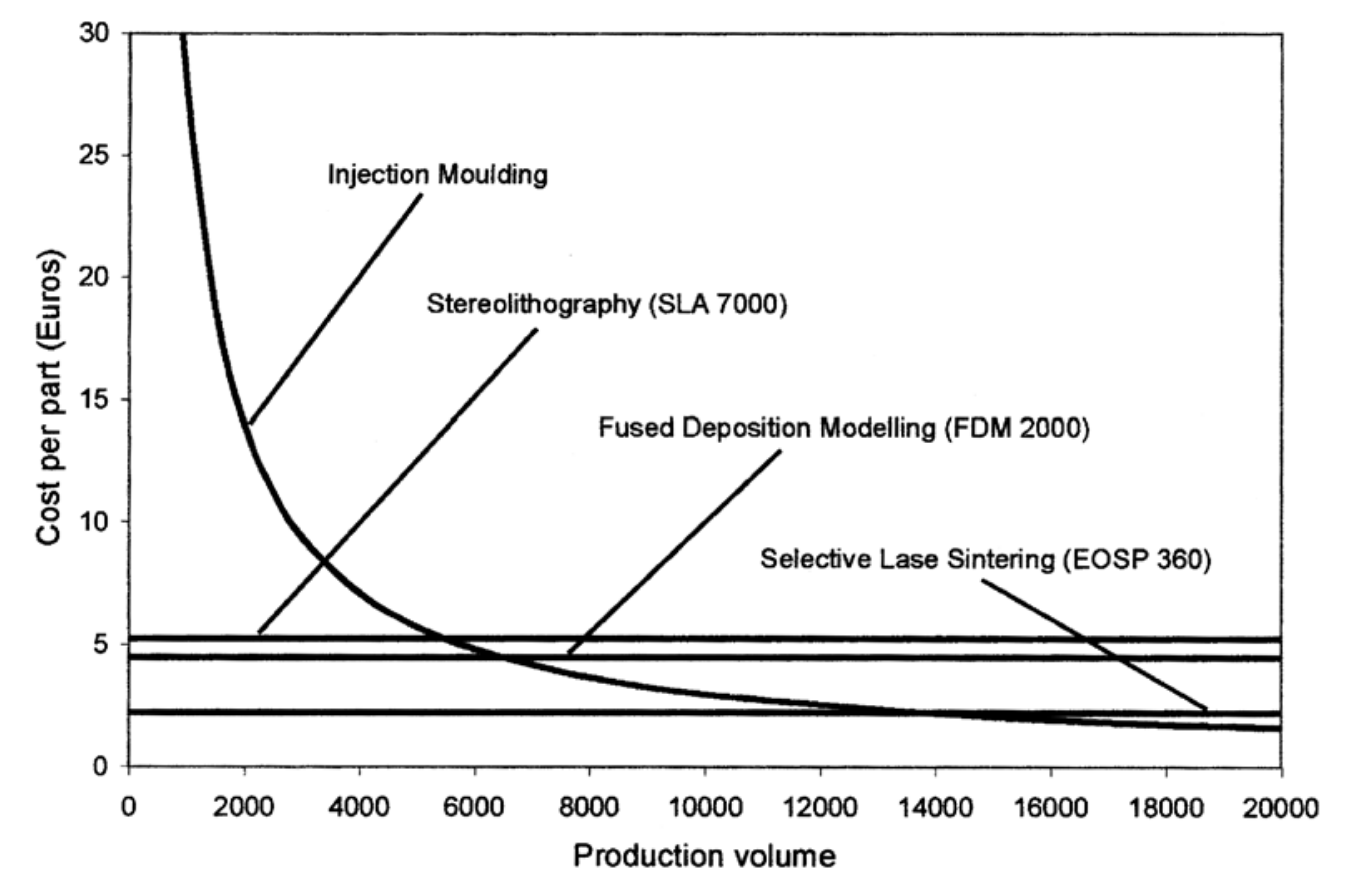
\includegraphics[width=0.55 \textwidth]{Images/costs.png}
    \caption[Traditional processes vs AM costs.]{Cost comparison for the manufacturing of a small plastic lever using different processes \cite{hopkinson_analysis_2003}.}
    \label{fig:costs}
\end{figure}
Furthermore, the initial machinery expenses were the primary cost factor in AM technologies. The authors believe these costs will decrease with mass adoption and technological advancements, thus reducing overall production costs. The real turning point for widely spread 3D printing occurred in the early 2010s, when patents for some polymers used in fused deposition modeling systems (FDM) expired. There was an absolute explosion of FDM 3D printer producers. We will discuss FDM shortly. Nowadays, additive manufacturing is employed in the production of small batches of finished products, sometimes even single-unit batches of highly customized products, or also in the prototyping phase.
These manufacturing processes do not intend to replace the traditional ones but rather allow us to expand the limits of what we can build. It is important to understand that additive manufacturing allows us to obtain components with mechanical functionalities and complexity unimaginable with traditional manufacturing processes but cannot be the only approach to production (at least for now).

%%%%%
%%%%%

% Additive Manufacturing Process Categories >>>
\section{Additive Manufacturing Process Categories} 
\label{sec:AMproc}
According to ISO/ASTM 52900 \cite{organization_isoastm_2015} and \citeauthor{gibson_additive_2015} (2015) there are seven different types of AM technologies: 
\begin{itemize}
    \item \textbf{Vat photo-polymerization processes} (VP). VP processes use radiation-curable resins or photopolymers that can be solidified using controlled light sources, usually ultraviolet radiation. Typically, it involves galvanometers to direct a laser beam or multiple directional light sources, such as controlled LEDs. The polymers used in this printing technology are usually acrylate-based or epoxy resins and industrial ceramic materials, such as alumina, zirconia, and silicon nitride. In recent years, new materials have been developed for the production of investment casting patterns \cite{3d_systems_investment_2023}, but also high technical performance material such as Cyanate Ester, which is used with Carbon Digital Light Synthesis\textsuperscript{TM} to produce pump turbines capable of withstanding high pressures (up to \numrange[range-phrase = --]{3800}{4000}\unit{\mega\pascal}) \cite{carbon_3d_carbon_2023}. The major advantages of this technology are the high level of accuracy of the finished products (up to \SI{0.05}{\milli\metre}), relatively high speed of manufacturing, and the variety of print sizes (ranging from tiny printers to larger ones, up to \qtyproduct{1000 x 800 x 500}{\milli\metre}. The disadvantages are that the finished prints require significant post-processing and that printers and the manufacturing process are still quite expensive. Moreover, material choices are limited to photopolymers only.
    \item \textbf{Fused filament fabrication} (FFF). FFF systems selectively extrude material as a filament through a heated nozzle. These processes are also called fused deposition modeling (FDM). These printers have a nozzle that is free to move in the horizontal plane and a system that moves it up and down along the z-axis (usually a threaded tube), allowing layer-wise material deposition. Typically employed materials are waxes, polyamide, acrylonitrile-butadiene-styrene, polyphenyl sulfone, polycarbonate, ceramics, and biocompatible or biodegradable materials. The main advantages of FFF systems include their widespread popularity and economic accessibility, as well as the variety of materials that can be used, such as ABS, which provides excellent structural properties, or PLA (polylactic acid), which can be extruded at relatively low temperatures and it is compostable. The drawbacks of this technology include lower print speeds and a lower achievable minimum resolution compared to other processes. We usually need to do some post-processing operations to achieve a satisfactory finishing.
    \item \textbf{Material jetting systems} (MJ). MJ is a technique that allows 3D printing of a piece using tiny droplets of liquid material selectively deposited onto a plate. Material jetting can be seen as the natural evolution of standard 2D inkjet printers but in three dimensions. MJ printers can use "cartridges" of materials and colors like traditional inkjet printers. One of the main advantages of MJ is the possibility of printing high-resolution multi-colored or multi-material objects. Initially, the materials used with this technology were waxes. Still, in recent years, the focus has been more on the deposition of acrylate photopolymers, in which droplets of materials are solidified with a UV lamp directly attached to the printing nozzle. The main advantages of MJ are the reduced material waste, as the deposition process is extremely precise (droplets of \numrange{25}{120} \unit{\micro\meter} at a rate of \numrange{0}{2000} \unit{drops / \second}), and the possibility of using different materials and colors simultaneously. The disadvantages of this solution are mostly the limited number of usable materials since only polymers and waxes or materials that are not excessively dense can be employed. Furthermore, the equipment required is relatively cheap, and the process can reach a remarkable printing speed.
    \item \textbf{Binder jetting systems}. Binder jetting is very similar to MJ. In binder jetting, a liquid binding agent called "binder" is selectively deposited in tiny droplets to solidify material powder, allowing different layers of powder to stick together. Due to the production method, the final objects may only sometimes be suitable for withstanding significant structural stresses and often require a long post-processing phase, which could increase variable costs. Binder jetting can be used with thermo-plastic polymers, metals, and ceramic materials. Compared to MJ, the significant advantages of this technology are the ability to use a much more vast range of materials and the higher printing speed. Moreover, it is possible to mix different powders to obtain final objects with specific mechanical features. However, printed parts often require a lot of post-processing work to improve the mechanical features and the finishing of the pieces.
    \item \textbf{Laminated object manufacturing} (LOM). In sheet lamination or laminated object manufacturing (LOM), layers of material are bonded together to form the final object. There are two possible approaches: "bond-then-form" and "form-then-bond." In the first case, the laminate is positioned and bonded to the substrate and then cut following the model contour. In the second case, the laminate material is cut, placed on the substrate, and bonded to the underlying layer. LOM techniques allow the usage of wood, thermo-plastic polymers, industrial ceramics, paper, polyvinyl chloride, and composite materials. The significant advantages of LOM are the ability to print large parts quickly and the lower equipment fixed costs compared to other types of AM processes.
    \item \textbf{Powder bed fusion} (PBF):  In these additive manufacturing techniques, a concentrated energy source is used to melt layers of powder selectively. Usually, the energy source is a laser (Selective Laser Sintering or SLS) or an electron beam (Electron Beam Melting or EBM), and the materials used can be polyamides, nylons, elastomers, and metals such as stainless steel, titanium, aluminum, cobalt, and copper. This AM technique is widely used for direct manufacturing and allows for producing finished objects with excellent mechanical properties and surface finishes.
    \item \textbf{Direct energy deposition} (DED): In DED, a concentrated heat energy source is used to melt material as soon as it is deposited selectively. Depending on the energy source used, we can further divide the processes into laser, electron beam, and plasma metal deposition. Moreover, depending on the shape of the material used, we can distinguish between powder-fed and wire-fed systems. Finally, depending on the direction in which the material is fed, we can distinguish between off-axis feeding, in which a side-mounted incident nozzle deposits the material, and coaxial feeding systems, in which the powder or wire material is deposited co-axially with the energy beam. The main advantage of DED is that it can be used to add parts to existing components or for repairs with a minimum need for support structures. There are several powders and printing area sizes available. However, DED has a lower accuracy compared to PBF, which makes DED unsuitable for producing complex shapes.
    \end{itemize}

% <<< End of Additive Manufacturing Process Categories

%%%%%
%%%%%

\section{Aim and Structure of the Work}
\label{sec:aimwork}
\begin{figure}
    \centering
    \subfloat[\label{fig:bugatti}]{
        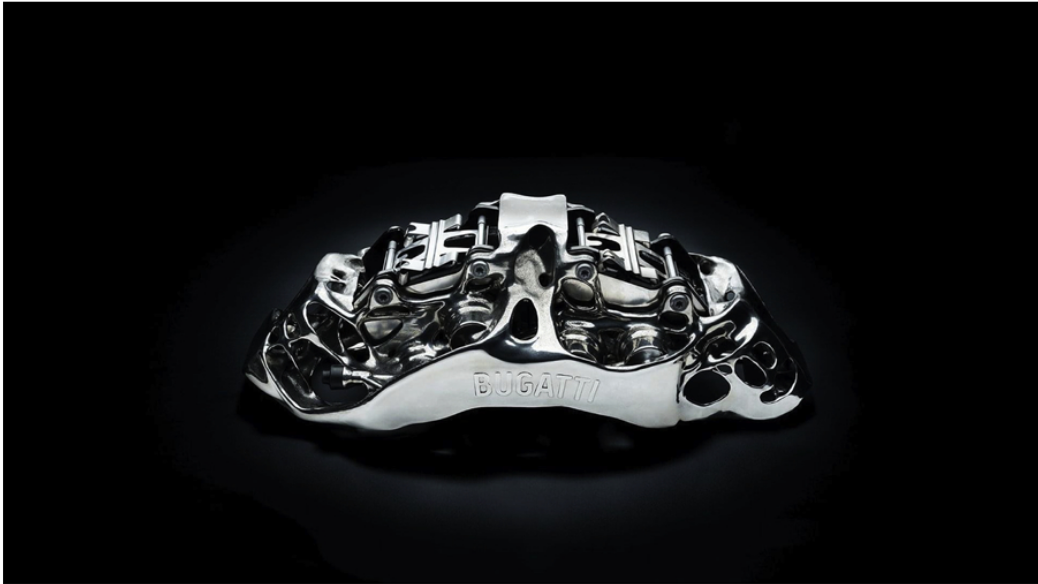
\includegraphics[scale=0.4]{Images/bugatti.png}
    }
    \quad
    \subfloat[\label{fig:supporto}]{
        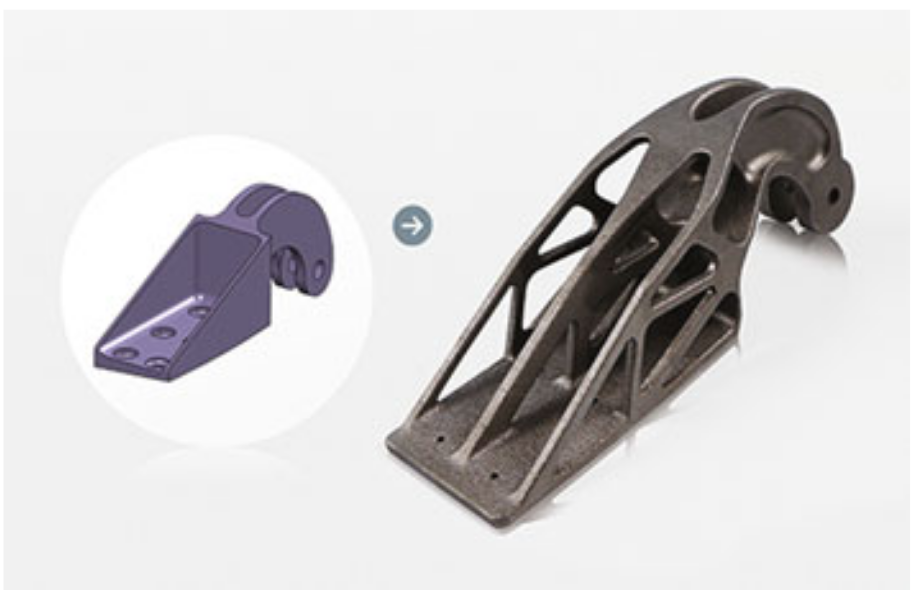
\includegraphics[scale=0.4]{Images/supporto.png}
    }
    \caption[Functional AM part printed in metal.]{On the left, a Bugatti brake caliper, one of the world’s largest functional parts produced in titanium alloy Ti6Al4V by AM. On the right, we can see support used in the aerospace industry. From \citeauthor{du_plessis_beautiful_2019}.}
    \label{fig:funcpart}
\end{figure}
In recent years, additive manufacturing processes for metallic parts, especially the so-called powder bed fusion processes, have revolutionized various industries, including aerospace, automotive, and energy. PBF processes are currently the most promising AM technology for printing structurally sound and functional components. Indeed, these processes are also used to create components that play a critical role during their use, often for safety reasons. Consider, for instance, the importance of the brake system shown in Fig. \ref{fig:bugatti}. Imagine the repercussions if the braking system failed on a Chiron that is speeding at \SI{350}{\kilo\metre /\hour}, or if aerospace support, like the one in Fig. \ref{fig:supporto}, may break, causing a \SI{8500}{\metre} fall of a heavy piece. For these reasons, as shown in Fig. \ref{fig:vchain}, the AM chain is particularly articulated, mainly due to the importance of the testing and certification phases. Data collected from process monitoring in AM presents a unique opportunity (compared to traditional manufacturing) for early defect detection or new non-destructive testing techniques.
\begin{figure}
    \centering
    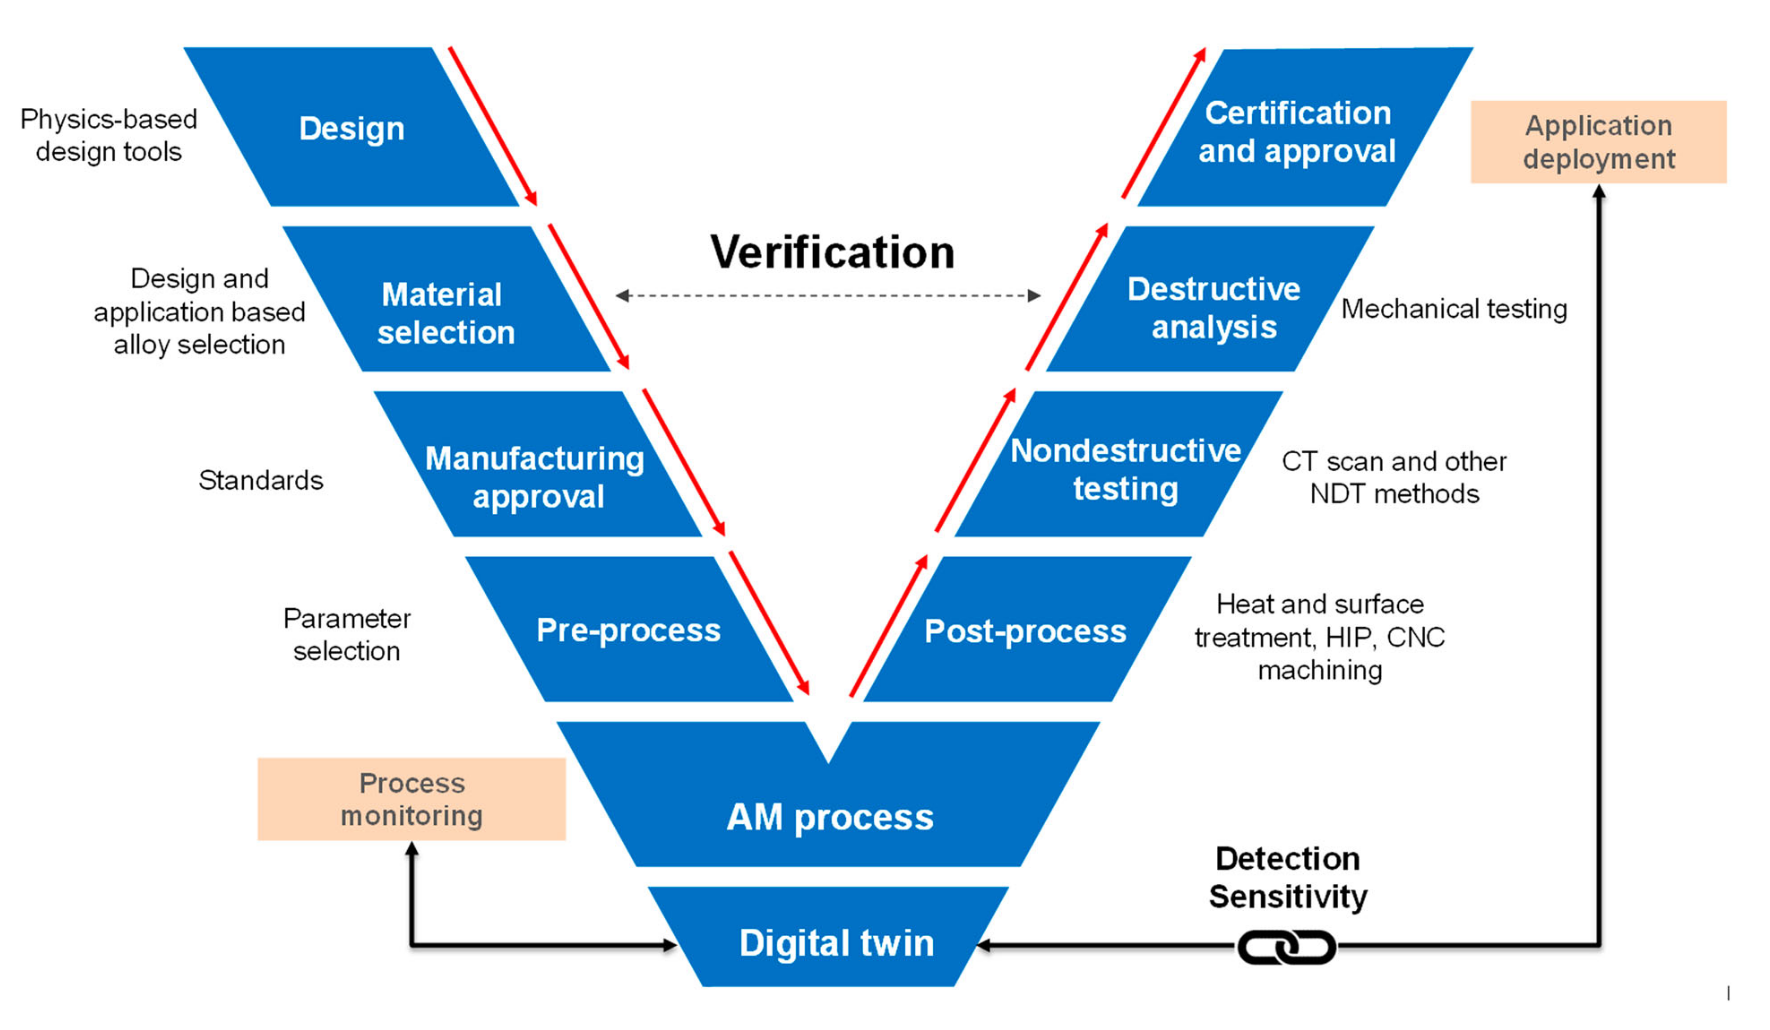
\includegraphics[width=0.65 \textwidth]{Images/v.png}
    \caption[AM process chain.]{V-shaped process chain for AM from design to certification \cite{moshiri_performance_2023}.}
    \label{fig:vchain}
\end{figure}
Quality control, defect detection, and ensuring the production process adheres to standards are crucial now more than ever. The temperature, particularly in additive manufacturing for metallic parts, significantly influences the mechanical properties of the finished product, as demonstrated in \citeauthor{williams_situ_2019} (2019). Indeed, the temperatures reach much higher peaks, and the cooling process is more dynamically complex. Anyone who has experience with "classical" FDM 3D printing for PLA would notice that the filament cools down in seconds. On the other hand, with metallic PBF printing, one must wait considerably longer before the final piece is extracted from the production chamber. Moreover, many additional factors could affect the temperature reached by the material during the PBF printing process and the consequent cooling process. This thesis aims to present a state-of-the-art review of identifying the so-called hot spots in PBF processes using machine learning algorithms. Hot spots are localized areas characterized by elevated temperatures for a sustained time and slower cooling drift, often attributable to their proximity to adjacent loose powder. The overheating leads to defects in the finished product.

This thesis is structured as follows. Chapter~\ref{ch:Metal_AM}, I will comprehensively describes PBF processes for 3D printing of metal parts, the necessary technologies, materials, and some potential applications. Chapter~\ref{ch:defects} outlines the most common defects in PBF processes, with a particular emphasis on the aforementioned hot spots, their causes, and the different monitoring systems used in AM. Chapter~\ref{ch:state_ot_the_art} is a literature review to present the state-of-the-art in hot spots detection using machine learning algorithms. The methods for the systematic review is explained in Appendix~\ref{ap:research}. Chapter~\ref{ch:baggingvoronoi} presents the bagging voronoi classification algorithm as an innovative approach that might lead to a deeper understanding of the hot spots phenomenon leveraging functional data, as well as providing a powerful non-destructive analysis tool for thermal profiles. Chapter~\ref{ch:conclusions} conclude the thesis and propose some research streams that could be explored further. Finally, Appendix~\ref{ap:Python}, proposes a simple Python \cite{python_software_foundation_python_2023} implementation of the algorithm proposed in Chapter~\ref{ch:baggingvoronoi}.
% <<< End of Introduction


% PBF Processes >>>
\chapter{Powder Bed Fusion Processes}
\label{ch:Metal_AM}%
\setlength{\tabcolsep}{10pt}
In this Section, I will provide a comprehensive overview of powder bed fusion (PBF) processes in metal additive manufacturing. In Section \ref{sec:pbf_proc}, we will discuss how 3d printers for metal PBF work, in Section \ref{sec:metalpowders} we will discuss about the powders used in those processes, while in Section \ref{sec:matterint}, we will delve into the physical process that allows the selective fusion of metal powders into the finished product. Lastly, in Section \ref{sec:examplesPBF} we will discuss some applications for metal PBF processes.

% Powder Bed Fusion Processes >>>
\section{Powder Bed Fusion Processes}\label{sec:pbf_proc}
As we have already discussed in Section \ref{sec:AMproc}, we can divide powder bed fusion processes into laser powder bed fusion, also called selective laser sintering (SLS), or electron beam powder bed fusion, also called electron beam melting (EBM). Although the two processes are based on two different technologies and some differences in printer components, they are based on the same fundamental idea: selectively melting metallic powders using external energy sources. All PBF 3D printers consist of two basic components: the powder bed, which is a container that can move along the z-axis, and a highly concentrated energy source. 

% SLS >>>
\subsection{Selective Laser Sintering}
\label{subsec:LPBF}
\begin{figure}
    \centering
    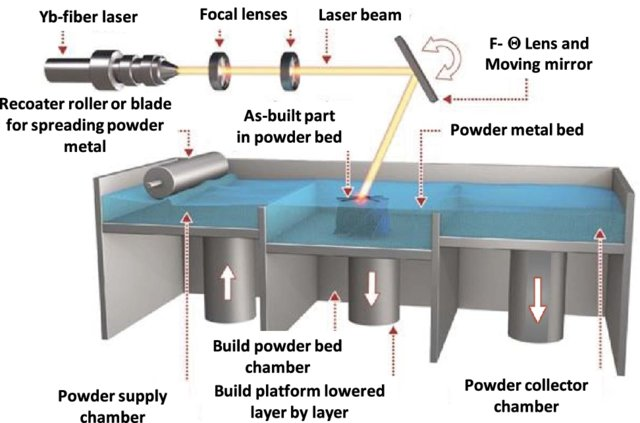
\includegraphics[scale=1.2]{Images/PBF.jpg}
    \caption[Laser PBF in AM.]{Laser powder bed fusion process in additive manufacturing. Adapted from \cite{ozel_focus_2020}.}
    \label{fig:PBF}
\end{figure}
Now, we will discuss the SLS printing process from start to finish. Firstly, the plate mounting is calibrated, and a vacuum atmosphere is created inside the printer chamber, or a regular flow of inert gas is introduced to obtain controlled and uniform melting of the metal powder to minimize oxidation and degradation of the powdered material. Directing an inert gas is preferred to maintaining a vacuum atmosphere in an industrial context mainly for two reasons. First, maintaining a vacuum atmosphere throughout the printing process requires much effort. Second, reducing the pressure in the process chamber can lower the metals' boiling point, leading to an excessive amount of smoke. The mixture of vaporized metal and smoke can affect the effectiveness of the laser. Indeed, a laser is an optical device and, as we all know, microparticles suspended in the air could deflect the laser beam. Once the inert gas flow is established, the roller or the blade responsible for distributing the powder performs a rapid powder re-coating. Then an electric resistor located under the powder bed preheats the powder at a temperature of about \SI{500}{\degreeCelsius}. This operation helps to reduce the gap between the temperature of the chamber and the metal's melting temperature and also helps maintain a uniform temperature within the build tray. This is necessary to prevent the warping of the part during the build due to non-uniform thermal expansion and contraction, which will lead to cracks and fractures (see Section \ref{sec:defects}). After these preliminary operations, the printing process can begin. A scanning system composed of a laser diode and a galvanometric mirrors system selectively melts the metal, alternating layer after layer with the powder distribution blade. LASER is an acronym that stands for "light amplification by stimulated emission of radiation," and it is a monochromatic beam of photons characterized by low divergence and a focal spot size of \numrange[range-phrase = --]{30}{80}\unit{\micro\metre}. Laser equipment can generate powers in the range of thousands of watts and can focus to beam spot sizes of fractions of a millimeter. These small spot sizes have the potential to create minuscule molten pools, reaching a velocity of up to several meters per second. Nowadays, almost all lasers used in AM rely on active optical fiber sources. A schematic representation can be seen in Fig. \ref{fig:detailedfiber}. 
\begin{figure}
    \centering
    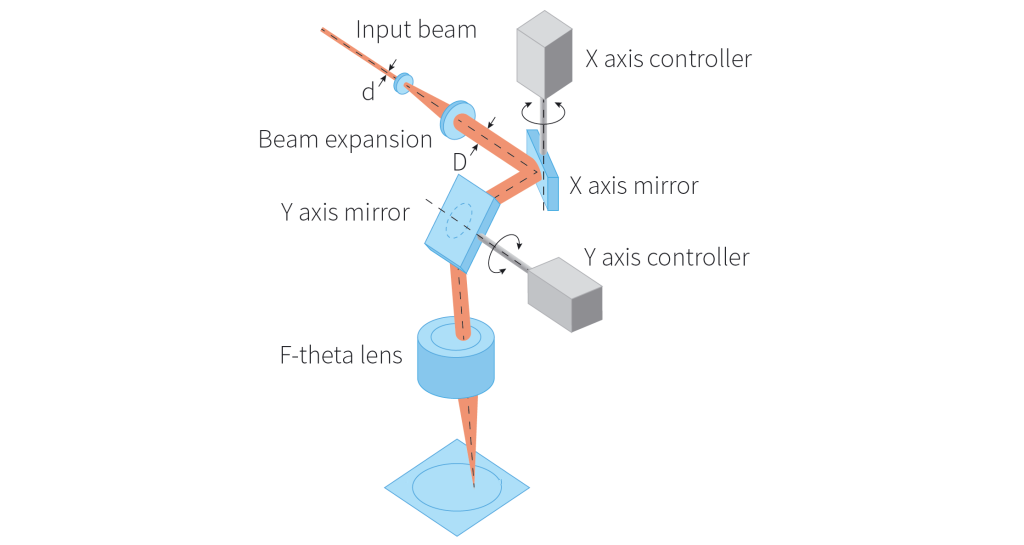
\includegraphics[scale=0.4]{Images/galvanometro.png}
    \caption[Galvanometric system.]{Dual-axis galvanometric system.}
    \label{fig:galvano}
\end{figure}
The energy transferred from the laser to the powder bed depends on the laser power (\numrange[range-phrase = --]{100}{1000}\unit{\watt}), the light-absorbing capacity of the material, and the scanning speed, which can be controlled (and it's limited) by the angular velocity of the galvanometer. The galvanometer system, Fig. \ref{fig:galvano}, consists primarily of two mirrors rotating along their axis, directing the laser beam to a desired point. The photon beam passes through a series of f-theta lenses that facilitate rapid laser movement and precise focusing of the laser spot. After completing the printing process, it is necessary to allow the object to cool down. Although supports are not always required, as the powder supports the object itself, they may need to be inserted to ensure uniform heat transmission during the printing and cooling phase. Once the object has cooled down, we can remove any excess powder. The excess powder can be recycled and reused after undergoing some preliminary processing and conformity controls \cite{strondl_characterization_2015}. Finally, post-processing operations can be carried out if required, such as removing any supports, surface finishing, and annealing. The latter is needed if the cooling phase inside the chamber has created an undesired microstructure in the printed piece.
% <<<SLS

%%%%%
%%%%%

% EBM >>>
\subsection{Electron Beam Melting}
\label{subsec:ebm}
In EBM printers, the process is fundamentally the same as in laser printers, with metal powder selectively fused in a powder bed, with a recoater blade to provide additional metal powder layer after layer. However, the energy source is not a laser (i.e., a beam of photons) but rather a beam of electrons. Secondly, the preheating stage is not accomplished through an electric resistor but through the electron beam. The preheating operation is one of the most significant differences between EBM and SLS. An electric current is passed through a metallic filament to produce an \emph{electron beam}, typically tungsten or tantalum. The resulting electron beam is then directed through a Wehnelt cylinder. By negatively or positively charging the cylinder, we can block or allow the passage of electrons respectively.
\begin{figure}
    \centering
    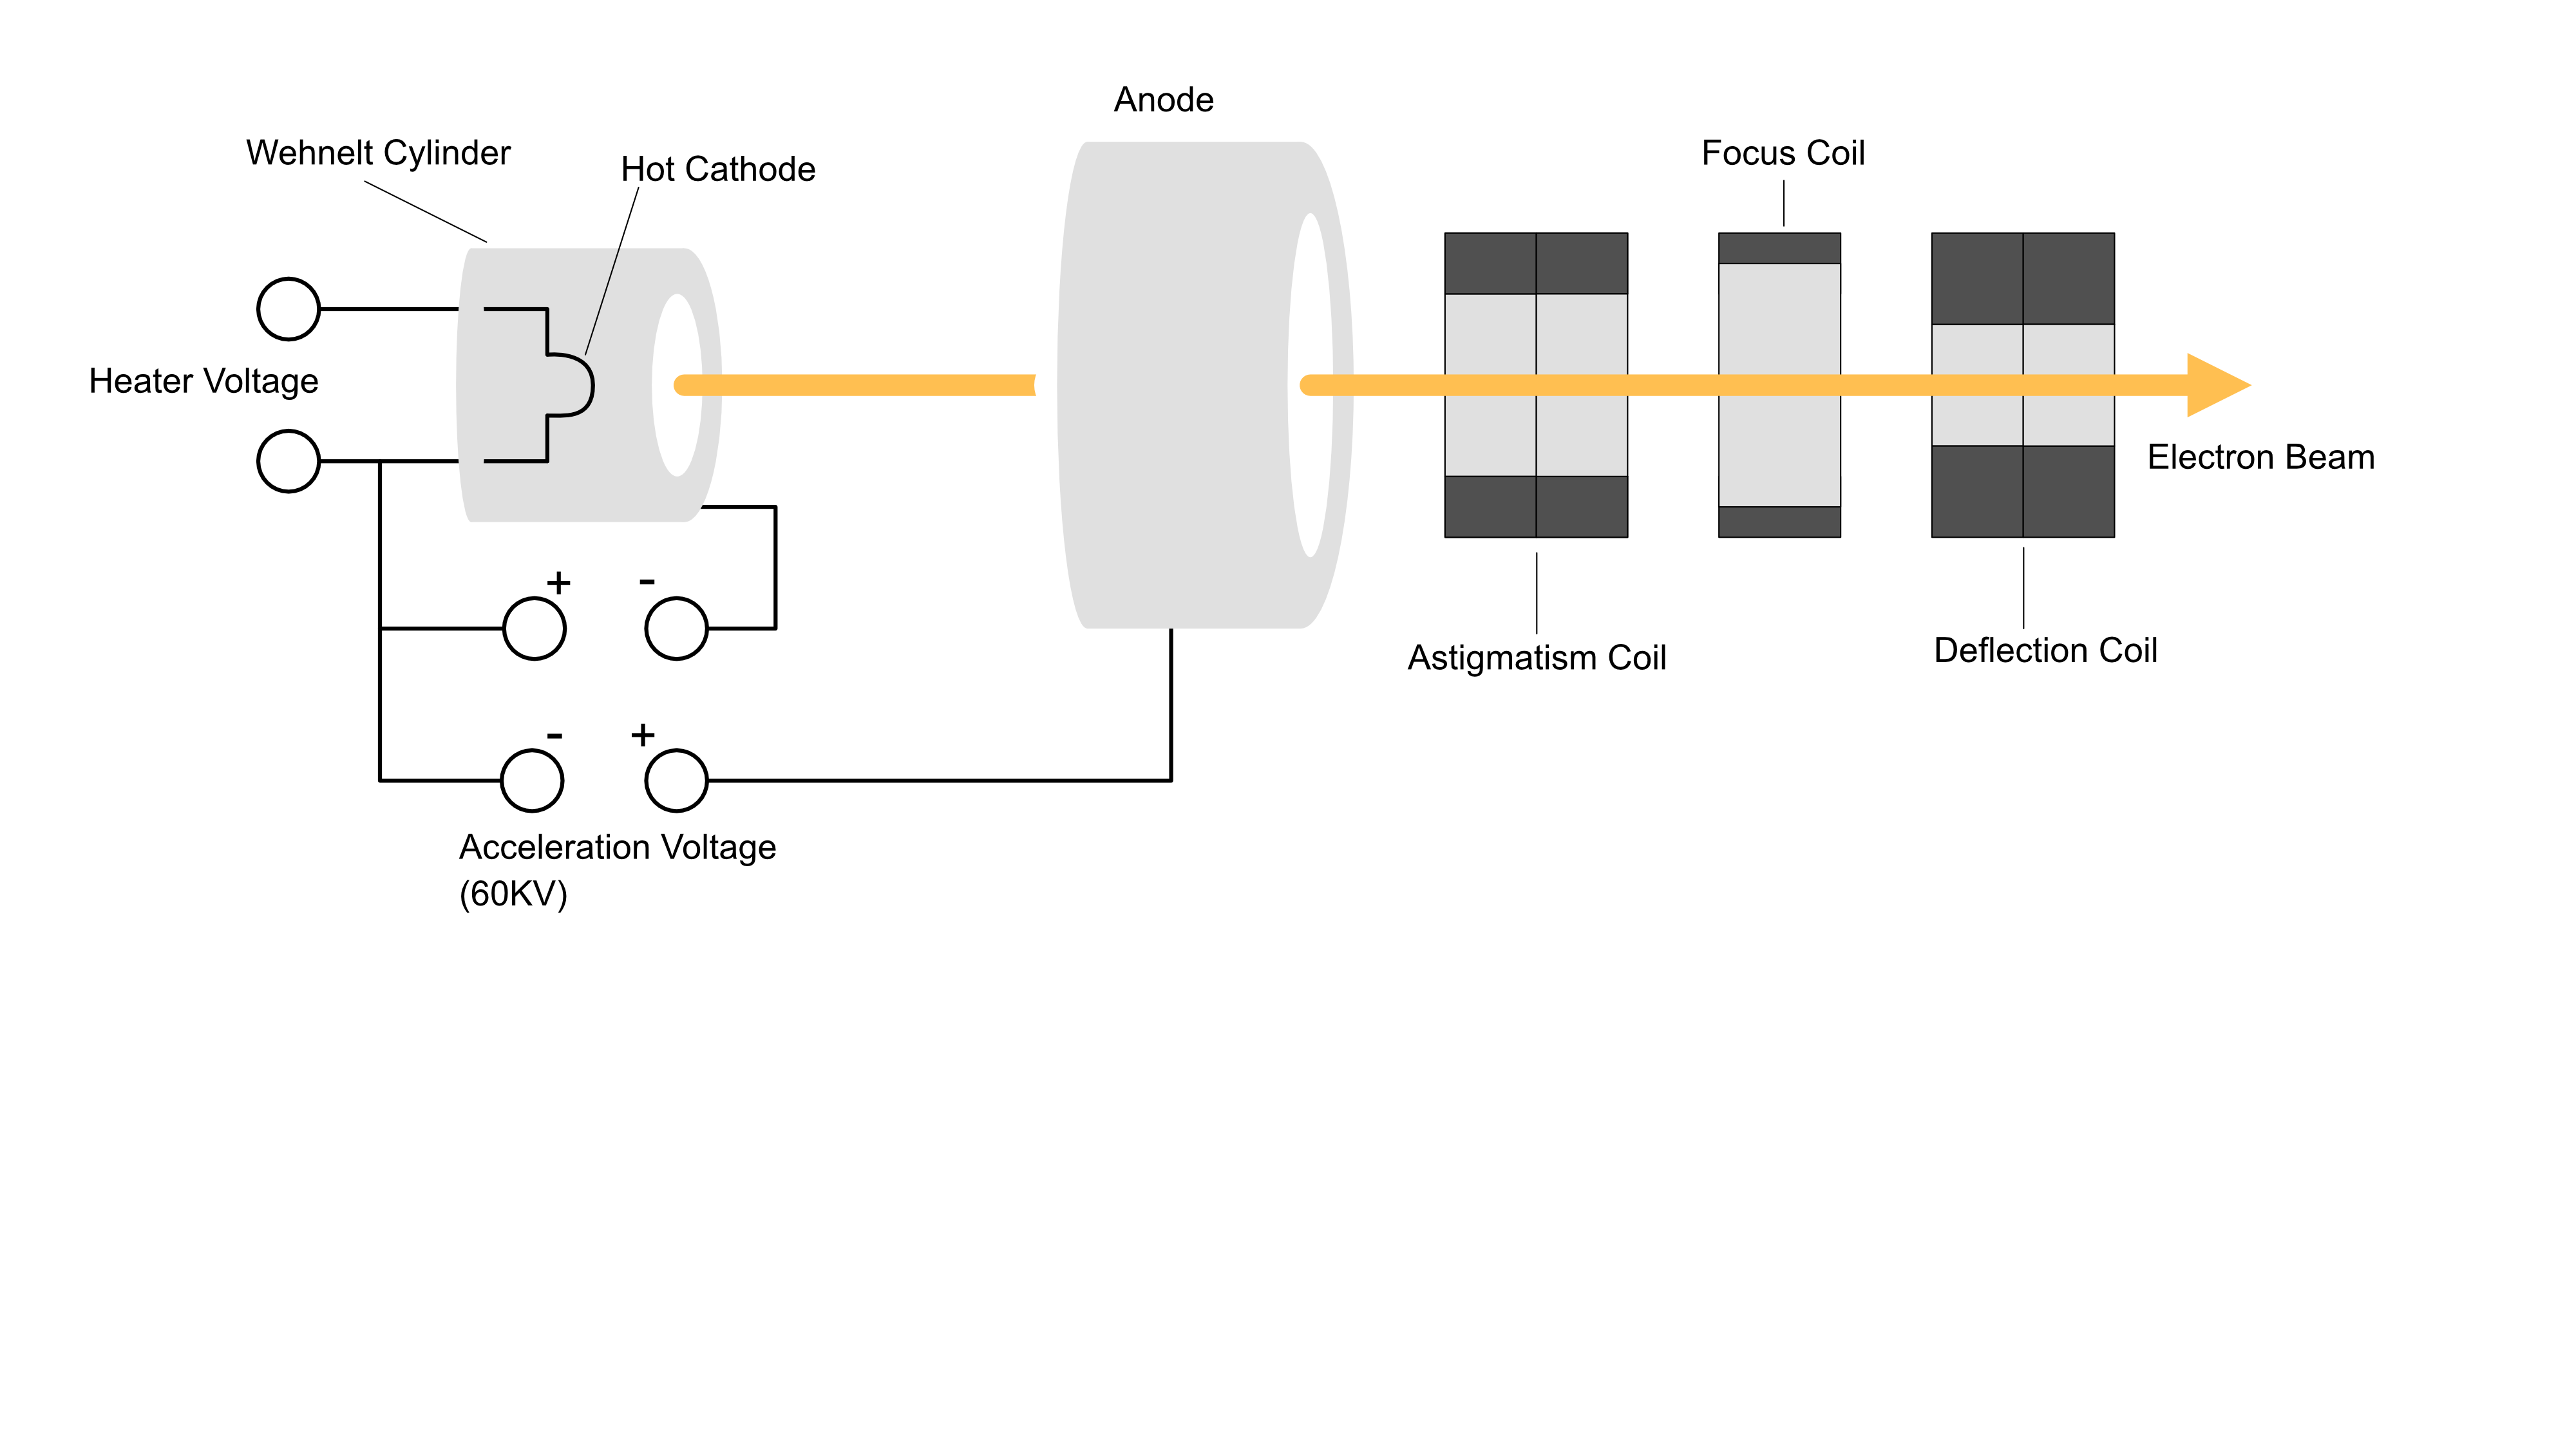
\includegraphics[width=0.75\textwidth]{Images/EBM.png}
    \caption[Electron gun schema.]{Electron gun schema.}
    \label{fig:electrongun}
\end{figure}
A diagram of the electron gun beam's structure can be seen in Fig. \ref{fig:electrongun}. Finally, the electron beam passes through an anode charged with a voltage of up to \SI{60}{\kilo\volt}, which accelerates the electrons and allows the beam to be directed into the column through magnetic lenses. Unlike SLS printers which rely on optical lenses, the lenses in EBM printers are magnetic lenses. A more comprehensive description of how magnetic lenses function will be provided in Section \ref{sssec:magneticlens}. EBM printers require a vacuum atmosphere inside the printing chamber to work correctly, and a minute amount of helium must be continuously injected into the chamber to prevent the accumulation of electric charges due to any residual electrons on the powder bed. The phenomenon will be discussed in Section \ref{subsec:ebminter}. To put the "minuscule amount" of helium required into perspective, consider that the pressure in the vacuum atmosphere inside the chamber is \SI{0.05}{\pascal}, and the pressure with helium flow is about \SI{0,2}{\pascal} (recall atmospheric pressure is \SI{1,01325e5}{\pascal}). The second significant difference, as mentioned earlier, is that the preheating phase does not occur through an electric resistor but rather through an initial scan of the electron beam that happens at two distinct moments. During the first phase, the entire powder bed is scanned, and during the second phase, only sub-regions of the powder bed that will be printed are scanned. Preheating phases help avoid the so-called "smoke effect" caused mainly by the electrostatic repulsion in the powder. Furthermore, the preheating stage is necessary for obtaining final objects with better performance and reduces the need for support structures during printing. This allows for the use of the entire volume of the powder bed container when printing and even printing multiple objects, one on top of the other, since there would be no printing supports interfering with them. This dual preheating phase causes the excess powder to solidify around printed pieces. Another structural difference of an EBM printer can bee seen in Fig. ~\ref{fig:ebm_printer}. Due to the vacuum inside the print chamber and the consequent lowering of the metal's vaporization temperature, a heat shield is required around the chamber to prevent the vaporized metal from condensing and creating a film on the entire printer structure. The heat shield acts as a physical barrier, allowing easy removal and disposal of the metal film produced during printing.
\begin{figure}
    \centering
    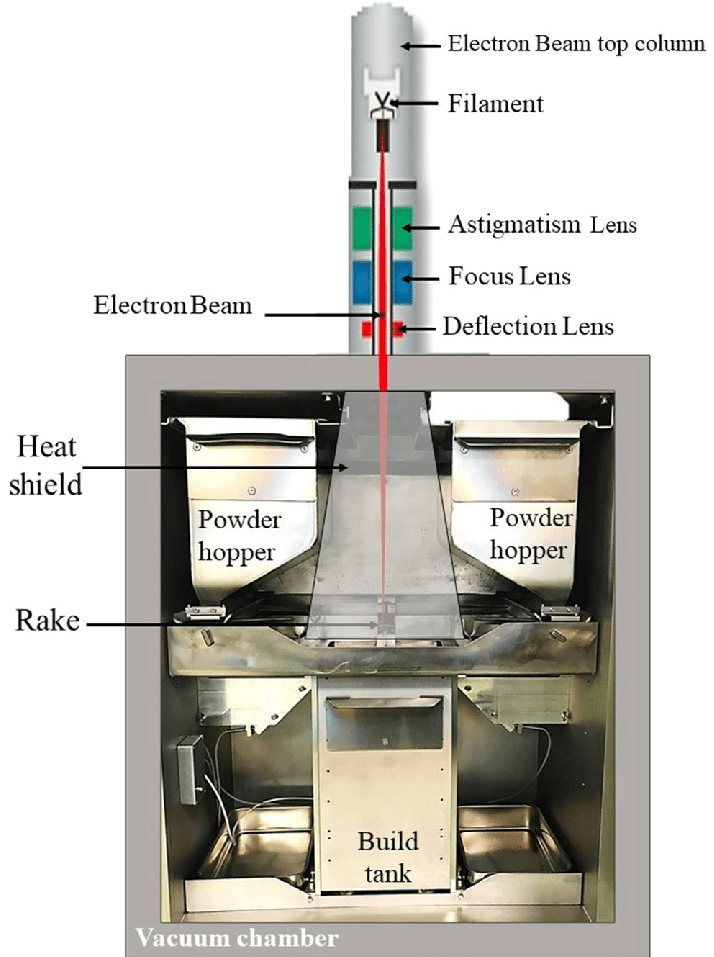
\includegraphics[scale=0.3]{Images/A-schematic-of-electron-beam-melting-EBM.png}
    \caption[EBM 3d-printer.]{Electron beam melting 3d-printer \cite{azam_-depth_2018}.}
    \label{fig:ebm_printer}
\end{figure}
\begin{table}
\small
    \centering 
    \begin{tabular}{|l l l|}
    \hline
    \rowcolor{bluepoli!40} % comment this line to remove the color
     & \textbf{EBM} & \textbf{SLS} \T\B \\
    \hline \hline
    \textbf{Energy source} & Electron beam & Laser  \T\B \\ 
    \textbf{Chamber atmosphere} & Vacuum(Almost) & Inert gas  \T\B\\
    \textbf{Scanning} & Magnetic lenses & Galvanometers \T\B \\
    \textbf{Energy absorption} & Conductivity-limited & Absorptivity-limited \T\B\\
    \textbf{Scan speeds} & Very fast & Limited by galvanometer inertia \T\B\\
    \textbf{Energy costs} & Moderate & High \T\B\\
    \textbf{Feature resolution} & \numrange{100}{200}\unit{\micro\metre} & \numrange{75}{100}\unit{\micro\metre}  \T\B\\
    \textbf{Materials} & Conductors & Polymers, metals and ceramic \T\B\\
    \textbf{Layer Thickness} & \SI{50}{\micro\metre} & \SIrange{10}{50}{\micro\metre}  \T\B\\
    \textbf{Min Wall Thickness} & \SI{0.6}{\milli\metre} & \SI{0.2}{\milli\metre} \T\B\\
    \textbf{Accuracy} & $\pm$\SI{0.4}{\milli\metre} & $\pm$\SI{0.3}{\milli\metre} \T\B\\
    \textbf{Build rate} & \numrange[range-phrase=--]{55}{80}\unit{\centi\metre^3 / \hour} & \numrange[range-phrase=--]{60}{100}\unit{\centi\metre^3 / \hour} \T\B\\
    \textbf{Powder Particle Size} & \numrange[range-phrase = --]{40}{105}\unit{\micro\meter} & \numrange[range-phrase = --]{15}{45}\unit{\micro\meter} \T\B\\
    \hline
    \end{tabular}
    \\[10pt]
    \caption{Comparison between SLS and EBM processes. Adapted from \cite{gallina_electron_2017}.}
    \label{table:slsvsebm}
\end{table}
There are also differences in the materials used for printing. In EBM printing, usually metal powder size is slightly larger than the powder used in laser printing, with a particle size of approximately \numrange[range-phrase = --]{40}{105}\unit{\micro\meter} against the \numrange[range-phrase = --]{15}{45}\unit{\micro\meter} in SLS processes. Furthermore, the metal powder must exhibit good electrical conductivity. Indeed, in EBM highly reflective metals can be used too because, unlike photons, electrons are not repelled by mirrored surfaces since they penetrate the matter thanks to the material's electrical conductivity.

To sum up what has been discussed so far, Table ~\ref{table:slsvsebm} highlights the main differences between the two processes described in previous sections.
% <<< End of EBM
% <<< End of Powder Bed Fusion Processes

%%%%%
%%%%%

% Metal Powders >>>
\section{Metal Powders for AM} 
\label{sec:metalpowders}
As we have seen in the section \ref{sec:pbf_proc}, PBF processes require metal powders. Various metallic materials can be transformed into powders suitable for additive manufacturing processes and applied in different sectors according to their mechanical properties. Table \ref{table:materialAMmetal} shows some examples of metallic materials currently available on the market and the respective industrial sectors in which they are used. In most cases, these powders are produced using atomization processes that exploit various physical methods to generate micro-particles, characterized by a more or less spherical shape and of which chemical purity depends on the method used. The inefficiency and cost of atomization processes used for manufacturing metal powders is why, in the case of specific high-quality powders, the powder price can be up to 10 times the cost of raw metal. \citeauthor{deng_origin_2020} (2020) have demonstrated that powders made of irregular micro-particles and with low chemical purity can lead to structural defects in the final parts, resulting in lower performance. Therefore, over the years, increasingly complex and expensive processes have been developed to obtain higher-quality powders.
\begin{table}[H]
\centering 
\small
    \begin{tabular}{|l l l|}
    \hline
    \rowcolor{bluepoli!40}
    \textbf{Material} & \textbf{Examples} & \textbf{Applications}\\
    \hline \hline
    \textbf{Stainless steel} & 316L, 174-PH, MS1, M300 & Food, biomedical, consumer \T\B\\
    \textbf{Ni-alloys} & In625, In718, In939 & Energy, motorsport\T\B\\
    \textbf{Al-alloys} & AlSi12, AlSi10Mg & Lightweight, aerospace, aviation\T\B\\
    \textbf{CoCr-alloys} & CoCrMo & Dental, biomedical\T\B\\
    \textbf{Ti-alloys} & Ti6Al4V, CP Ti & Biomedical, lightweight, aerospace\T\B\\
    \textbf{Tool steel} & Maraging 18Ni300 & Tooling, aerospace, automotive\T\B\\
    \textbf{Cu-alloys} & Bronze & Energy, heat exchanger\T\B\\
    \textbf{Precious} & Au, Pt, Ag & Jewellery, design\T\B\\
    \hline
    \end{tabular}
    \\[10pt]
    \caption{Material availability for metal AM.}
    \label{table:materialAMmetal}
\end{table}
\begin{figure}
    \centering
    \subfloat[\label{fig:wateratom}]{
        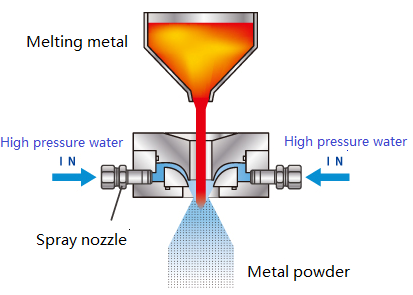
\includegraphics[scale=0.45]{Images/wateratom.png}
    }
    \qquad
    \subfloat[\label{fig:gasatom}]{
        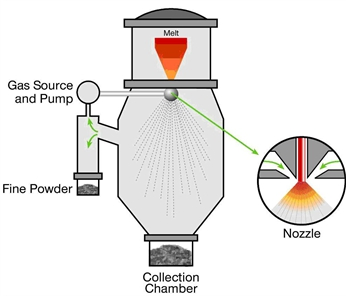
\includegraphics[scale=0.45]{Images/gasatom.png}
    }
    \\
     \subfloat[\label{fig:plasmaatom}]{
        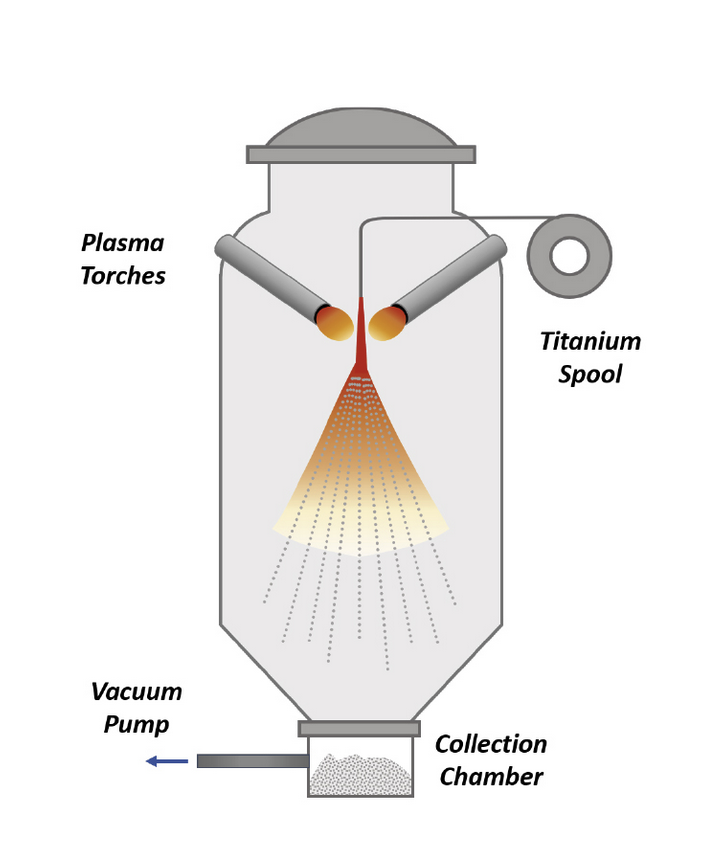
\includegraphics[scale=0.28]{Images/plasma.png}
    }
    \qquad
    \subfloat[\label{fig:repatom}]{
        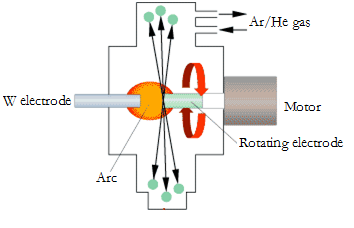
\includegraphics[scale=0.53]{Images/repatom.png}
    }
    \caption[Atomization processes.]{Water atomization process (a), gas atomization process (b), plasma atomization process (c), rotating electrode process (d) \cite{material_technology_innovations_co_rotating_2020, material_technology_innovations_co_water_2020, material_technology_innovations_co_gas_2020, inovar_communications_ltd_metal_2020}.}
    \label{fig:atom}
\end{figure}
\paragraph{Water atomization.}The process of water atomization of metals, Fig. \ref{fig:wateratom}, involves the production of small droplets of molten metal by exposing a stream of molten metal to a high-pressure jet of water. The water atomization process is typically carried out in a chamber where the molten metal is injected into a nozzle that directs the stream of liquid metal toward a high-pressure jet of water. As the molten metal comes into contact with the water, it rapidly cools and solidifies, forming tiny droplets collected at the bottom of the chamber. The size and shape of the metal droplets produced during the water atomization process can be controlled by adjusting the temperature of the molten metal, the pressure of the water jet, and the distance between the nozzle and the water jet. By handling these parameters, it is possible to produce metal powders with a range of particle sizes between \numrange[range-phrase = --]{1}{500} \unit{\micro\metre}. The output-to-input ratio for this process is approximately 95\%, which means that from \SI{1}{\kilo\gram} of raw metal, it is possible to obtain up to \SI{950}{\gram} of powder on average. Compared to other powder production methods, the water atomization process offers several advantages, including high production rates, the wide range of particle sizes obtainable, and the fact that metal ingots can be used as process input, shortening this production process's manufacturing chain. On the other hand, the process is characterized by a low chemical purity, irregular shape as can be seen in Fig. \ref{fig:waterpow}, and needs extensive post-processing operations to obtain a decent-quality product. Moreover, it cannot be used with reactive materials such as titanium and aluminum.
\paragraph{Gas atomization.} The process of gas atomization, Fig. \ref{fig:gasatom}, can be performed using a variety of gases, depending on processed metals. The most commonly used gases are inert gases such as nitrogen, argon, and helium, even if the latter is barely used in industrial applications due to its high cost. Inert gases are preferred because they do not react with the molten metal and do not introduce impurities into the metal powders. Metal ingots are molten, and the flow is rapidly solidified by exposing it to a high-pressure gas stream. This process's main advantages are its high production rate, wide range of obtainable particles, applicability to reactive materials, and ability to ensure good chemical purity. The main drawbacks are mostly related to the porosity of the resulting powder and the formation of small satellite particles.

\paragraph{Plasma atomization.} The process of plasma atomization, Fig. \ref{fig:wateratom}, involves the usage of high-temperature plasma torches to melt metal wire. We can generate a high-energy plasma by using an electric current through a non-consumable tungsten electrode and an inert gas jet to direct the welding arc into a focused area. As the molten metal droplets are expelled from the plasma jet, they rapidly solidify, sometimes also thanks to the water-cooled chamber, and break up into small, spherical powders, which are then collected in a container. The plasma atomization process offers several advantages over other powder production methods, including the ability to produce extremely spherical-shaped particles. Moreover, it can be used with reactive material. Plasma atomization can also produce powders with very high purity levels, as the high temperature of the plasma jet helps to eliminate impurities in the molten metal. However, it is more expensive than other powder production methods due to the need for specialized equipment and the high energy consumption required to generate the plasma arc. The process can also be challenging to control, as parameter variations can affect the resulting powders' size, shape, and purity. Powders produced using this method has a low size range of about \numrange[range-phrase = --]{1}{200}\unit{\micro\metre}.
\paragraph{Rotating electrode process.} In rotating electrode process, Fig. \ref{fig:repatom}, a consumable metal electrode is rotated at high speeds while an electric arc melts it in a chamber with a continuous inert gas flow. As the molten metal is exposed to the high-velocity inert gas stream, it rapidly solidifies and breaks into small droplets collected at the bottom of the atomization chamber. Due to its high cost, this production method is typically used when obtaining a metal powder with a perfectly spherical shape and without any impurities (gold, for example). If we take a look at Fig. \ref{fig:reppow}, we can easily grasp the potential of this technology in obtaining perfect spherical micro-particles.
\begin{figure}
    \centering
    \subfloat[\label{fig:waterpow}]{
        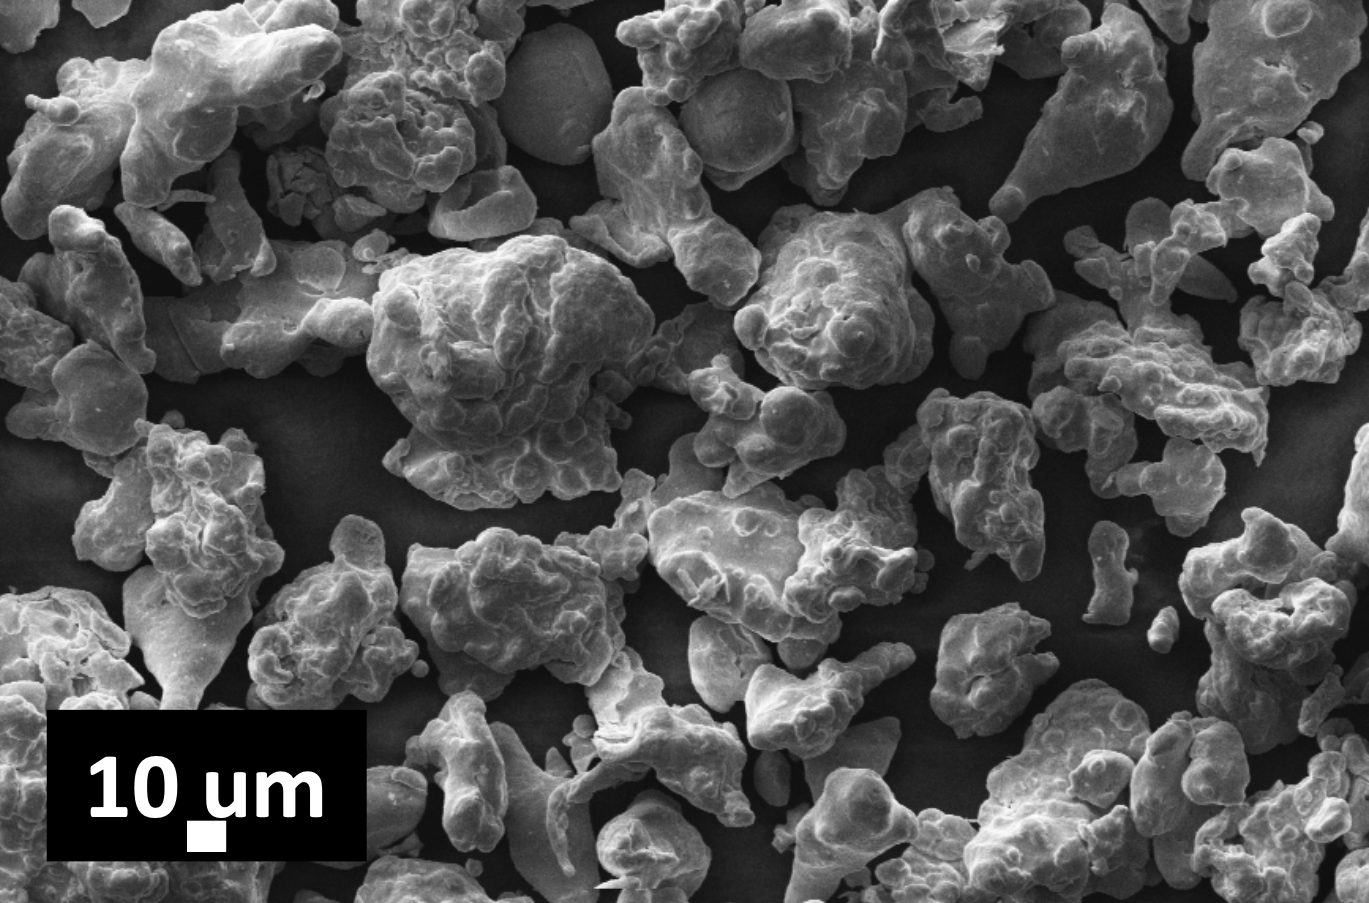
\includegraphics[scale=0.22]{Images/waterpow.png}
    }
    \qquad
    \subfloat[\label{fig:gaspow}]{
        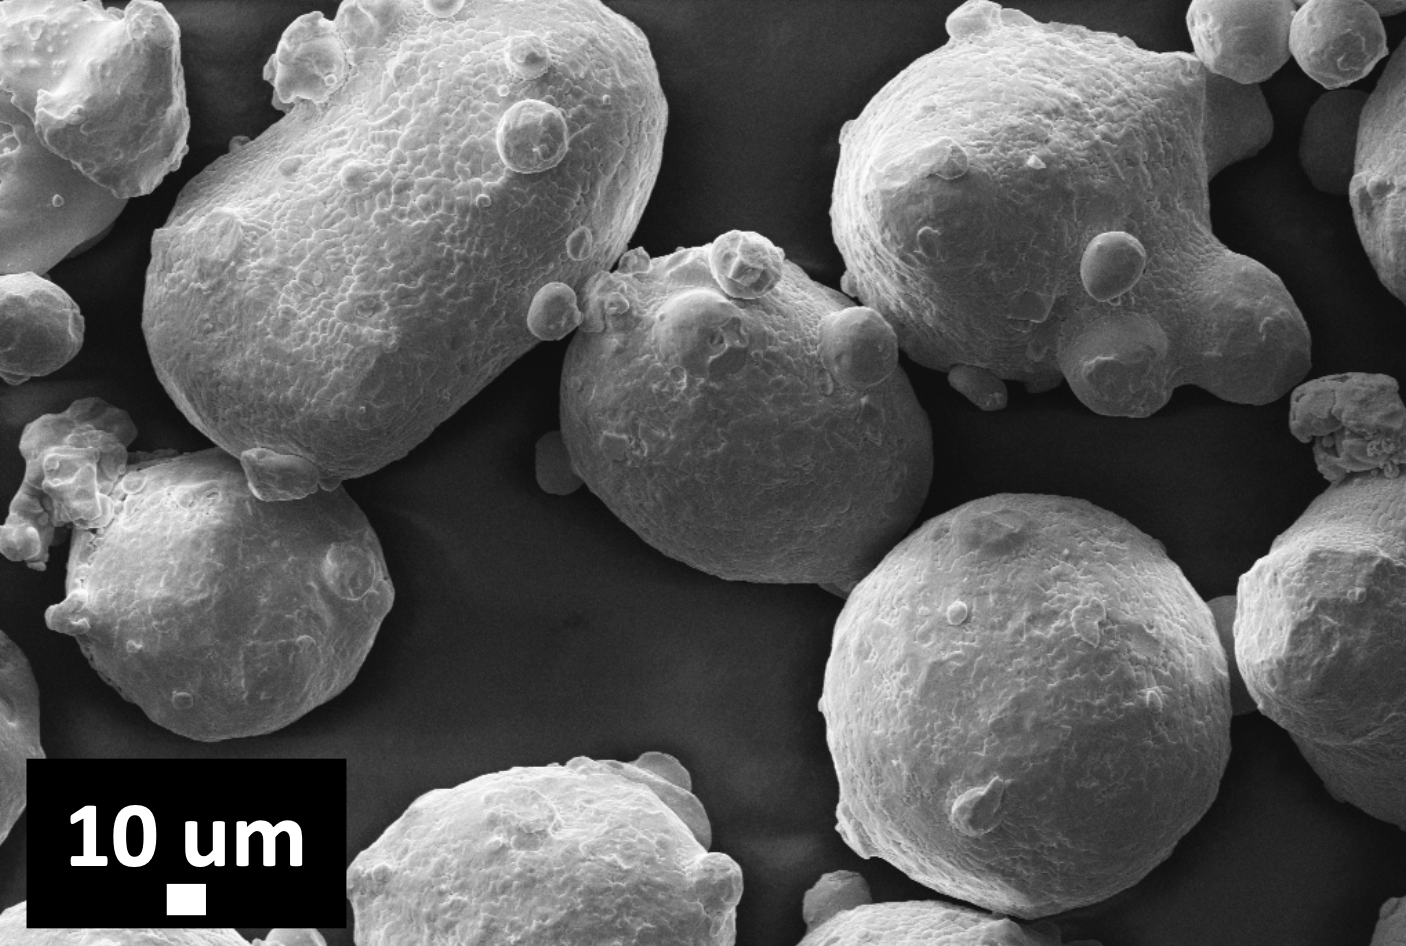
\includegraphics[scale=0.21]{Images/gaspowd.png}
    }
    \qquad
     \subfloat[\label{fig:plasmapow}]{
        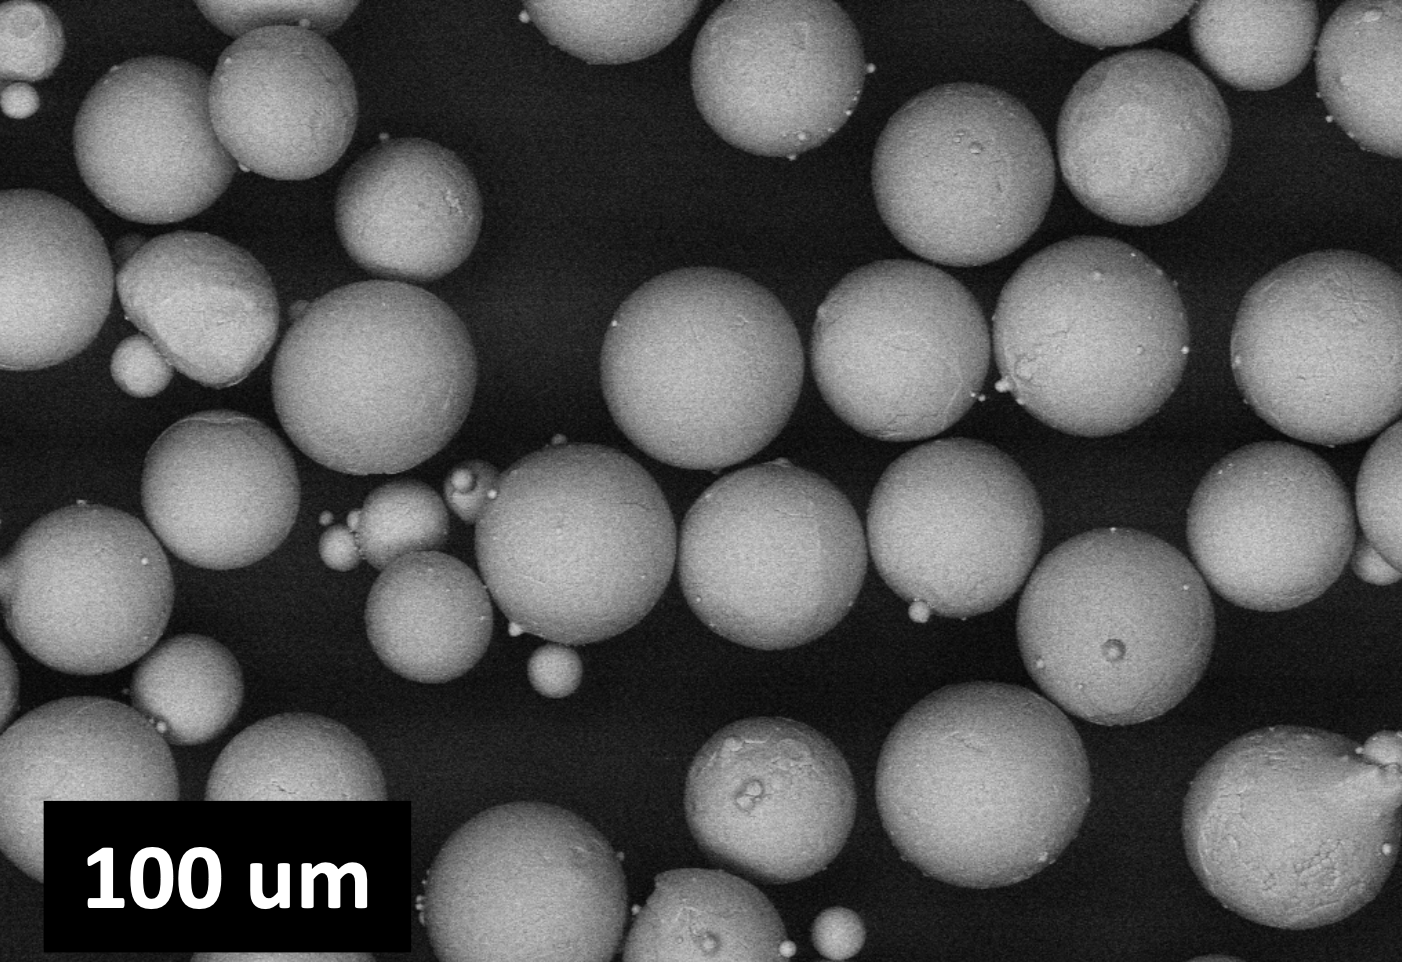
\includegraphics[scale=0.22]{Images/plasmapowder.png}
    }
    \qquad
    \subfloat[\label{fig:reppow}]{
        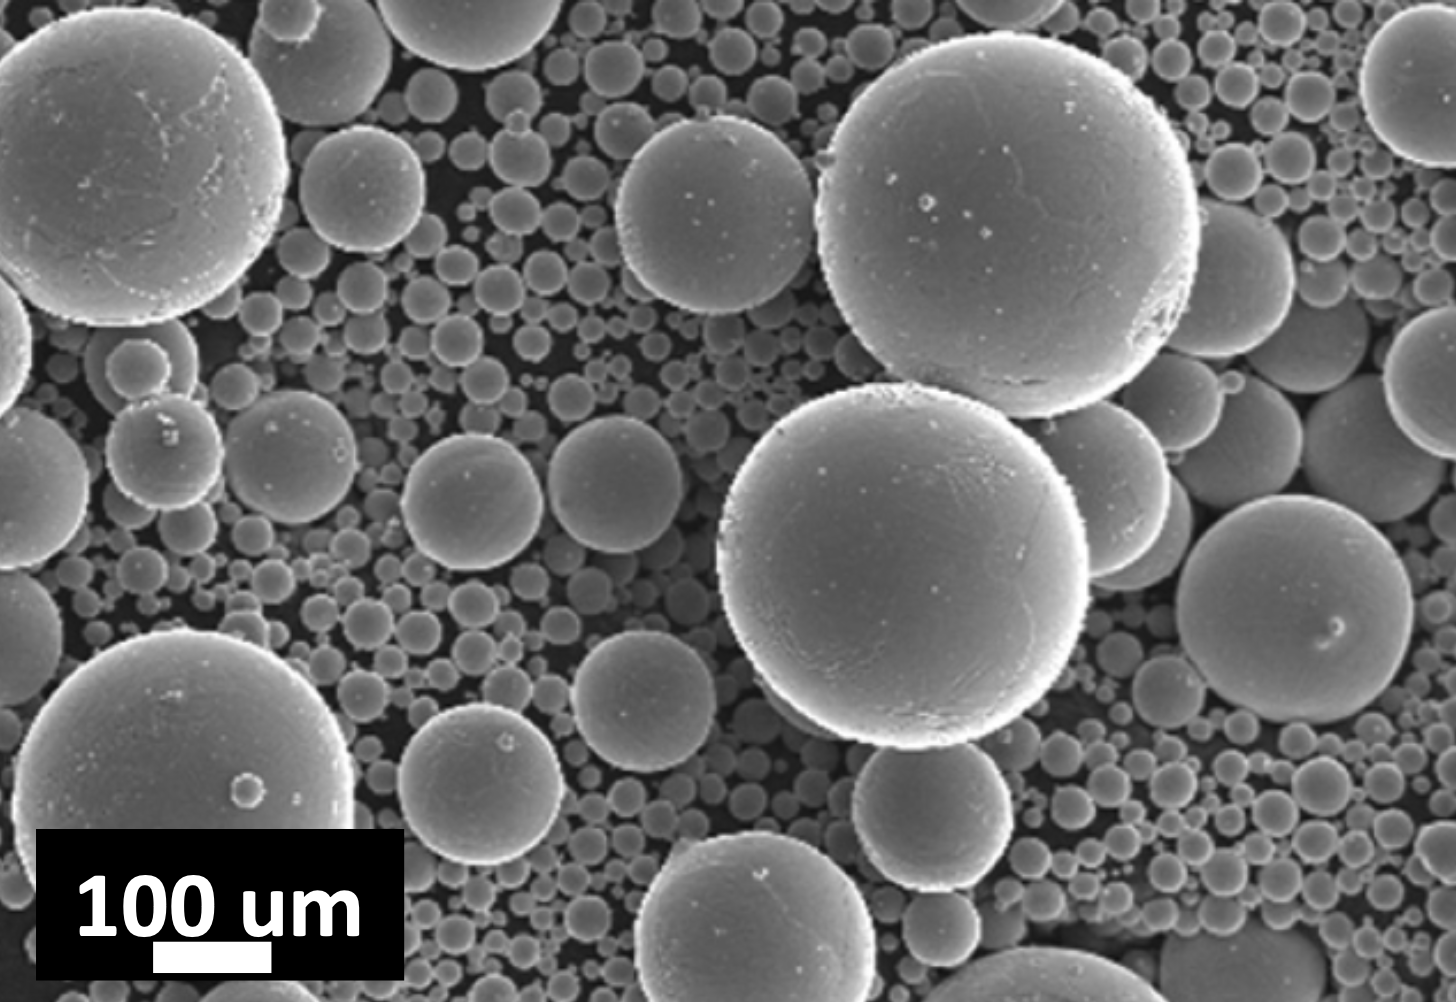
\includegraphics[scale=0.21]{Images/erppowder.png}
    }
    
    \caption[Powders from atomization processes]{Micro-particles obtained by water atomization (a), gas atomization (b), plasma atomization (c) and rotating electode process (d) \cite{slotwinski_characterization_2014}.}
    \label{fig:powders}
\end{figure}
% <<< End of Materials

%%%%%
%%%%%

% Energy matter interactions >>>
\section{Energy - Matter Interactions}
\label{sec:matterint}
This section should be regarded as "optional", and it's up to the reader's discretion whether to engage with it or not. In this section, we will delve deeply into the physical processes underlying the technologies discussed in Section \ref{sec:pbf_proc}. As said, in SLS, there is an interaction between a photon and metal powder, while in EBM, there is an interaction between electrons and metal powder. I will discuss first laser-metal interactions and then electrons-matter interaction.
\subsection{Laser - Matter Interaction}
\label{subsec:sintering}
The type and color of the laser are two essential features of SLS. Indeed, the energy transmitted to the material depends on the energy absorption characteristics of the material itself that vary according to the wavelength of the laser source. For the fusion process to be successful, metallic powder bed particles must receive enough energy to melt on the atomic level.
\begin{figure}
    \centering
    \subfloat[\label{fig:laserintera}]{
        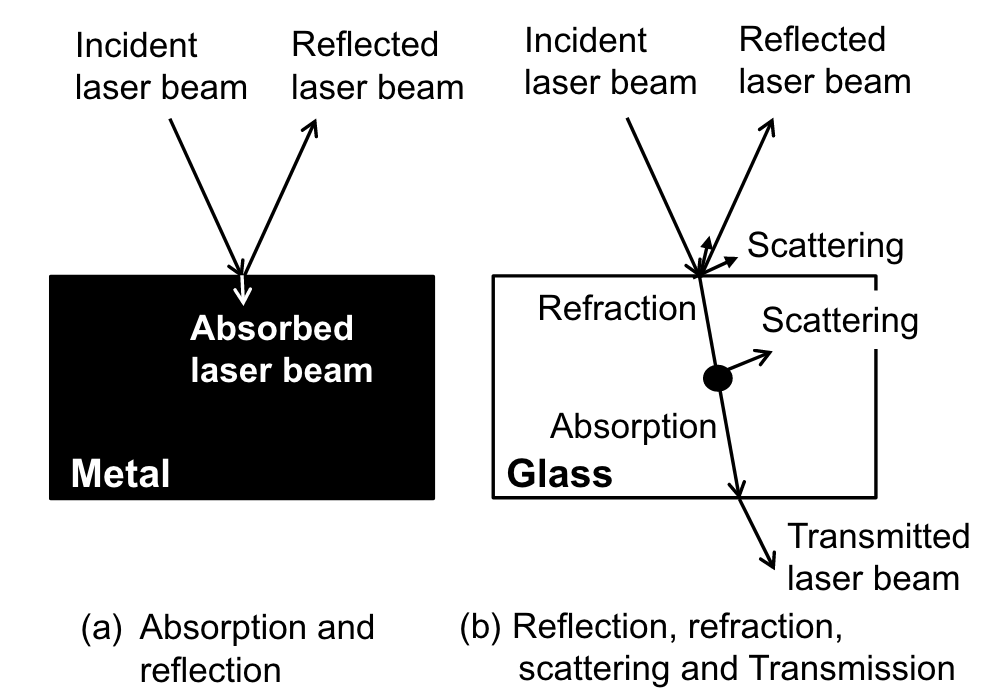
\includegraphics[scale=0.33]{Images/laser interactions.png}
    }
    \qquad
    \subfloat[\label{fig:laserintensity}]{
        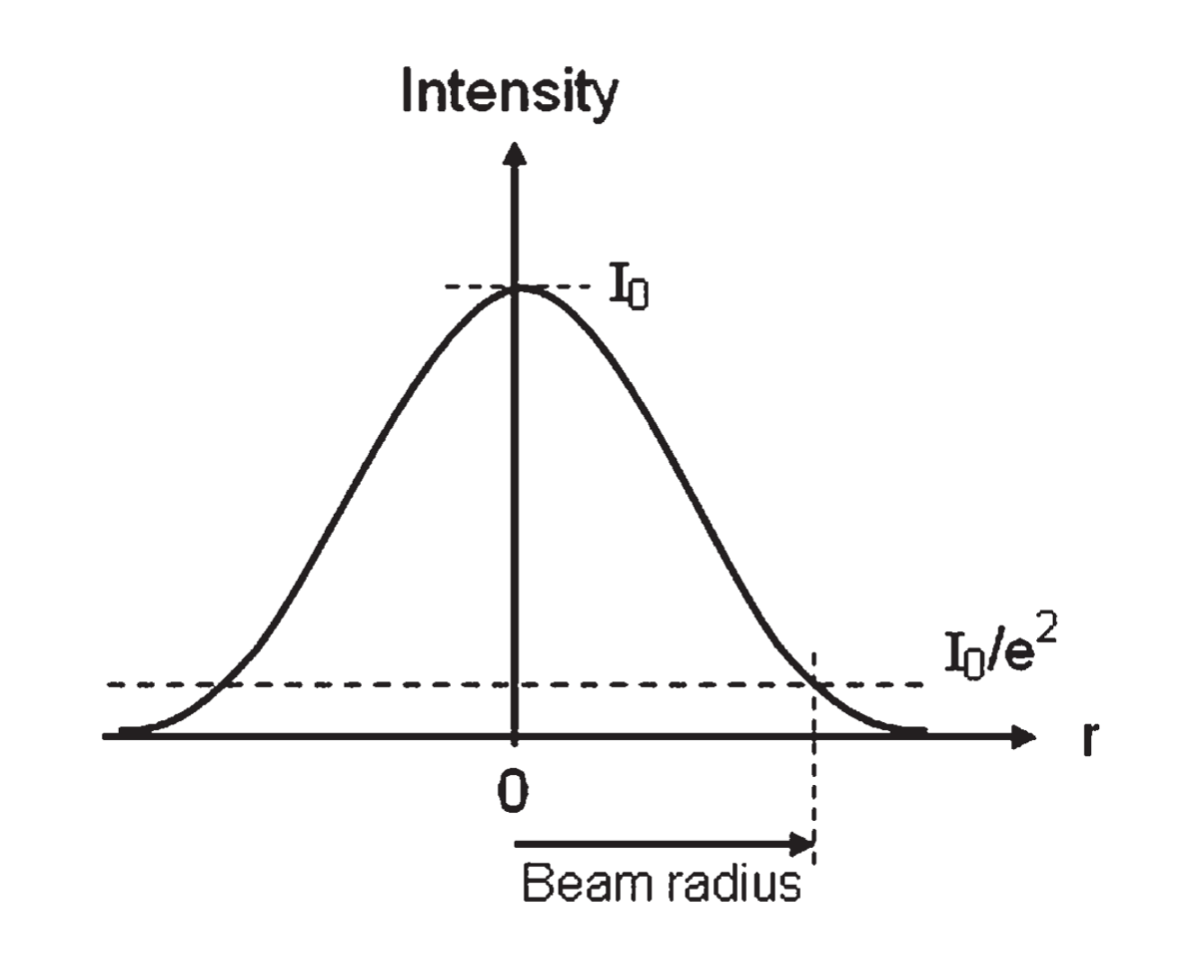
\includegraphics[scale=0.28]{Images/laserintensity.png}
    }
    
    \caption[Laser interactions and laser intensity.]{Schematic representation of physical interaction of absorption, reflection, transmission, refraction, and scattering between laser beam and material (a) \cite{katayama_fundamentals_2020}, and laser intensity schema (b).}
\end{figure}
For example, copper's absorptivity is about 50\% and 58\% for green and blue lasers, respectively. In other words, green and blue lasers are more advantageous in processing copper powder in terms of higher initial absorption than other laser typologies. As we will explore later, the electron beam transfers energy to the material through charge movement, while the laser beam operates as an optical device and hence it is more sensitive to the behaviors illustrated in Fig. \ref{fig:laserintera}. Indeed, the metal specimen is highly reflective and opaque. This is also the reason why the electron beam penetrates deeper into the metallic powder compared to the laser beam. The intensity of the laser emission varies as a function of the radius as 
\begin{equation}
    \label{eq:intensitylaser}
    I(r)=I_0\cdot e^{-2 \frac{r^2}{r_0^2}}
\end{equation}
and a schematic representation of density is shown in Fig. \ref{fig:laserintensity}.
The energy density of the laser beam is described by the equation
\begin{equation}
    \label{eq:energydensity}
    E_d = \frac{P}{h\cdot v \cdot d}
\end{equation}
where $E_d$ is the energy density (\unit{\joule/\milli\metre^3}), $P$ is the laser power (\unit{\watt}), $v$ is the laser scan speed (\unit{\milli\metre / \second}), $h$ is the hatch distance (\unit{\milli\metre}), $d$ is the layer thickness of the powder(\unit{\milli\metre}). For a more detailed description of heat transfer, please refer to the next section. The intensity of the laser beam's energy plays a crucial role in SLS because if it is not correctly calibrated, the final piece might exhibit porosities that compromise its mechanical features. Another critical parameter to consider during the SLS process is the duration of the laser pulse. As depicted in the Fig. \ref{fig:pulsipulsiocomepulsi} a prolonged laser pulse results in a broad heat zone, causing a shock wave that leads to an increased debris formation during the interaction that can interfere with new layers.
\begin{figure}
    \centering
    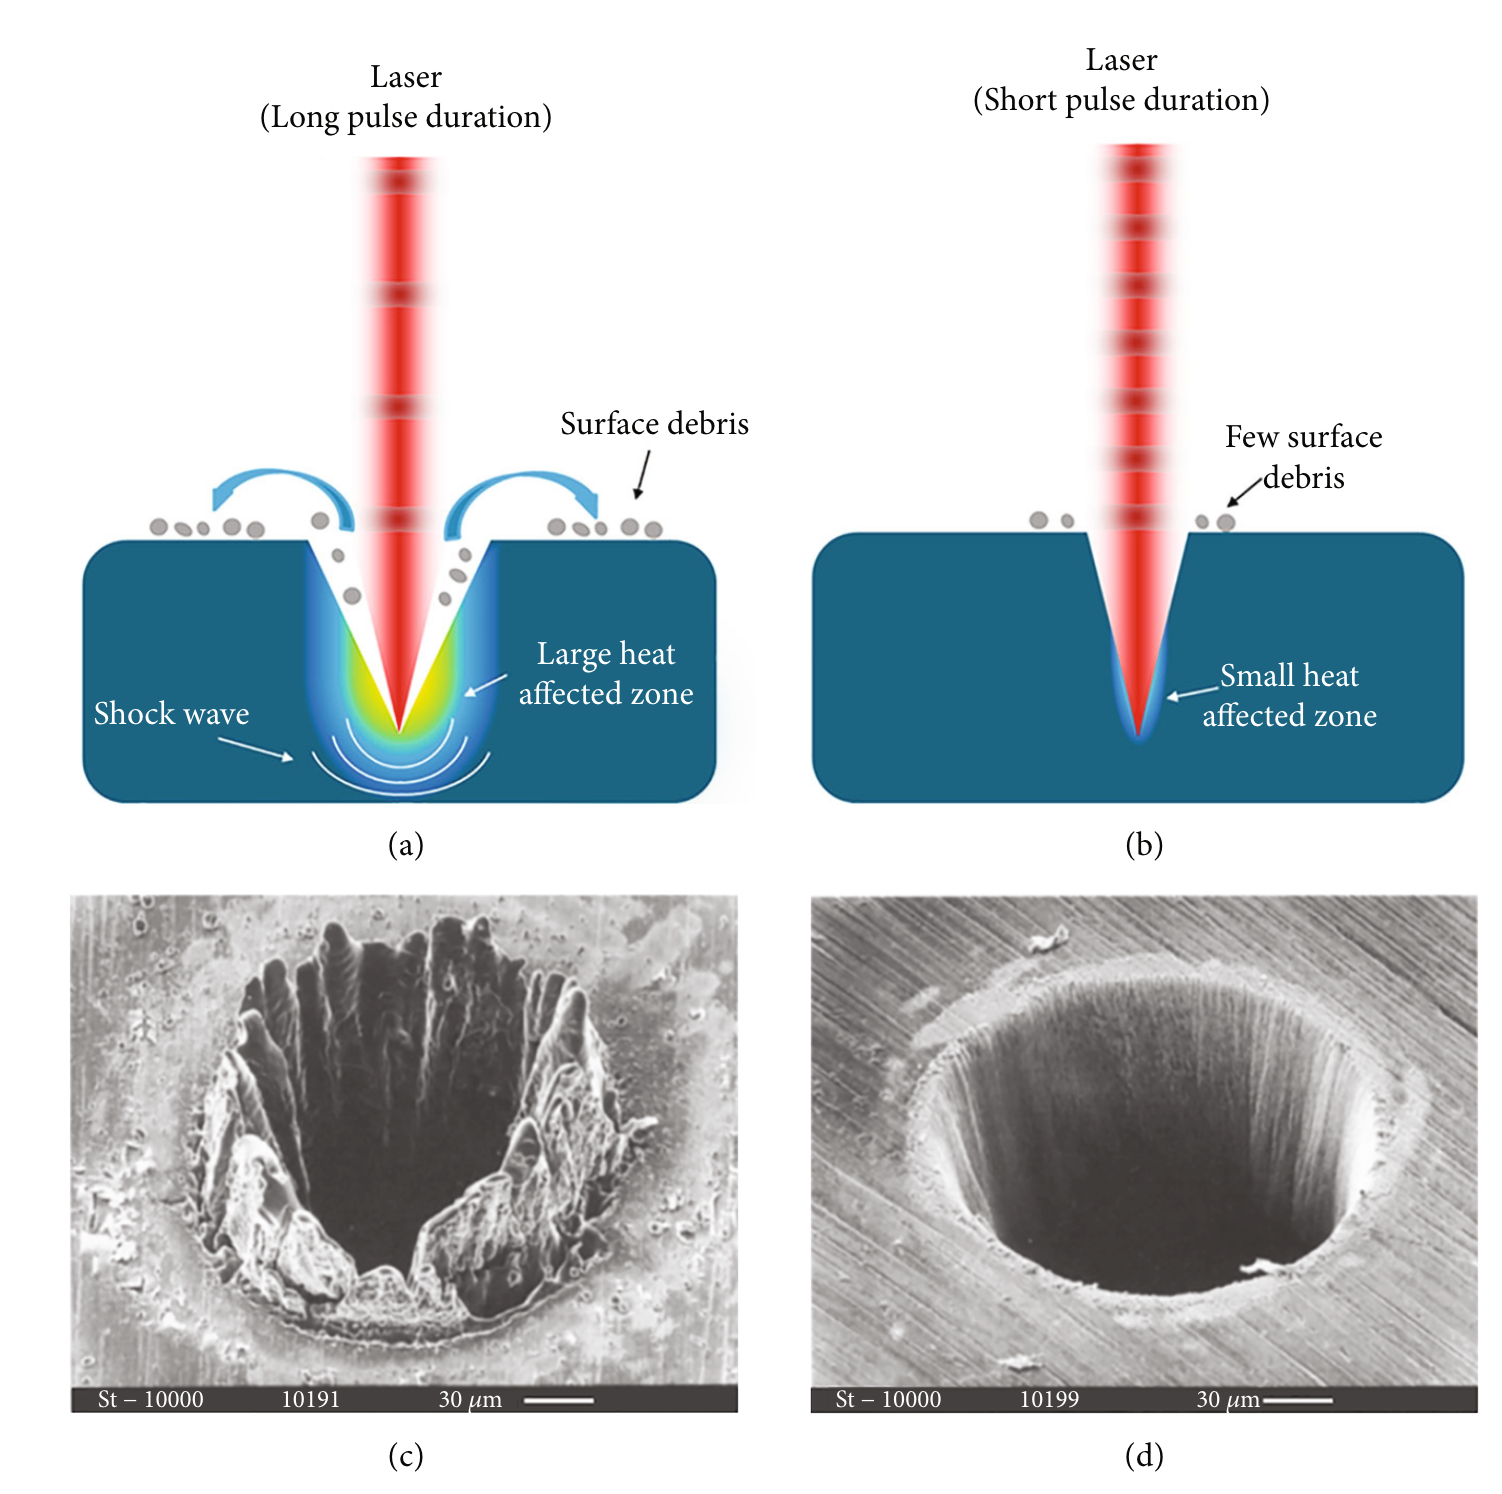
\includegraphics[scale=0.35]{Images/laserpulsing.png}
    \caption[Material absorptivity as function of wavelength.]{Schematic of laser interaction with materials under different pulse duration: (a) long pulse duration and (b) short pulse duration and respective holes fabricated on a steel foil by (c-d) \cite{lin_femtosecond_2021}.}
    \label{fig:pulsipulsiocomepulsi}
\end{figure}
For this reason, in recent years, there has been a shift towards using ultra-short pulse lasers. A schematic representation of one of this laser can be seen in Fig. \ref{fig:duripoco}. The laser in the figure is called "femtosecond laser" and is employed in manufacturing contexts such as precision processing or correction of semiconductors and liquid crystals, processing of transparent materials like glasses and sapphires, production of waveguide tubes for optical communication, drilling of engine components for cars and aircraft, among other applications \cite{katayama_fundamentals_2020}.
\begin{figure}
    \centering
    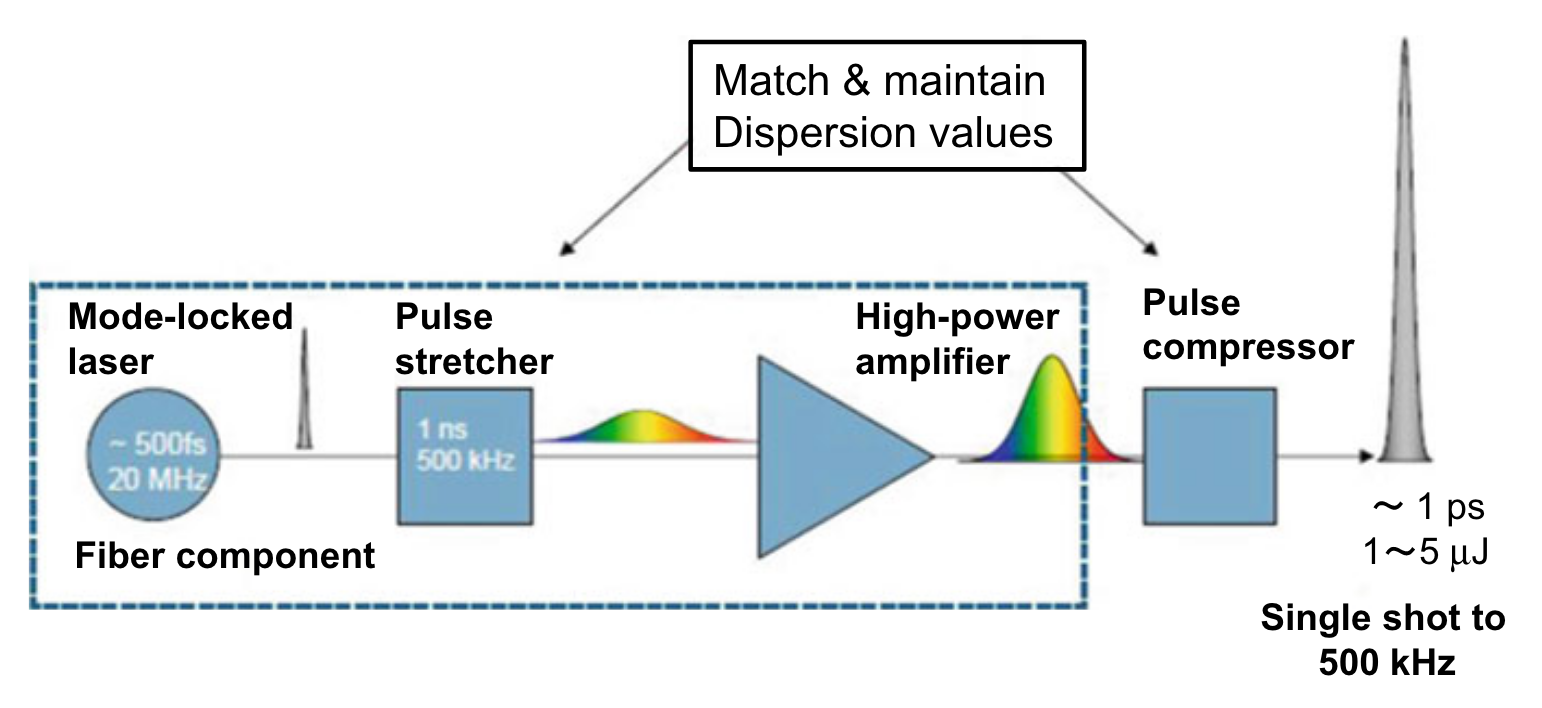
\includegraphics[scale=0.4]{Images/duripoco.png}
    \caption[Ultrashort pulse laser.]{Emission mechanism of ultrashort pulse laser \cite{katayama_fundamentals_2020}.}
    \label{fig:duripoco}
\end{figure}
\subsubsection{Heat transfer}
\label{sssec:heattransfer}
The heat and mass related events in SLS are influenced by both heat and mass movement. Laser heating is extremely rapid due to the fast scanning laser velocities. In a closed system, with respect to the first law of thermodynamics, the energy balance equation is formulated as follows \cite{bouabbou_understanding_2022}:
\begin{equation}
    \label{eq:tutteQ}
    Q_L = Q_C + Q_{CV} + Q_R,
\end{equation}
where $Q_L$, $Q_C$, $Q_{CV}$ and $Q_R$ respectively are the laser heat flux quantity, conduction, convection and radiation heat quantities. Recalling that only $Q_C$ will contribute to the melting process. Thus, some of the heat applied on the powder bed will be lost in the form of heat convection and radiation. \\
To describe the heat conduction, we can use Fourier's law:
\begin{equation}
    \label{eq:nonsiecapitouncazzo}
    \frac{\delta}{\delta x}\left(k \frac{\delta T}{\delta x}\right)+\frac{\delta}{\delta y}\left(k \frac{\delta T}{\delta y}\right)+\frac{\delta}{\delta z}\left(k \frac{\delta T}{\delta z}\right)+\dot{q} =\rho C_p \frac{\delta T}{\delta t}
\end{equation}
where $T$ (\unit{\kelvin}) is the temperature, $k$ (\unit{\watt.\metre^{-1}.\kelvin^{-1}}) is the thermal conductivity, $\dot{q}$ (\unit{\watt.\metre^{-3}}) is the rate of which the heat is applied to the system, $r$ (\unit{\kilo\gram.\metre^{-3}}) is the material density, $C_p$ (\unit{\joule. \kilo\gram^{-1}.\kelvin^{-1}}) is the specific heat and $t$ (\unit{\second}) is the interaction time between laser beam and powder particles.

\subsubsection{Optical Fiber Laser}
\label{sssec:fiberlaser}
One of the most common types of lasers used in SLS is the fiber optic laser \cite{milewski_additive_2017}. A diode is a semiconductor component acting like an unidirectional electric current gate. It permits current to pass effortlessly in one direction but significantly hinders its flow in the opposite one. Diodes have a polarity characterized by its anode (positive terminal) and cathode (negative terminal). Typically, diodes conduct current only when a positive voltage is supplied to the anode. In a laser diode (LD), an electric current is channeled directly through a dual hetero-junction structured semiconductor from the external side. When electrons recombine with positive holes at the active layer located between the n-type and p-type semiconductor zones, as shown in Fig. \ref{fig:np}, there is the emission of light beam.
\begin{figure}
    \centering
    \subfloat[\label{fig:np}]{
        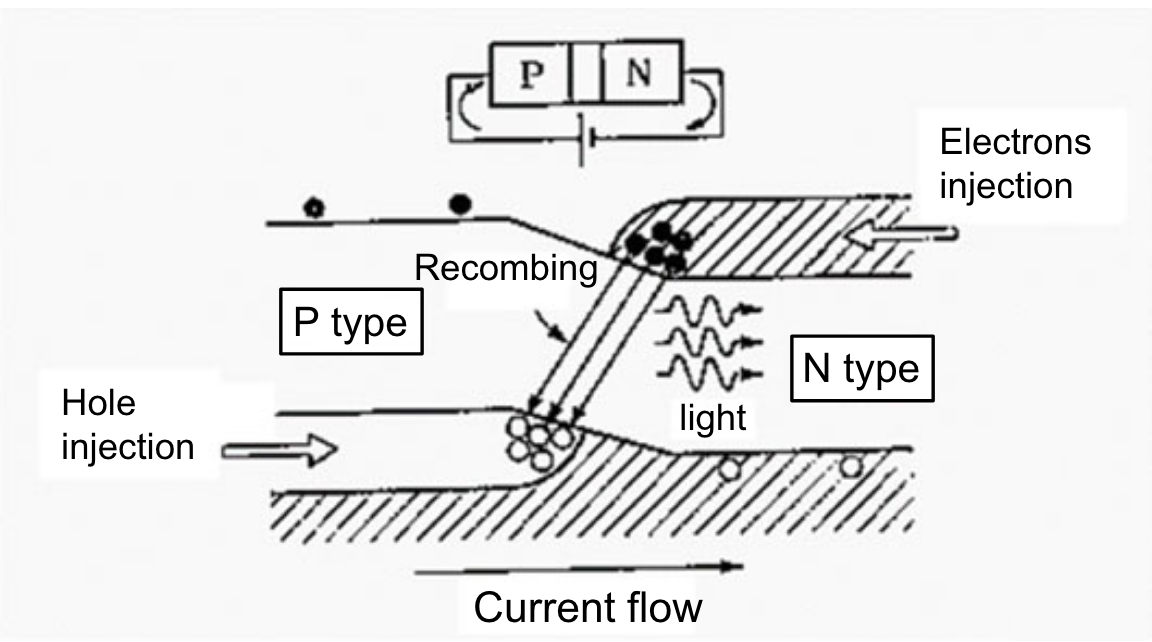
\includegraphics[scale=0.35]{Images/np.png}}
    \qquad
    \subfloat[\label{fig:detailedfiber}]{
        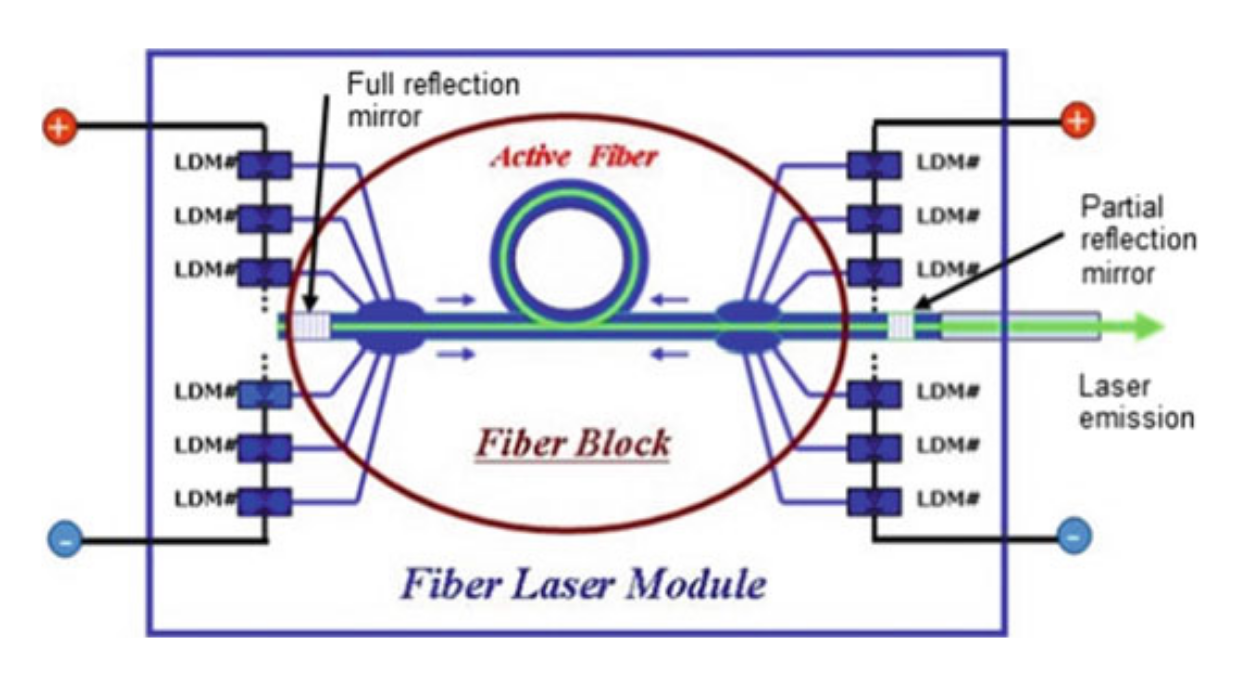
\includegraphics[scale=0.35]{Images/detailedfiber.png}}
    \caption[Laser diode and fiber laser.]{Emission mechanism of laser diode (a) and a detailed fiber laser schema (b) \cite{katayama_fundamentals_2020}.}
    
\end{figure}
In fiber lasers, the beam is emitted by an LD pumping and a fiber of high purity \ce{SiO2} quartz glass doped with \ce{Yb^3+} rare earth element. The diameter of the fiber is about \numrange[range-phrase=--]{10}{20}\unit{\micro\metre}. In this laser technology, optical pump diodes are coupled to an active laser fiber that has a unique reflective coating and Bragg gratings that reflect the laser light back and forth along the length of the fiber to create a coherent beam of light at the output of the laser \cite{milewski_additive_2017}. In Fig. \ref{fig:detailedfiber} we can see full reflection mirror and partial reflection mirror installed next to the fiber. This also means that the laser beam adjustment is not needed, which means easier handling of the system. Combining multiple laser modules using a beam combiner for a more powerful laser is also possible. We can use additional optical fibers to deliver and contain the light energy, providing a robust, flexible, and fully enclosed beam path for beam delivery \cite{milewski_additive_2017}. Fiber laser has many \textit{advantages} such as high beam quality, the fact they are small and lightweight, high intensity (which allows higher scan speed) and high efficiency (cost decreasing), long-distance delivery, and require basically no maintenance. 
\subsection{Electrons-Matter Interaction}
\label{subsec:ebminter}
According to \citeauthor{schultz_h_electron_1994} (1994), while the physical characterization of electron beams has been recognized since the 1960s, the microscopic processes are such that they remain without a comprehensive quantitative explanation also nowadays. However, a comprehensive explanation of electrons properties and their interaction with matter was given by \citeauthor{krumeich_properties_2015} (2015).
\subsubsection{What is an Electron?}
\label{sssec:electron}
An electron is a fundamental subatomic particle that carries a negative electric charge and is one of the primary constituents of atoms. As explained in Section \ref{subsec:ebm} the electron beam is made of electrons generated through the thermionic effect with a metallic filament, typically tungsten or tantalum. At the cathode, an accelerating voltage $V$ is applied, causing electrons acceleration till velocity $v$. As explained in \citeauthor{krumeich_properties_2015} (2015), we can write the equation for kinetic energy associated to an electron as 
\begin{equation}
    \label{eq:energyelectron}
    E  = e\cdot V = \frac{1}{2}mv^2
\end{equation}
Given the fact that electron mass is \SI{9.109e-31}{\kilo\gram}, electron charge is \SI{-1.602e-19}{\coulomb} and that a common voltage for EBM application is \SI{60}{\kilo\volt}, from \ref{eq:energyelectron} we find that electron velocity is
\begin{equation}
\label{eq:velocityelectron}
v=\frac{\sqrt{2\cdot e\cdot V}}{m}
\end{equation}
which is approximately \num{1.453e8} \unit{m/s} (about half the speed of light). Recalling the dualism wave-particle of the electron, we can use De Broglie equation to compute the wavelength of the electron beam \cite{krumeich_properties_2015}:
\begin{equation}
\label{eq:wavelength}
    \lambda = \frac{h}{\sqrt{2\cdot m \cdot e \cdot V}}
\end{equation}
where $h=$\SI{6.62607015e-34}{\joule.\second} is Planck constant. In case of a voltage higher than \SI{300}{\kilo\volt}, it's necessary to include a term that accounts for the relativistic nature of mass in \ref{eq:wavelength}, as the electron's speed would approach the speed of light.
\subsubsection{Magnetic Lenses in EBM}
\label{sssec:magneticlens}
In EBM, electromagnetic lenses control the beam emission. As the beam passes through these lenses, the astigmatic lenses adjust the shape of the electron beam spot, the focus coil changes the spot size, and the deflection coil moves the beam along the x and y axes.
\begin{figure}
    \centering
    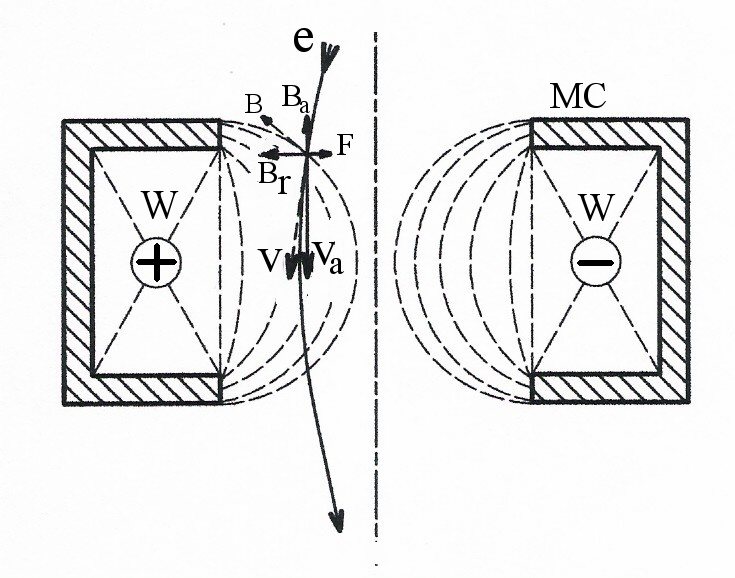
\includegraphics[scale=0.7]{Images/Magnetic_lens.jpg}
    \caption[Magnetic lens.]{Forces schema when an electron beam pass through magnetic lens \cite{wikipedia_magnetic_2023}.}
    \label{fig:magneticlens}
\end{figure}
The force $\mathbf{F}$ which an electron of charge $-e$ experiences when traveling with a velocity $\mathbf{v}$ due to a magnetic field $\mathbf{B}$ is given by Lorentz's law:
\begin{equation}
    \mathbf{F} = -e\cdot \left( \mathbf{v} \times \mathbf{B}\right)
\end{equation}
We can decompose the magnetic field into a radial component $\mathbf{B}_R$ and an axial component $\mathbf{B}_L$. The initial direction of the electron is parallel to the axis. Thus, it is subjected to the radial component $\mathbf{B}_R$ only, which is responsible for an orthogonal force to $\mathbf{v}$. Hence, electrons start rotating. When they start spinning, they are subject to the axial field of the magnetic field too, which results in a reducing radius spiraling trajectory that converges the beam towards the target.
\subsubsection{Electrons Interaction}
\label{sssec:electroninteractions}
\begin{figure}
    \centering
    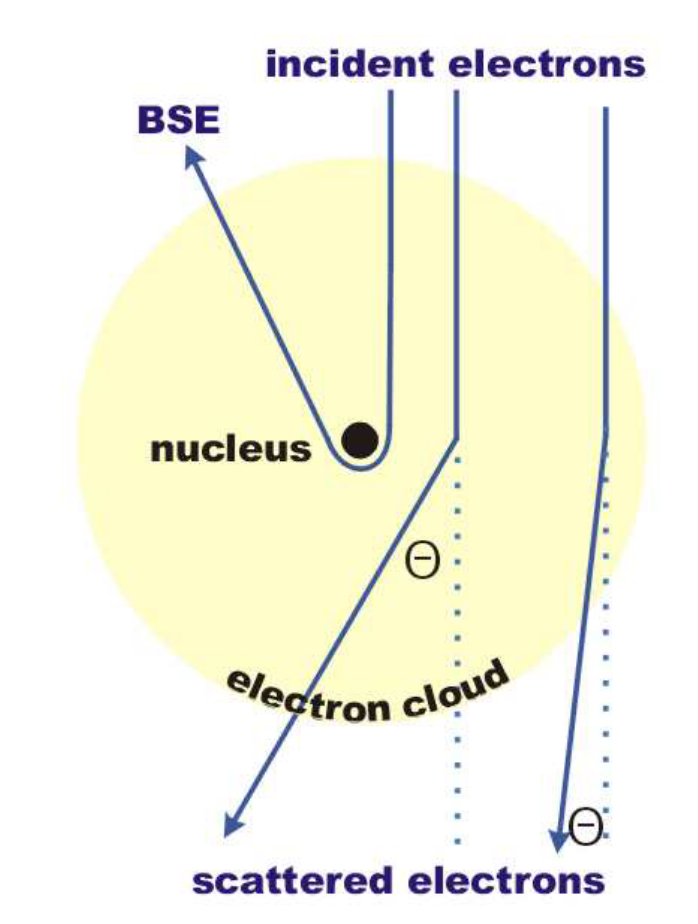
\includegraphics[scale=0.35]{Images/electrons.png}
    \caption[Scattering and backscattering of an electron.]{Scattering and backscattering effect of an incident electron inside the electron cloud of an atom \cite{krumeich_properties_2015}.}
    \label{fig:electronsscattering}
\end{figure}
As explained in \citeauthor{korner_additive_2016} (2016), we can distinguish two interaction types between electrons and matters, defined on the basis of transferred energy quantity. 
\paragraph{Elastic interactions} The electron's energy remains constant: when electrons delve into the surface, they engage as negatively charged entities with the metal's negative field and the positive charge from the nucleus's protons. Electrons can be rerouted on a different path without losing kinetic energy (known as elastic scattering). After several interactions, these deflected electrons might sometimes exit from the metal. This phenomenon is called backscattering. In Fig. \ref{fig:electronsscattering}, there is a representation of all the possible interactions between an electron and an atom nucleus. This event occurs because of the Coulomb interaction, which happens when a negatively charged entity (electron) comes close to a positively charged one (nucleus). Coulomb force is described by the equation:
\begin{equation}
    \label{eq:coulomb}
    F=\frac{Q_1\cdot Q_2}{4\pi \varepsilon_0 r^2}
\end{equation}
where $r$ is the distance between the charges $Q_1$ and $Q_2$ and $\varepsilon_0=$ \SI{8.854e-12}{\farad / \metre} is the dielectric constant. The backscatter phenomenon is determined by material characteristics and the angle at which the beam hits the metal surface. See Fig. \ref{fig:backscattering}. It represents an energy deduction from the melting procedure. Indeed, if an electron exits the material, it cannot transfer energy to the material itself. So, for process efficiency, we have to avoid these interactions. The backscattering effect is directly proportional to the atomic number $Z$ of the material of the powder, specifically $Z^2$.
\begin{figure}
    \centering
    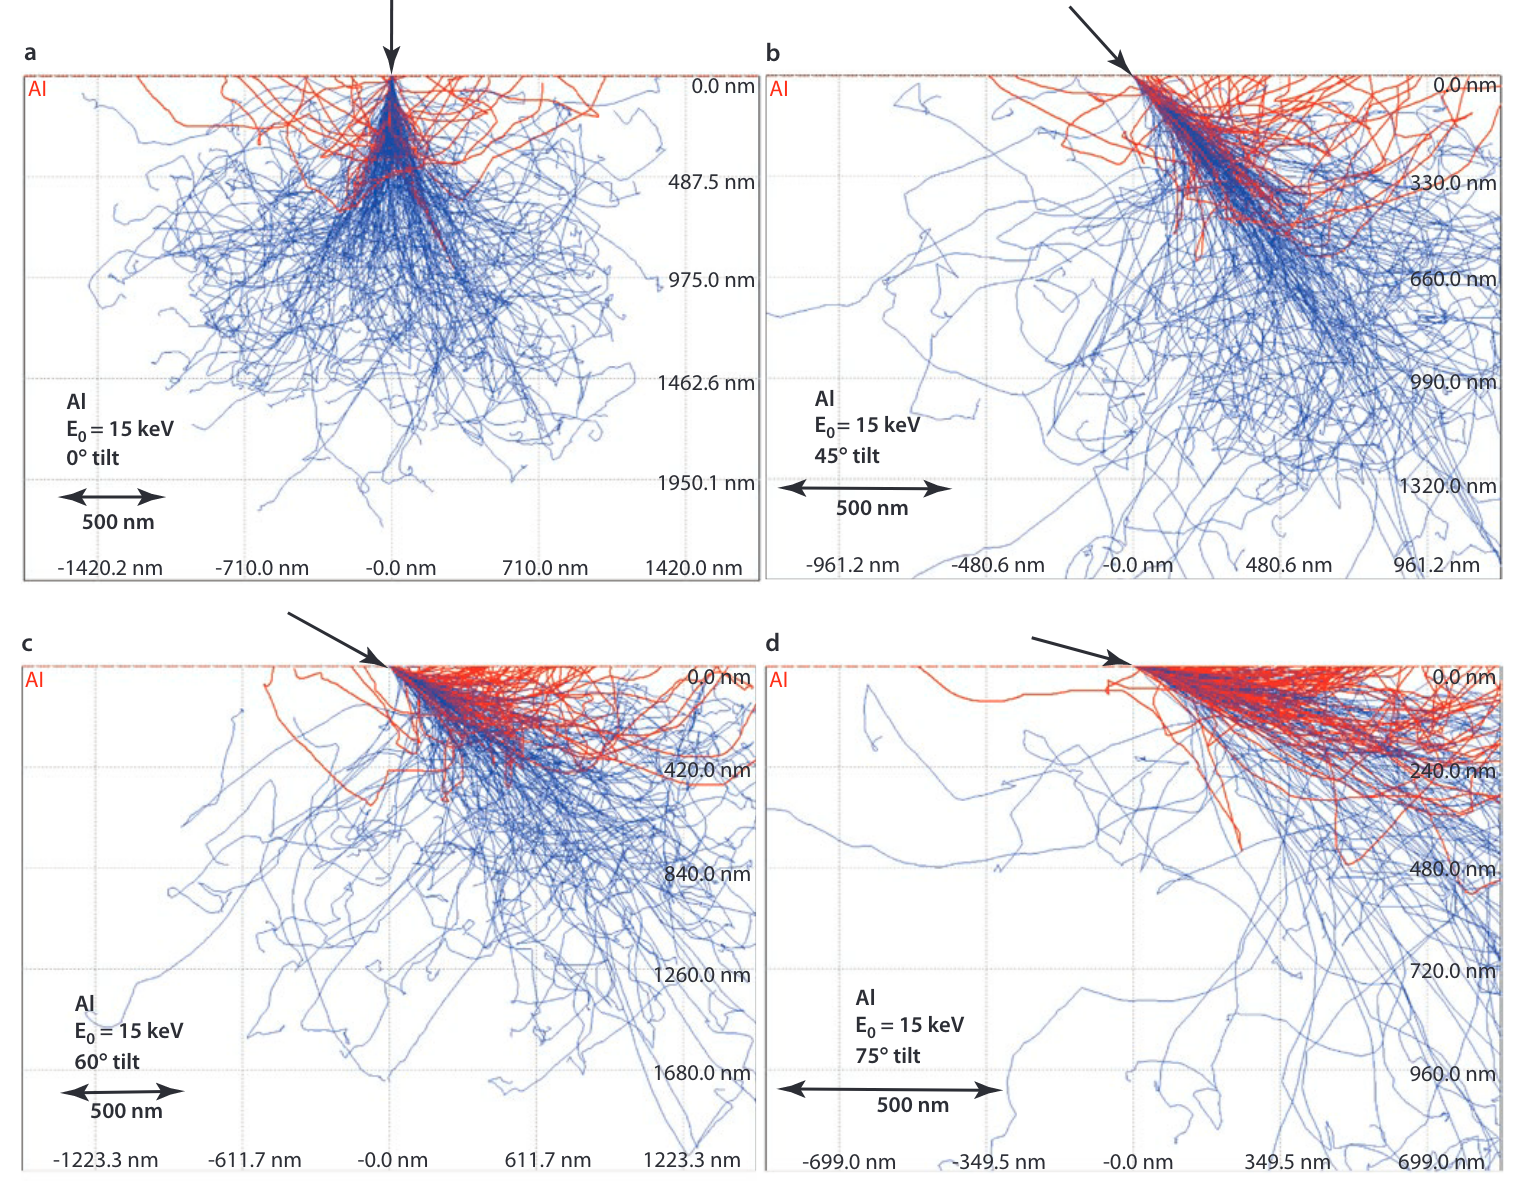
\includegraphics[scale=0.4]{Images/backscattering.png}
    \caption[Backscattering of an electron at different angles.]{Montecarlo simulation for an aluminum specimen hit by an electron beam at different angles, \ang{0}, \ang{45}, \ang{60}, \ang{75} respectively \cite{goldstein_scanning_2018}. In red, backscattered electrons.}
    \label{fig:backscattering}
\end{figure}
A fine and as spherical as possible powder is essential to reduce the backscattering effect caused by the incidence angle. In EBM processes, the more spherical the particles are, the more we can assume that the electron beam will strike the particle surface perpendicularly. We can see in Fig. \ref{fig:rotondette} why.
\paragraph{Inelastic Interactions:} In inelastic interactions, the energy of the electrons diminishes. The energy imparted to the sample results in the heating of the metal and its corresponding melting. These interactions cause the release of certain emissions, detailed below \cite{krumeich_properties_2015, goldstein_scanning_2018}:
\begin{itemize}
    \item \textbf{Inner-shell ionization :} The energy is passed to an inner electron, which is adequate to eject it from the atom. This results in an unstable atom configuration, leading to the release of X-rays or an Auger electron. \emph{X-rays} are produced when an inner electron is released into the vacuum, and an electron from the valence shell descends to occupy the void left by the electron from a deeper level. On the other hand, an \emph{Auger electron} is produced when the core electron, stimulated by the electron beam's energy, is expelled into the vacuum. Another electron from a higher level occupies the left space, which then radiates energy to a closer electron until it is released into the chamber. That's why, in an EBM 3D printer, it is crucial to have a shield to protect operators from X-rays.
    \item \textbf{Braking radiation:} The electron that enters the atom slows down due to its interaction with the positively charged nucleus. The subsequent reduction in energy is released as X-rays. The material completely absorbs X-rays of lower energy, while X-rays of higher energy are released in the printing chamber.
    \item \textbf{Secondary electron:} Electrons within the valence band require minimal energy to surpass the potential barrier, and various electron-matter interaction mechanisms can provide this energy. This can cause the release of these electrons in the printing chamber. The inert gas flow in the chamber removes these electrons from the powder bed since they can interfere with the printing process.
    \item \textbf{Cathodoluminescence:} when an electron from the valence band rises to the conduction band, a vacancy is created in the valence band. Another electron descending from the conduction band occupies this vacancy, which releases a photon. This phenomenon is responsible for the characteristic light produced when the electron beam hits the metal powder in EBM. 
    \item \textbf{Plasmon:} an electron moving through the collection of electrons in the valence band can cause a disturbance, leading to a collective vibration of the free electrons. This interaction is prevalent in metals but can also occur in any substance with free electrons. This phenomenon is responsible for the creation of plasma oscillation.
    \item \textbf{Phonons:} Phonons are understood as the collective oscillations of atoms within a crystal lattice, resulting from inelastic engagements with the electron beam. When an atom initiates this vibrational movement, it conveys this activity throughout the lattice, impacting a significant volume. Phonons are the only ones responsible for the melting of metal powders. Other products are undesirable or even accountable for side effects during the printing process.
\end{itemize}
\begin{figure}
    \centering
    \subfloat[\label{fig:rotondette}]{
        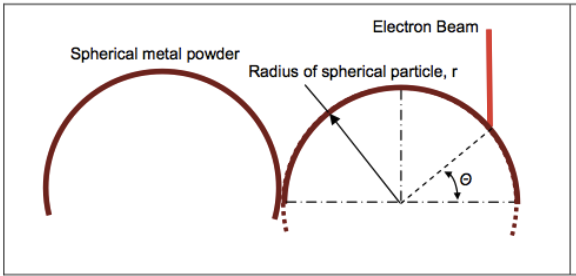
\includegraphics[scale=0.65]{Images/EBMparticles.png}
    }
    \qquad
    \subfloat[\label{fig:unsaccodiroba}]{
        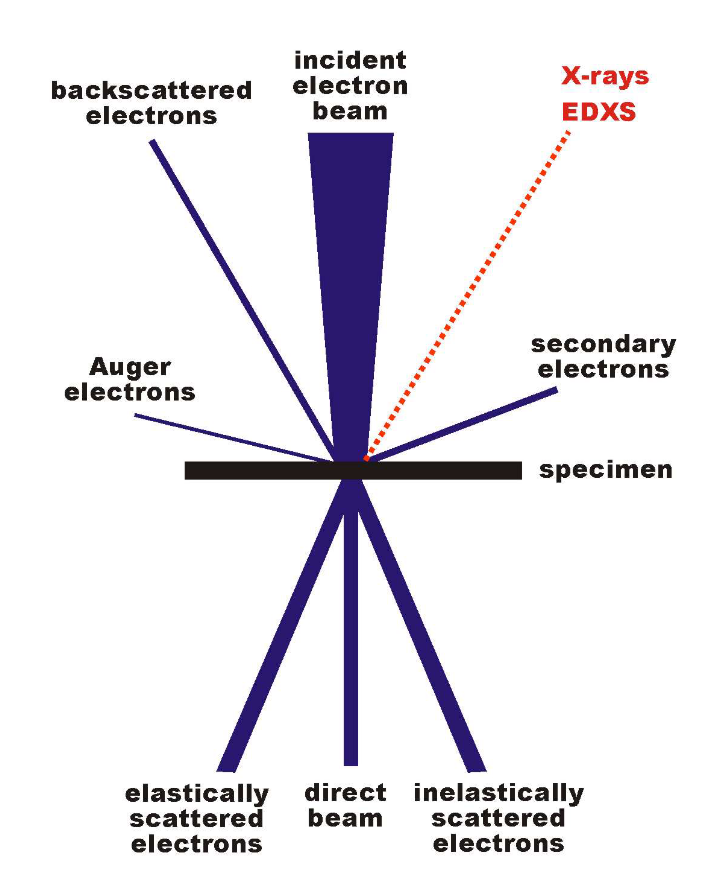
\includegraphics[scale=0.35]{Images/Screenshot 2023-08-21 at 11.42.27.png}
    }
    \caption[Laser interactions and laser intensity.]{Electron beam interaction with spherical powder particles (a) and Product from the interaction between an electron and a metal specimen (b) \cite{tushar_ramkrishna_mahale_electron_2009, krumeich_properties_2015}.}
\end{figure}
In Fig. \ref{fig:unsaccodiroba}, there is a schematic representation of the products resulting from the collision between an electron and a metal specimen.
% <<< End of Energy Matter Interactions

%%%%%
%%%%%

% Applications of PBF Metal Additive Manufacturing >>>
\section{Applications of PBF Metal Additive Manufacturing}
\label{sec:examplesPBF}
One of the primary advantages of PBF processes is the capability to produce finished objects unattainable with traditional manufacturing systems. In this section, we'll explore some examples of how this technology can completely disrupt the production processes of metal manufacturing. The nozzle in Fig \ref{fig:nozzle} is one of the more famous, successful, and documented examples of additive manufacturing for metal. General Electrics designed it in 2015. With AM, GE could produce the new nozzle in a single piece rather than 20 pieces welded together. They were able to reduce weight by 25\%, and it was five times more durable and 30\% more cost-efficient \cite{amy_kover_transformation_2018}. GE Aviation has set the goal of 32,000 nozzles per year in whole production \cite{milewski_additive_2017}, opening this manufacturing process to large scale distribution. In 2015, NASA designed the first 3D-printed rocket nozzle made of copper. Within the combustion chamber, the propellant burns at temperatures exceeding \SI{3000}{\kelvin}. Hydrogen at temperatures just above \SI{100}{\kelvin} flows through over 200 intricately designed cooling channels to prevent it from melting. The chamber's top rim integrates cooling inlets. Thanks to this new rocket nozzle, costs were reduced by 50\% and manufacturing times were reduced by ten times \cite{tracy_mcmahan_nasa_2015}, opening the path to a more affordable and lean space industry. Fig. \ref{fig:piston} shows Porsche's application of PBF processes in the automotive sector. The company managed to print pistons by PBF for the 911 GT2 RS engine. These new pistons have achieved a temperature on the piston's o-ring that is \SI{20}{\degreeCelsius} lower than usual. This leads to an additional \SI{23}{\kilo\watt} power available. However, before we see large-scale production, we'll have to wait until at least 2030 \cite{roberto_baldwin_porsches_2020} according to Porsche's press release. AM is also being employed in the medical field, for example, in dentistry. Custom-fitted designs are transforming the traditional ways of fabricating items like crowns and dental implants. Advanced high-precision 3D printers, such as EOS M 100 DMLS, can print devices from Cobalt Chrome SP2 alloy, a medical-grade approved material in the medical field \cite{milewski_additive_2017}. Products with small batch sizes, high precision, and significant value, like these dental devices, are increasingly manufactured using these new technologies. The advantages of AM include the swift creation of tailor-made items for immediate application, such as implants, or indirect uses like drill guides and fixtures, all based on the patient's medical characteristics for a perfect fit. Moreover, the surface finish or porous structures offer better support for bone growth. In Fig. \ref{fig:skul} there is an example of a titanium skull implant.
\begin{figure}
    \centering
    
    \subfloat[\label{fig:nozzle}]{
        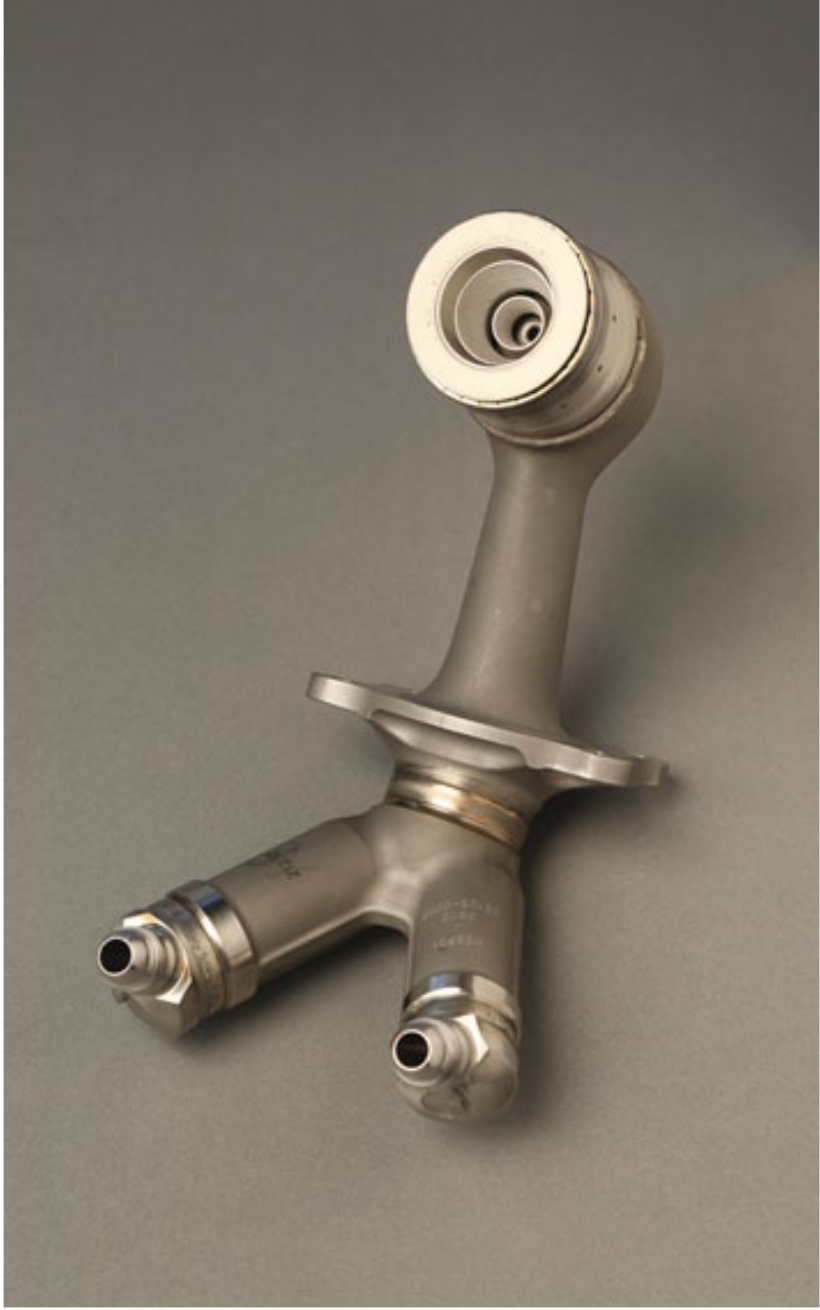
\includegraphics[scale=0.20]{Images/nozzle.png}
    }
    \qquad
     \subfloat[\label{fig:nozzlerocket}]{
        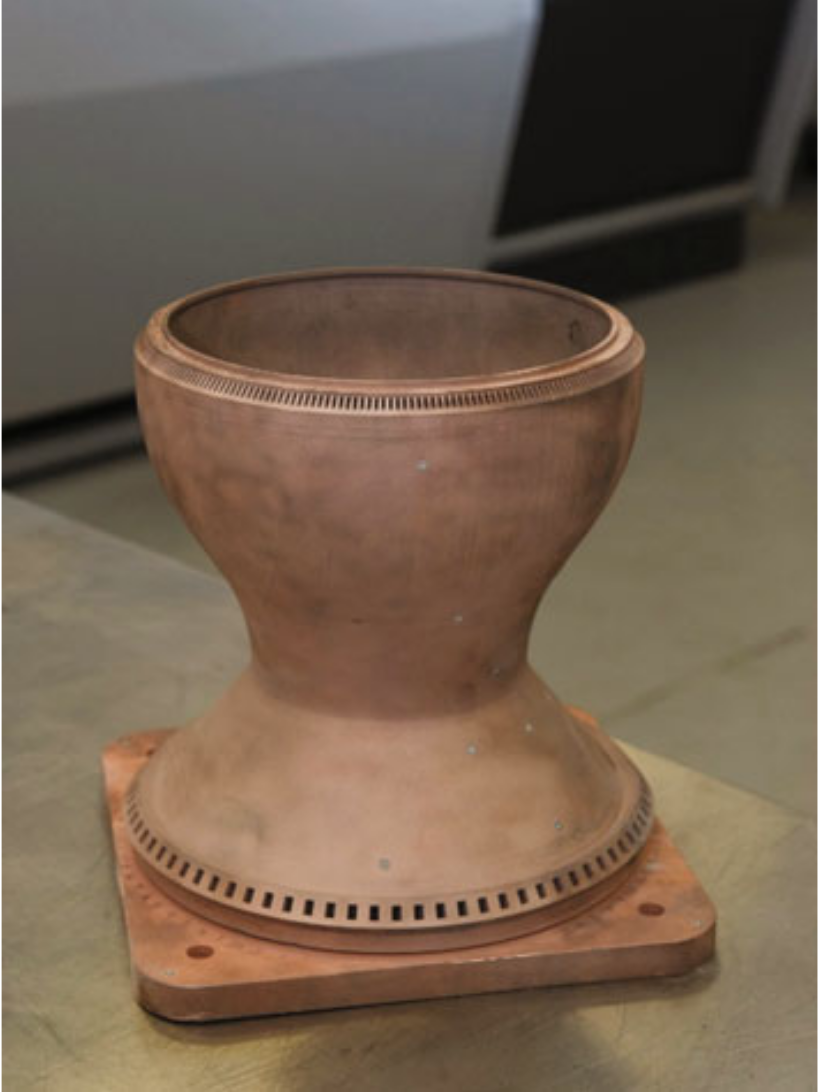
\includegraphics[scale=0.24]{Images/nozzlerocket.png}
    }
    \\
    \subfloat[\label{fig:piston}]{
        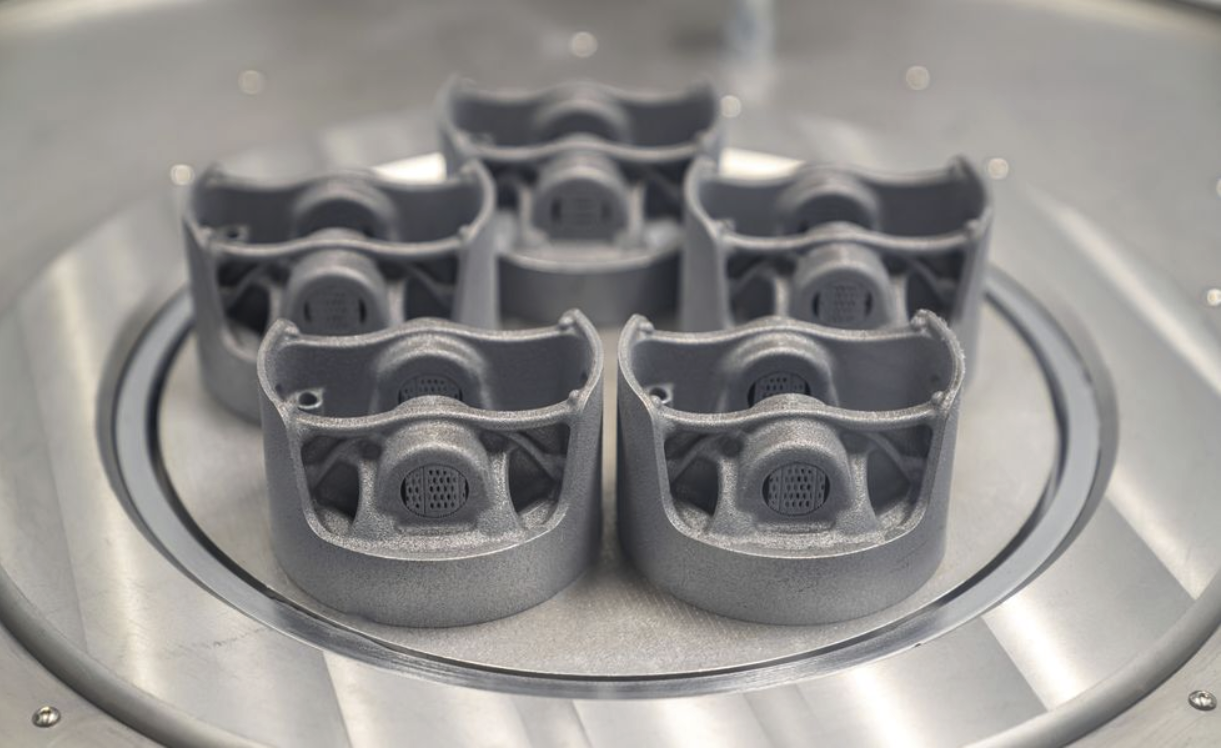
\includegraphics[scale=0.21]{Images/piston.png}
    }
    \qquad
    \subfloat[\label{fig:skul}]{
        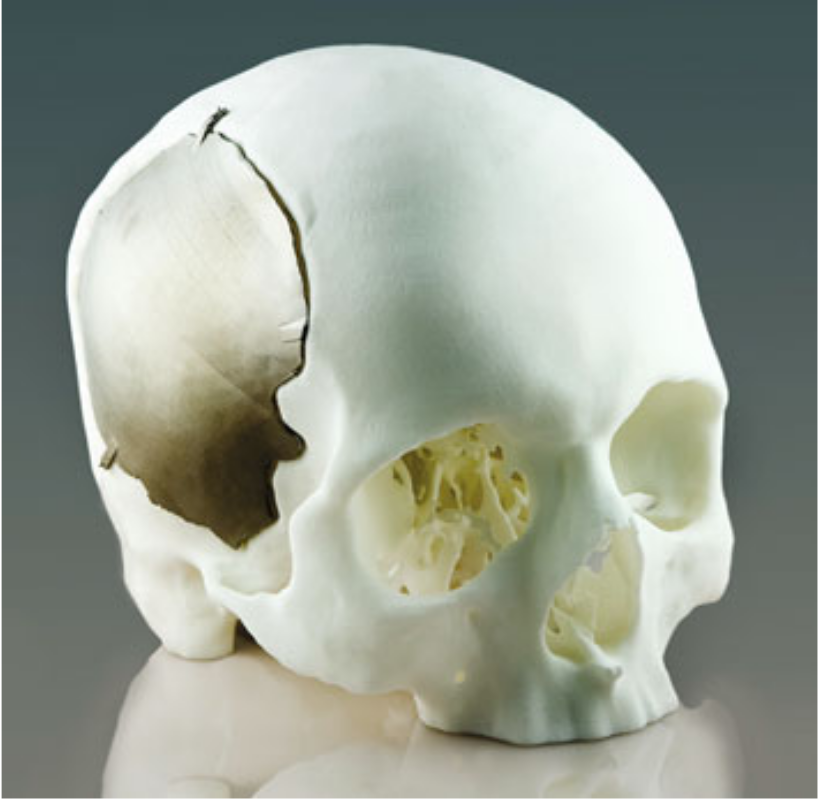
\includegraphics[scale=0.20]{Images/skull.png}
    }
    
    \caption[Examples of AM in metals.]{Examples of AM metal part: GE nozzle used in airplane turbines to mix fuel and air (a), a rocket nozzle in copper by NASA (b), Porsche engine pistons (c) and a titanium skull implant (d).}
    \label{fig:amexamples}
\end{figure}
\subsection{Lattice Structure and Cellular Material} \label{subsec:lattice}
A specific application of PBF processes is the printing of so-called lattice structures. According to ISO/ASTM 52900 \cite{organization_isoastm_2015}, \emph{lattice structure} are "three-dimensional geometric arrangement composed of connective links between vertices (points) creating a functional structure". Lattice structures are three-dimensional structures made up of different connected single elements called "cells" that can have different shapes designed to meet the desired mechanical features of the final object. These objects are distinguished by empty spaces within the structure. These structures can only be obtained thanks to layer-wise AM technologies. In recent years, the biomimicry technique has also spread in additive manufacturing. Biomimicry is a set of design techniques that allow us to take inspiration from nature to find solutions to engineering problems or to design functional components that can be used in engineering applications \cite{pathak_biomimicry_2019, du_plessis_beautiful_2019}. Over the past 3.8 billion years, nature has been able to find the most efficient way to develop functional solutions to evolutionary problems characterized by immovable constraints. Moreover, during the evolutionary process of species, nature has created nano, micro, and macro-structures that provide unique structural properties, adapting shape to function and using what is necessary to achieve the evolutionary goal. Indeed, one of life's principles explained in \citeauthor{baumeister_biomimicry_2011} (2011) states \textit{"Life integrates and optimizes these strategies to create conditions conducive to life"}. Therefore, it concerns creating new multi-functional structures with unique characteristics, optimizing materials, and reducing waste. Engineers have always been fascinated by cellular materials, evident from the first reference to the idea that structure could influence a material's functional characteristics and behavior, which Robert Hooke made in 1665 \cite{l_gibson_cellular_2010}. Only in recent years, thanks to the computational power of CAD softwares, it has been possible to experiment with the mechanical characteristics of 3D-printed lattice structures. Cellular materials are used mainly for their mechanical characteristics.
\begin{figure}
    \centering
    \subfloat[\label{fig:beehive}]{
        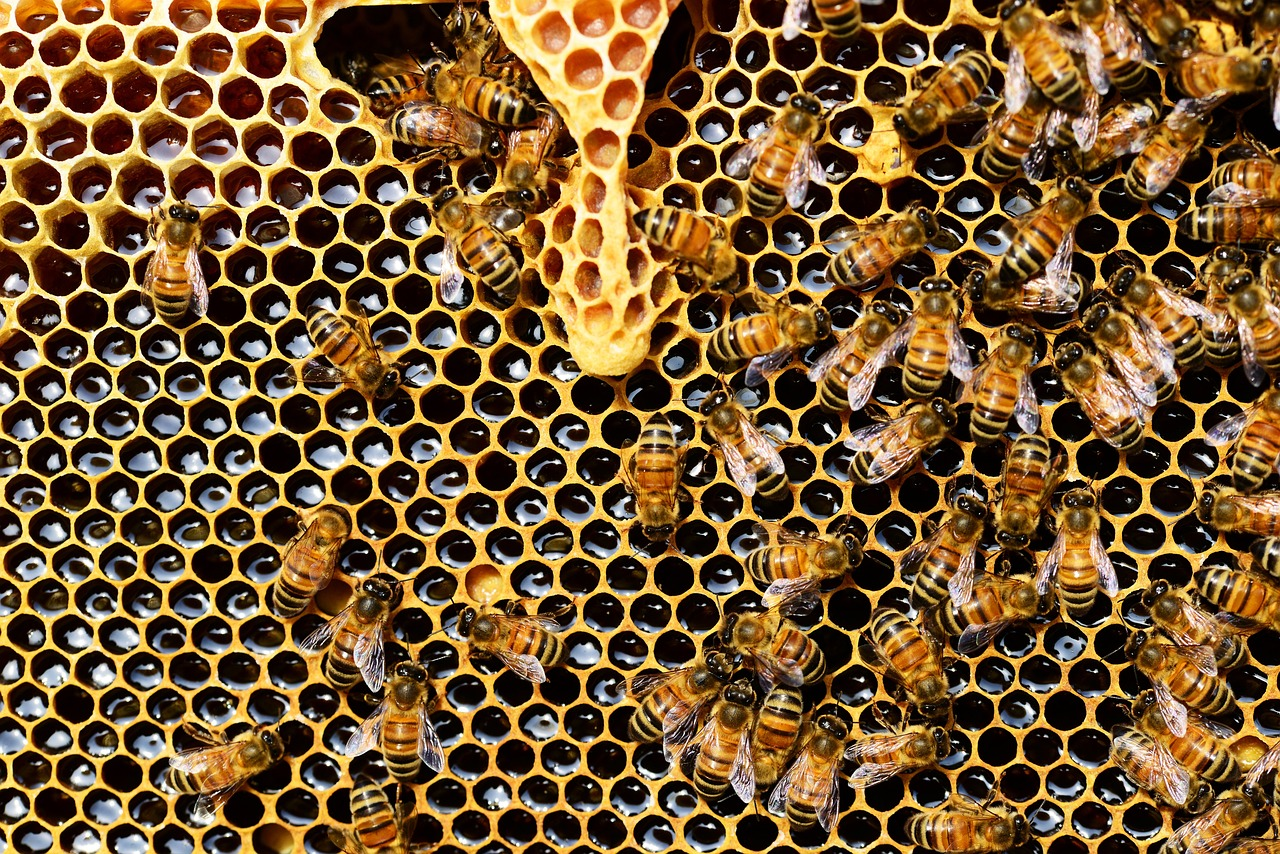
\includegraphics[scale=0.15]{Images/honey-bees-337695_1280.jpg}
    }
    \quad
    \subfloat[\label{fig:beelattice}]{
        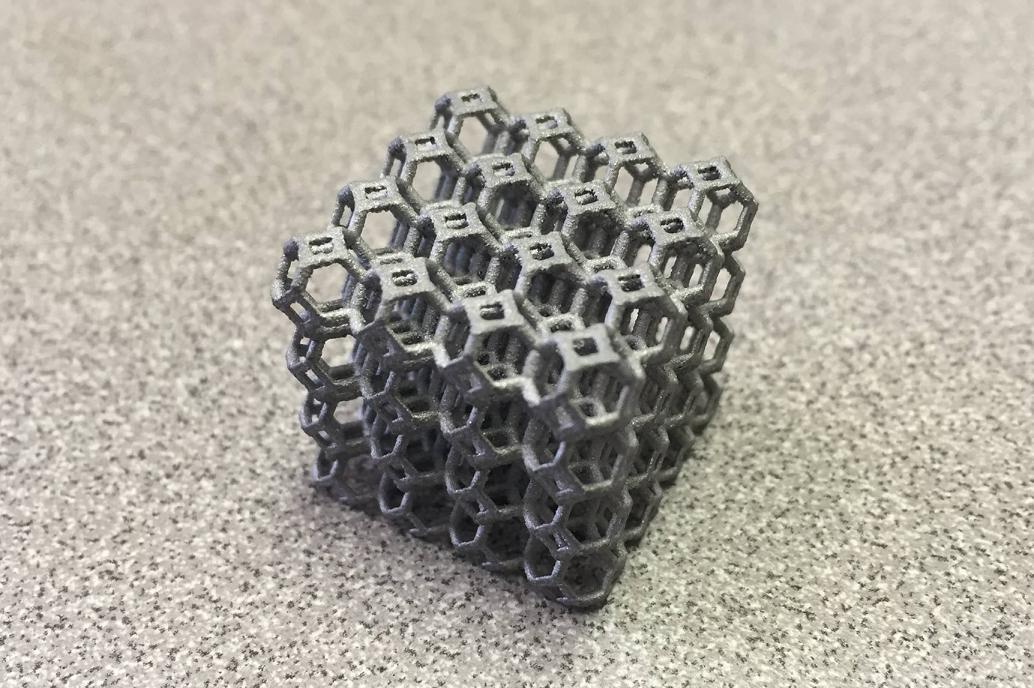
\includegraphics[scale=0.186]{Images/lattice1b.jpg}
    }
    \caption[Bio-inspiration design.]{An example of bio-inspiration design: from a beehive (a) to a lattice structure (b).}
    \label{fig:bioinsp}
\end{figure}
Just think that the aluminum cube in Fig. \ref{fig:beelattice} was printed using only \SI{3.9}{g} of material and can support a weight of \SI{408}{Kg}, which means it can withstand a stress 100,000 times its weight \cite{noauthor_3d_2014}. If we want to provide a more rigorous framework for classifying the applications of lattice structures in engineering, we can refer to the one proposed by \citeauthor{mcnulty_framework_2017}. According to this framework, cellular structures in nature exist primarily for three reasons:
\begin{itemize}
    \item \textbf{3D space-filling structures} may be the reason that most closely links the use of cellular structures in nature with AM, the need to confer strength to the structure while limiting its weight. Examples of this are the beehive, whose structure provides it with High specific stiffness under self-weight;
    \item \textbf{Surface structures}, enable surfaces to gain specific functional characteristics. For example, veining on the underside of the Amazon water lily leaf allows the leaf to gain excellent mechanical resistance, or the pomelo skin, with its open-cell structure, enables the fruit to resist impacts;
    \item \textbf{Cylindrical structures}: there are also examples of the use of cellular materials to confer particular characteristics to cylindrical structures (often hollow structures) that would otherwise be too fragile. For example, hedgehog quills have a particular internal structure that confers ovalization and buckling resistance to the quill.
\end{itemize}

\begin{figure}
    \centering
    \subfloat[\label{fig:heatexchanger}]{
        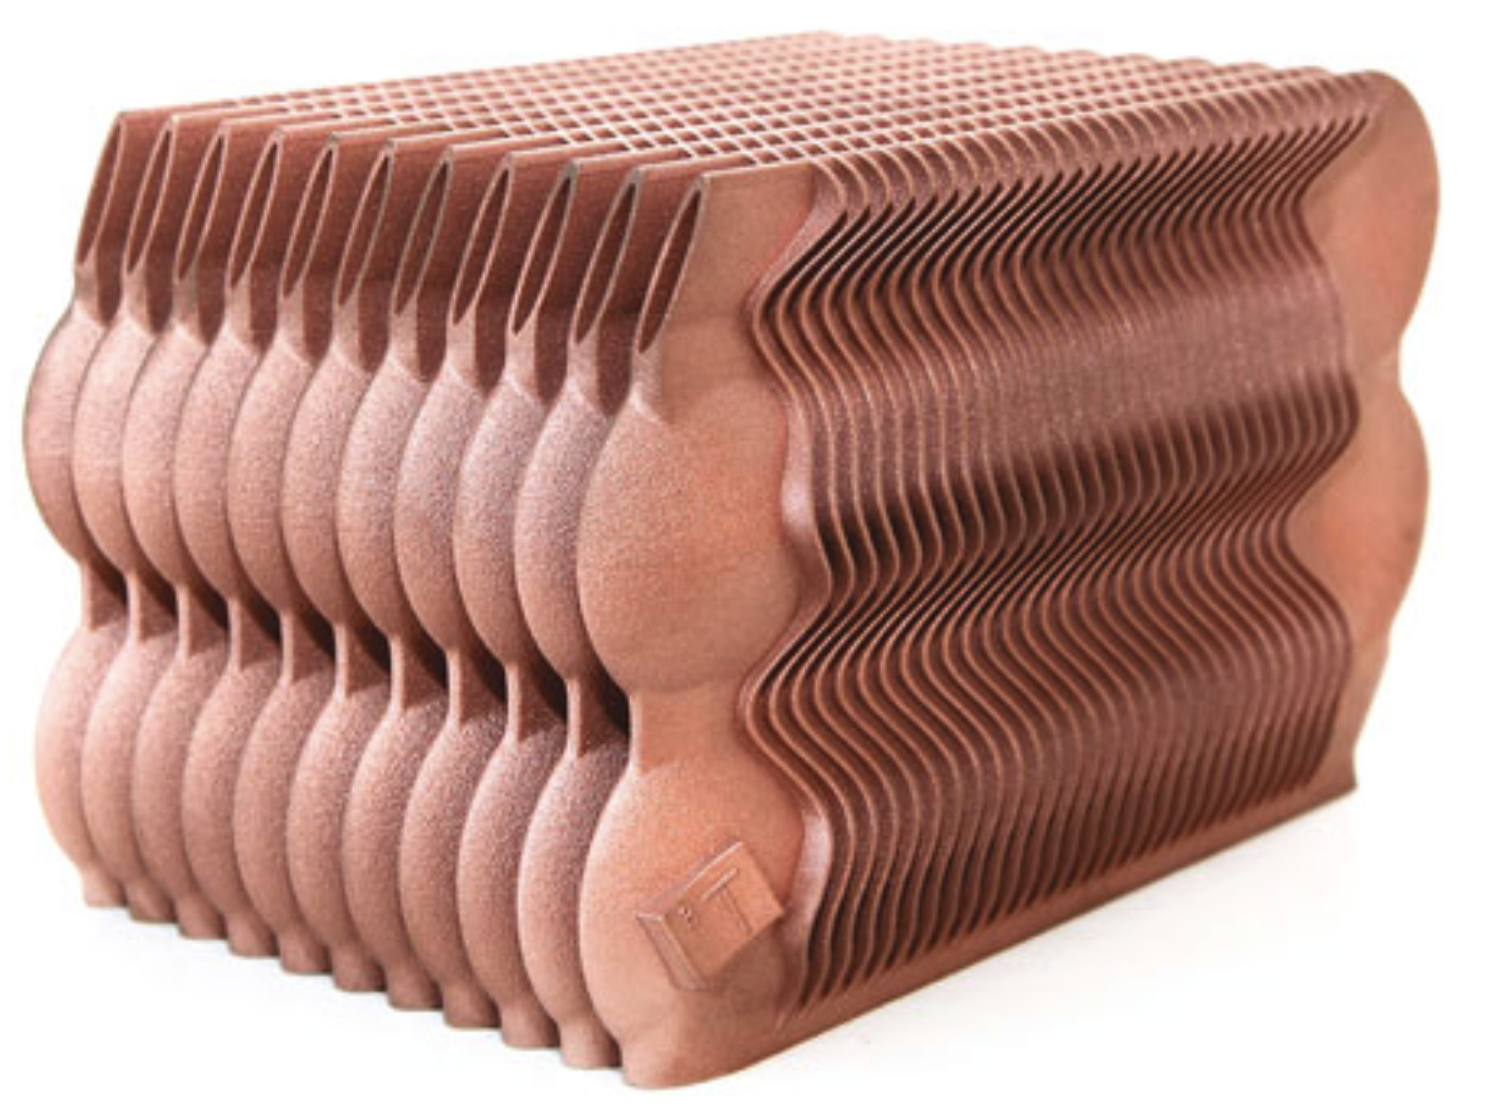
\includegraphics[scale=0.25]{Images/heatexchanger.png}
    }
    \qquad
    \subfloat[\label{fig:f1freno}]{
        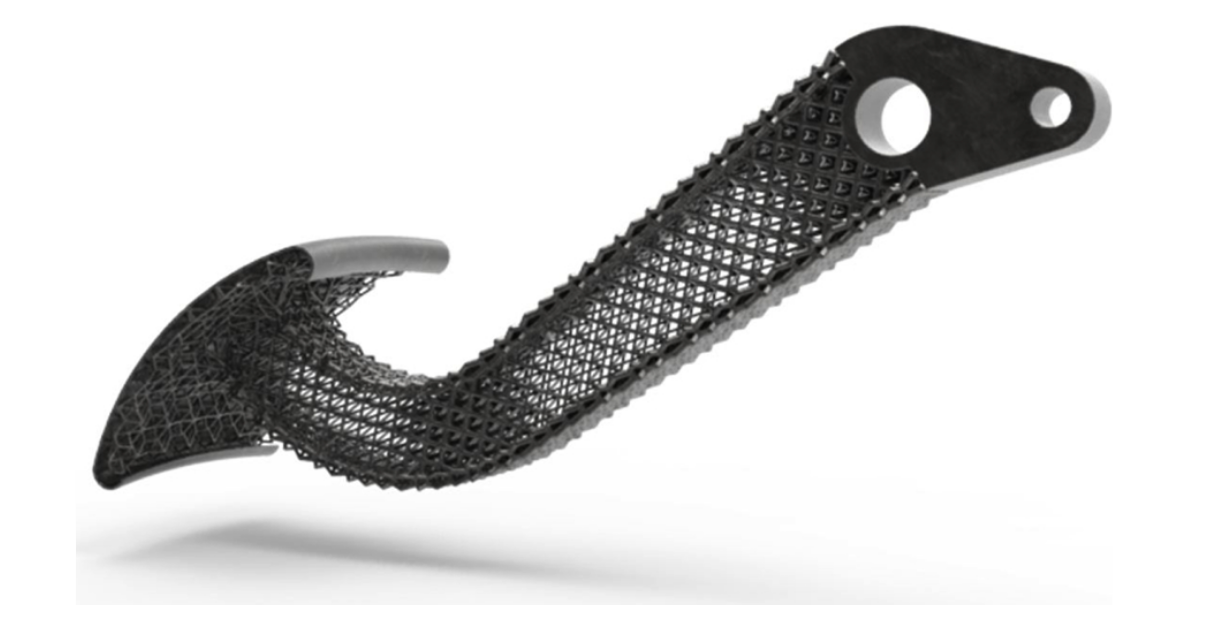
\includegraphics[scale=0.3]{Images/f1freno.png}
    }
    \caption[Lattice structure applications.]{Some lattice structure application: a complex heat exchanger (a) and brake pedal of F1 racing car (b) \cite{milewski_additive_2017, du_plessis_beautiful_2019}}.
\end{figure}

Lattice structures can be used for all these purposes, highlighting the incredible connection between nature and engineering. Lattice structures are versatile and can be effectively applied in various engineering fields to address multiple challenges. Specifically, they are commonly used in four main areas according to \citeauthor{bhate_classification_2019} (2019): 
\begin{itemize}
    \item \textbf{Structural engineering} for vibration control, strain isolation, and weight reduction purposes like in Fig. \ref{fig:f1freno};
    \item \textbf{Thermal engineering} for applications such as heat exchangers in Fig. \ref{fig:heatexchanger}, flame arresters, or heat shields;
    \item \textbf{Fluid dynamics engineering} which employs lattice structures as catalyst carriers or packaging;
    \item \textbf{Biomedical engineering}, where lattice structure can be leveraged for bone integration in prosthetic and cell growth
\end{itemize}
% <<< End of Applications of PBF Metal Additive Manufacturing
% <<< end of PBF processes


% Hot Spot Defect >>>
\chapter{Hot Spot Defects in PBF Processes}
\label{ch:hotspot}%
\input{hotspot}
% <<< end of Hot Spot Defect

% Hot Spot State of the Art >>>
\chapter{Hot Spot Detection: a State of the Art Research}
\label{ch:state_ot_the_art}%
This chapter will focus on machine learning algorithms for hot spot detection. Since I want this chapter to be entirely understandable to as many readers as possible, I will provide a brief introductory overview to elucidate the fundamental aspects in Section \ref{sec:introperritardati}. For a detailed understanding of the research strategy employed to write this state-of-art review, please refer to Appendix \ref{ap:research}. 

\section{Warm Up}
\label{sec:introperritardati}
In this section, I will explain some fundamental concepts that are essential for fully understanding of next section and also \emph{Chapter ~\ref{ch:baggingvoronoi}}. If the reader is already familiar with these concepts, they can comfortably proceed to Section \ref{sec:hotspotstateart}. 

% Machine learning>>>
\subsection{Machine Learning}
\label{subsec:ml}
In recent years, the volume of data and the speed at which data are available have increased exponentially. Thus, there is a need for new tools we can leverage in order to find valuable and actionable insights from this huge amount of data. The set of activities involved in the analysis of these large sets of data, usually with the purpose of extracting useful knowledge to support decision-making, has been referred to as machine learning \cite{vercellis_business_2009}. \emph{Machine learning} (ML) is an approach that involves the development of algorithms that enable computers to learn from and find patterns in a large amount of data. Rather than being explicitly programmed to perform a task, a machine learning system uses inference to make predictions or decisions based on input data, trying to minimize somehow the output error or a cost function. Formally, \textit{“A computer program is said to learn from experience $E$ with respect to some class of task $T$ and a performance measure $P$, if its performance at tasks in $T$, as measured by $P$, improves because of experience $E$”} \cite{zaki_data_2020, pierluca_lanzi_data_2021}. Suppose we have the experience $E$, a set of observations of a specific phenomenon, encoded as a dataset
\begin{equation}
    \label{eq:dataset}
    \mathbf{E}=\{\mathbf{x}_1, \dots, \mathbf{x}_N\} 
\end{equation}
where $\mathbf{x}_i\in \mathbb{R}^p$ is a $p$ dimensional vector, containing the realization of the $p$ features of the dataset. We have three possible scenarios:
\begin{itemize}
    \item \textbf{Supervised learning:} given the records of the dataset and respective desired outputs $t_1, t_2, \dots, t_N$, also known as labels, the algorithm learns how to produce the correct output given a new set of input;
    \item \textbf{Unsupervised learning:} given $\mathbf{E}$, the algorithm is used to exploit regularities, usually used as input for supervised learning algorithm, for explaining the observations or for classification;
    \item \textbf{Reinforcement learning:} the algorithm producing actions $a_1, a_2, \dots, a_H$ which affect the environment, and receiving rewards $r_1, r_2, \dots, r_H$, learn how to act in order to maximize rewards in the long term.
\end{itemize}
To further highlight the difference between supervised and unsupervised learning, it's important to note that unsupervised learning is also defined as "learning without a teacher" in \citeauthor{tibshirani_elements_2008} (2008). So, the main difference between supervised and unsupervised learning is the input data: in the former case, data is labeled a priori, while in the latter case is not. 
% <<< end of Machine learning

%%%%%
%%%%%

% Clustering algorithms >>>
\subsection{Clustering Algorithms}
\label{sec:clustering}
\emph{Clustering} is an unsupervised learning technique. All clustering algorithms aim to organize a collection of entities $\mathbf{E}$ into subsets or "clusters" wherein elements within a cluster are as similar as possible. In contrast, data in different groups are as dissimilar as possible. So, clustering aims to minimize the within-clusters variance while maximizing the between-clusters variance. But how do we define if two observations in $\mathbf{E}$ are similar? We have to rely on the concept of distance between two observations. There are several different definitions of distances. In general, given a space $\mathbb{R}^p$ and a set of points on this space, a distance measure $d\left(\mathbf{x}_1,\mathbf{x}_2\right)$ is a function mapping two points $\mathbf{x}_1\in\mathbb{R}^p$ and $\mathbf{x}_2\in\mathbb{R}^p$ to a real number, and satisfies these axioms:
\begin{enumerate}
    \item $d\left(\mathbf{x}_1,\mathbf{x}_2\right) \geq 0$
    \item $d\left(\mathbf{x}_1,\mathbf{x}_2\right) = d\left(\mathbf{x}_2,\mathbf{x}_1\right)$
    \item $d\left(\mathbf{x}_1,\mathbf{x}_2\right)=0 \Leftrightarrow \mathbf{x}_1 = \mathbf{x}_2$
    \item $d\left(\mathbf{x}_1,\mathbf{x}_2\right) \leq d\left(\mathbf{x}_1,\mathbf{x}_3\right) + d\left(\mathbf{x}_1,\mathbf{x}_3\right)$
\end{enumerate}
where $\mathbf{x}_3 \in \mathbb{R}^p$ is a third point in the space. Recalling that $\mathbf{x}_1=\left(x_{11}, x_{12}, \dots, x_{1p} \right)$ and $\mathbf{x}_2=\left(x_{21}, x_{22}, \dots, x_{2p} \right)$, most used distance measure:
\begin{itemize}
    \item Euclidean distance
\begin{equation}
    \label{eq:euclidean}
    d\left(\mathbf{x}_1,\mathbf{x}_2\right) = \sqrt{\sum_{i=1}^p\left(x_{1i}-x_{2i} \right)^2}
\end{equation}
\item Manhattan distance
\begin{equation}
    \label{eq:mandistance}
    d\left(\mathbf{x}_1,\mathbf{x}_2\right) = \sum_{i=1}^p\left|x_{1i}-x_{2i} \right|
\end{equation}
\item Mahalanobis distance
\begin{equation}
    \label{eq:mahadistance}
    d(\mathbf{x}_1, \mathbf{x}_2) = \sqrt{(\mathbf{x}_1 - \mathbf{x}_2)^\mathrm{T} \Sigma^{-1} (\mathbf{x}_1 - \mathbf{x}_2)}
\end{equation}
where $\Sigma^{-1}$ it's the inverted covariance matrix of the dataset.
\item Jaccard distance, used in the case of cathegorical features, once they have been encoded using one-hot encoding
\begin{equation}
    \label{eq:jaccard}
    d\left(\mathbf{x}_1, \mathbf{x}_2\right) = 1 - J\left(\mathbf{x}_1, \mathbf{x}_2\right)
\end{equation}
where 
\begin{equation}
J\left(\mathbf{x}_1, \mathbf{x}_2\right) = \frac{\left|\mathbf{x}_1 \cap \mathbf{x}_2\right|}{\left|\mathbf{x}_1 \cup \mathbf{x}_2\right|}    
\end{equation}
\end{itemize}
There are several different clustering algorithms that can be divided into two main groups, as in \citeauthor{james_introduction_2021} (2021): K-Means clustering and hierarchical clustering. In \emph{K-Means clustering}, we try to divide observation into a specified number of clusters. On the other hand, in \emph{hierarchical clustering}, we do not specify the number of clusters in advance, but we rely on the dendrogram, a tree-like visual representation of all clustering steps. Then, we can "cut" the dendrogram in order to select the most appropriate number of clusters for us. In Fig. \ref{fig:clustiteration}, there is an example of simulated data in the plane clustered into 3 clusters using the K-Means algorithm (that will be discussed later). It is important to note that hierarchical clustering algorithms are less computationally efficient than K-means algorithms and suffer from the combinatorial explosion as the number of observations to be clustered increases. Indeed, as we will also see in Section \ref{sec:hotspotstateart}, all the proposed methods exploit k-means algorithms.
% <<< End of Clustering algorithm

%%%%%
%%%%%

% K-means algorithms >>>
\subsubsection{K-Means Clustering Algorithm}
\label{sss:kmeans}
We will delve deeper into it in a dedicated section since we will use K-Means in Section \ref{sec:bvc} and in Appendix \ref{ap:Python}. Let $C_1,\dots,C_k$ denote the sets containing all the indices of the observation in respective the respective cluster. K-Means clustering is a straightforward clustering algorithm we can use for complete partitioning of a data collection of observations $E=\{\mathbf{x}_1, \dots, \mathbf{x}_n \}$, described by $p$ features, into $K$ distinct, non-overlapping clusters. This means that:
\begin{enumerate}
    \item $C_1 \cup C_2 \cup \dots \cup C_K=\{1,\dots,n\}$. So, each observation belongs to at least one of the $K$ clusters.
    \item $C_k\cap C_{k'}=0$ for all $k\neq k'$. In other words, no observation belongs to more than one cluster.
\end{enumerate}
Thus, each observation will be assigned to one cluster and one cluster only. Moreover, each cluster $C_i$ has a representative point that summarizes the cluster. That's the centroid $\bm{\mu}_i$
\begin{equation}
    \label{eq:centroid}
    \boldsymbol{\mu}_i=\frac{1}{\left|C_i\right|} \sum_{x_j \in C_i} \mathbf{x}_j
\end{equation}
K-means begins by randomly placing $\bm{\mu}_i \in \mathbb{R}^p$ for $i=1,\dots,K$ points as initial cluster centroids. This is usually achieved by generating a random value within the bounds of each dimension. 
\begin{figure}
    \centering
    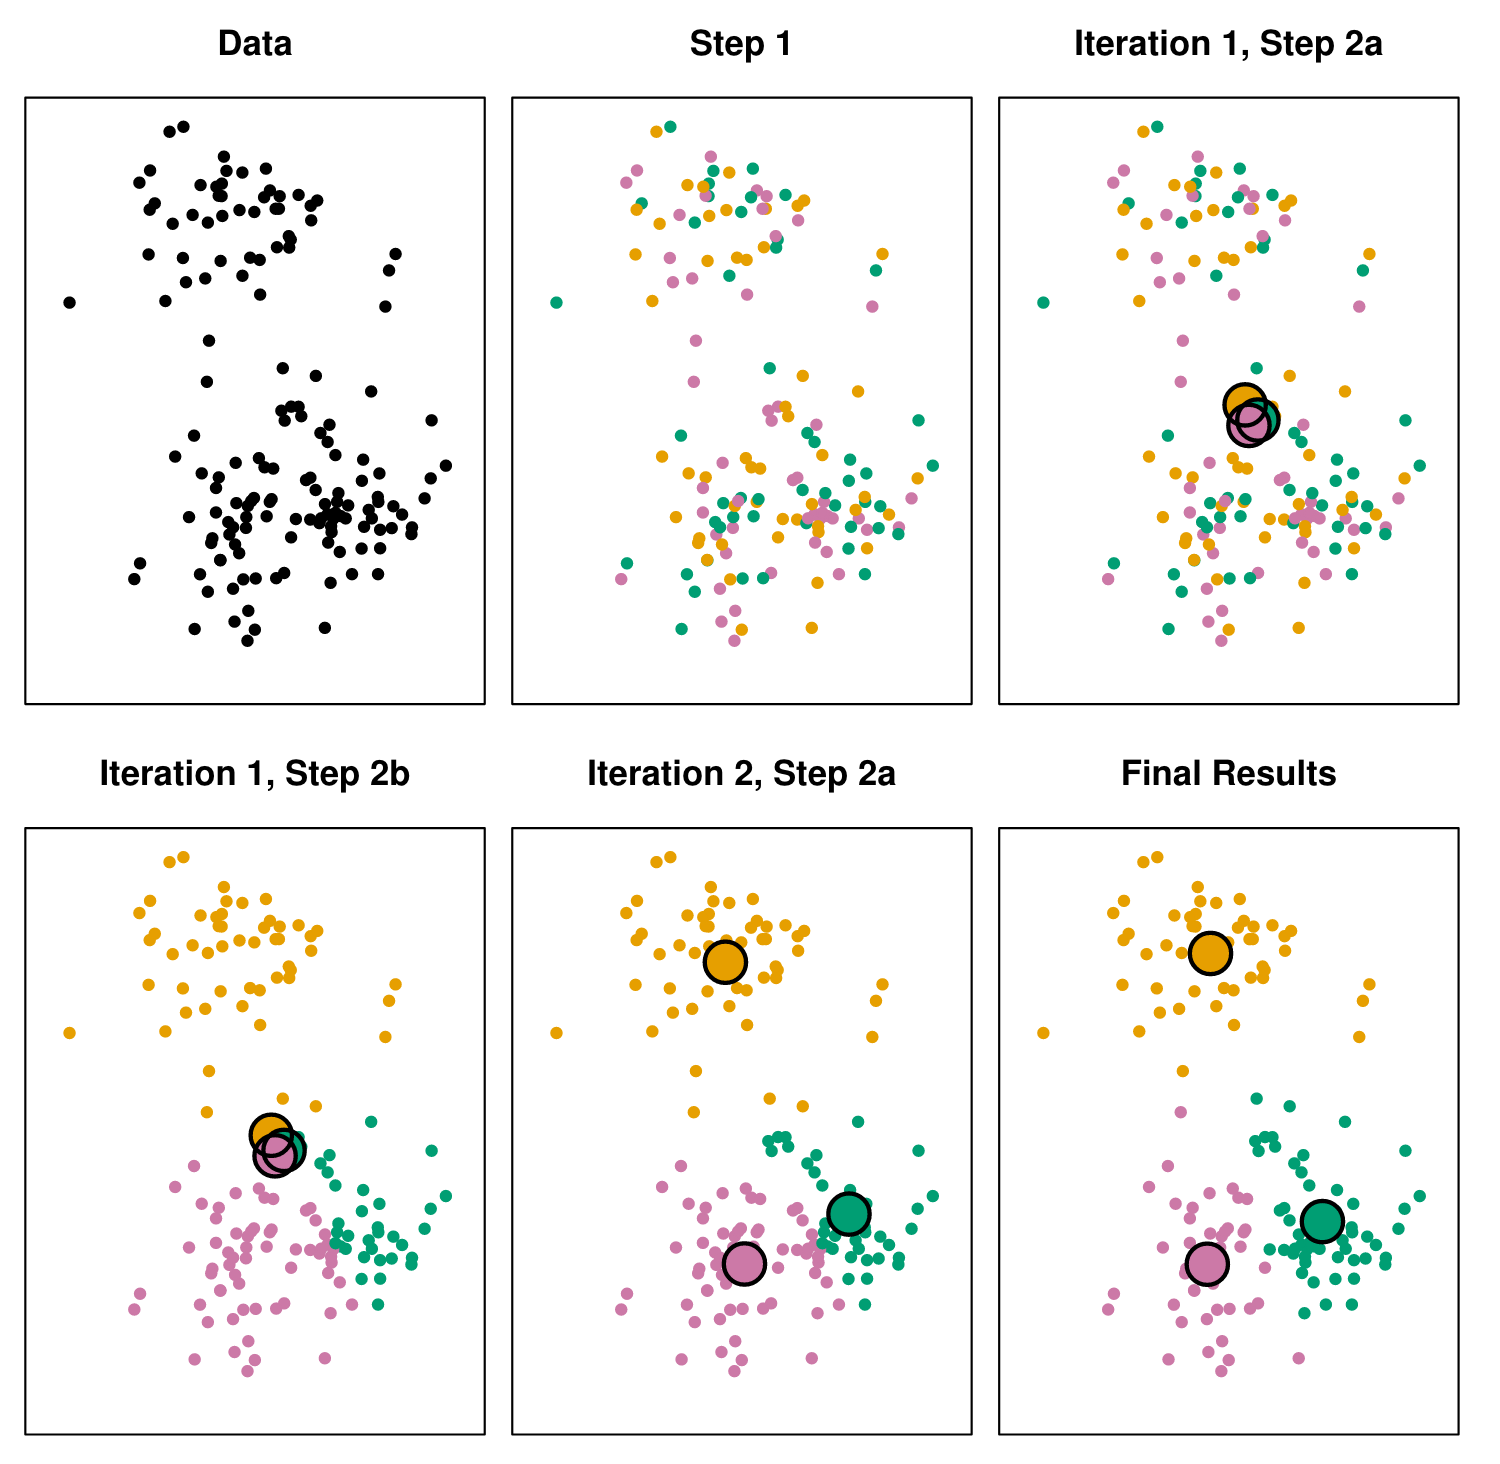
\includegraphics[width=0.6\textwidth]{Images/clustiteration.png}
    \caption[K-Means clustering iterations.]{The progress of the K-means algorithm with $K=3$ \cite{james_introduction_2021}.}
    \label{fig:clustiteration}
\end{figure}
The K-means algorithm progresses through iterative cycles involving two primary actions: (i) assigning data points to clusters and (ii) updating centroids. Given the $K$ centroids, the assignment phase allocates each data point to its nearest centroid, resulting in distinct clusters, where each cluster $C_i$ consists of points closer to its centroid $\bm{\mu}_i$ than to any other centroid. Then, in the update phase, each cluster's centroid is recalculated based on its (updated) member data points. This iterative process of assignment and updating continues until the centroids stabilize. In practical terms, K-means can be considered stable when there's no shift in centroid positions between consecutive iterations. We can adjust the tolerance parameter $\epsilon \geq 0$ for early termination of the algorithm or let the algorithm converge to the local optimum until observations no longer change cluster. In algorithm \ref{alg:kmeans}, there is the pseudo-code of the K-Means clustering algorithm.
\begin{algorithm}
\small
    \caption{K-Means Clustering}
    \label{alg:kmeans}
    \begin{algorithmic}[1]
    \STATE {$t=0$}
    \STATE {Randomly initialize $K$ centroids: $\bm{\mu}_1^t, \bm{\mu}_2^t, \dots, \bm{\mu_k^t} \in \mathbb{R}^p$}
    \REPEAT
    \STATE {$t \leftarrow t + 1$}
    \STATE {$C_i \leftarrow \empty$ for all $i=1,\dots,K$}
    \STATE {//Cluster assignment step}
    \FORALL{$\mathbf{x}_j\in D$}
    \STATE {$i^* \leftarrow \arg \min _i\left\{\left\|\mathbf{x}_j-\boldsymbol{\mu}_i^{t-1}\right\|^2\right\}$}
    \STATE {$C_{i^*} \leftarrow C_{i^*} \cup\left\{\mathbf{x}_j\right\} / / \text { Assign } \mathbf{x}_j \text { to closest centroid }$}
    \ENDFOR
    \STATE {//Centroid update Step}
    \FORALL{$i=1,\dots,K$}
    \STATE{$\boldsymbol{\mu}_i^t \leftarrow \frac{1}{\left|C_i\right|} \sum_{\mathbf{x}_j \in C_i} \mathbf{x}_j$}
    \ENDFOR
    \UNTIL{$\sum_{i=1}^k\left\|\boldsymbol{\mu}_i^t-\boldsymbol{\mu}_i^{t-1}\right\|^2 \leq \epsilon$}
    \end{algorithmic}
\end{algorithm} 
Since the initial guess of the centroids can lead to different labeling of the same observation, the K-means algorithm is typically run several times. In bagging clustering, we run the algorithm multiple times, and the final label is defined by majority voting across the different intermediate clusterizations.
% <<< End of K-means clustering algorithmclassification


% Principal component analysis >>>
\subsection{Principal Component Analysis}
\label{subsec:PCA}
Another unsupervised machine learning technique is the principal component analysis (PCA). This method leverages the information patterns within the dataset to reduce the problem's dimensionality. Principal components (PC) of a set of data in $\mathbb{R}^p$ provide a sequence of best linear approximation to that data of all ranks $q\le p$ \cite{james_introduction_2021, tibshirani_elements_2008}. \emph{Principal component analysis} refers to the process by which principal components are computed. Suppose we have a dataset that represents experience $\mathbf{E}$ of a certain phenomenon, of unlabeled data and each realization $\mathbf{x}_j \in \mathbb{R}^p$ for all $j=1,\dots,n$. Thus, $\mathbf{E} \in \mathbb{R}^{n\times p}$. The first principal component of a set of features $\mathbf{X}_1, \mathbf{X}_2, \dots, \mathbf{X}_p$ is the normalized linear combination of the features
\begin{equation}
    \label{eq:firstPC}
    Z_1=\phi_{11} \mathbf{X}_1+\phi_{21} \mathbf{X}_2+\cdots+\phi_{p1} \mathbf{X}_p
\end{equation}
By normalized, we mean that $\sum_{j=1}^p\phi_{j1}^2=1$. The elements $\phi_{11},\dots,\phi_{p1}$ are the loadings of the first principal component. But how can we find PCs? Suppose we want to find a linear model representing the $i$-th observation. We are trying to find a linear combination such as:
\begin{equation}
    \label{eq:pcaf}
    f(\lambda)=\bm{\mu}+\mathbf{V}_q\bm{\lambda}
\end{equation}
where $\bm{\mu}\in \mathbb{R}^p$ is a location vector, $\mathbf{V}_q$ is a $p\times q$ matrix with $q$ orthogonal unit vectors as columns, and $\bm{\lambda \in \mathbb{R}^q}$ is a vector of $q$ parameters. So, we can fit the model to the data by minimizing the sum of least squared errors:
\begin{equation}
    \label{eq:SSE}
    \min _{\bm{\mu},\left\{\lambda_i\right\}, \mathbf{V}_q} \sum_{j=1}^N\left\|\mathbf{x}_j-\bm{\mu}-\mathbf{V}_q \lambda_j\right\|^2
\end{equation}
We can partially optimize for $\bm{\mu}$ and the $\lambda_j$ to obtain
\begin{equation}
    \hat{\bm{\mu}} = \left(E\left(\mathbf{X}_1\right), E\left(\mathbf{X}_1\right), \dots, E\left(\mathbf{X}_p\right)\right)
\end{equation}
\begin{equation}
    \hat{\lambda}_j = \mathbf{V}_q^{T}(\mathbf{x}_j-\hat{\bm{\mu}})
\end{equation}
This leads to 
\begin{equation}
\label{eq:diocaro}
    \min _{\mathbf{V}_q} \sum_{i=1}^N\left\|\left(\mathbf{x}_j-\hat{\bm{\mu}}\right)-\mathbf{V}_q \mathbf{V}_q^T\left(\mathbf{x}_j-\hat{\bm{\mu}}\right)\right\|^2
\end{equation}
The $q \times q$ matrix $\mathbf{H}_q=\mathbf{V}_q\mathbf{V}_q^T$ is a projection matrix and maps each point $\mathbf{x}_j$ onto it's rank~-~$q$ reconstruction $\mathbf{H}_qx_j$, the orthogonal projection of $x_j$ onto the subspace spanned by the columns of $\mathbf{V}_q$. The solution can be expressed as follows. Stacked the centered observations into rows of an $N\times p$ matrix $\mathbf{E}$, we can construct the singular value decomposition
\begin{equation}
    \label{eq:SVD}
    \mathbf{E}=\mathbf{U}\bm{\Sigma}\mathbf{V}^T
\end{equation}
where $\mathbf{U}$ and $\mathbf{V}$ are unitary matrices and $\bm{\Sigma}$ is a $p \times p$ diagonal matrix, such that $\sigma_{11}\ge \sigma_{22} \ge \dots \ge \sigma_{pp}\ge 0$. This means that $\mathbf{u}_1$ and $\mathbf{v}_1$ correspond to $\sigma_{11}$ and are somehow more important with respect to $\mathbf{u}_2$ and $\mathbf{v}_2$ which are associated to $\sigma_{22}$ in explaining the information in $\mathbf{E}$ and so on and so forth. The columns of $\mathbf{U}$ are the basis vector of the new space, and the columns of $\mathbf{U}\mathbf{D}$ are the principal components. The $\sigma_{ii}$ are also called singular values and are the variance the $i$-th PC explains. Lastly, $\mathbf{v}_i=(\phi_{11} \dots \phi_{p1})$ re the loading vectors of such $i$-th PC.  For each rank $q$, the solution $\mathbf{V}_q$ to Eq. \ref{eq:diocaro}, consist of the first $q$ columns of $\mathbf{V}$. A good method to determine the number $q$ of principal components (PC) is to rely on the scree plot of explained variance. Indeed, the variance explained by each additional PC follows the law of diminishing returns. Therefore, we can decide how many PCs when we observe a significant knee in the graph.

\subsubsection{PCA for Spatial and Temporal Data}
We can also apply PCA to spatial, temporal, or spatiotemporal data. We can also use PCA with images or image streams (videos). Indeed, we can see images as two-dimensional arrays and videos as three-dimensional arrays, in which, along the third dimension, we have time evolution. The most common approach is the \emph{S-mode} PCA, where frame pixels are treated as variables (columns of the dataset) and frames as observations (rows of the dataset). In this way, each frame is unfolded and interpreted as a single dataset entry. By doing so, a video of $J$ frames, each of dimension $M\times N$ can be see as a dataset $\mathbf{X}\in\mathbb{R}^{J\times P}$ where $P=M\times N$. The S-mode captures the correlation of pixels in space to determine how outlying each frame is with respect to the set of considered images. However, the phenomenon's evolution from frame to frame can cause local defects to be hidden. The S-mode PCA approach lacks any spatial localization capability \cite{colosimo_spatially_2018}. Further approaches are the so-called Tensor-based PCA. Multi-linear PCA and the tensor rank-one decomposition are some examples. These methods allow us to pay attention to the temporal effect as in S-mode PCA by not unfolding the image but applying a higher-order PCA. In this sense, the tensor projected onto the low-dimensional space can capture most of the variability of the data, including both spatial and temporal contributions. In the field of quality control, we can use Hotelling's T2, which associates each frame with a synthetic value and makes it possible to identify a shift from the nominal process conditions. Formally, it finds a multi-linear transformation that maps the original tensor space $\mathbb{R}^{M \times N \times J}$ into a tensor subspace $\mathbb{R}^{P_1 \times P_2 \times J}$ with $P_1<M$ and $P_2<N$, where $M$ and $N$ are the dimensions of the video frames. $P_1$ and $P_2$ are the number of PCs retained to capture a given percentage of data variability along the "first mode" (size $M$ ) and "second mode" (size $N$ ) of the original. Lastly, there is also the \emph{T-mode} PCA. This approach interprets the video frames as columns and the pixels as dataset entries. This method captures the temporal auto-correlation of pixel intensity in consecutive frames. In this way, the array $\mathbf{U}\in \mathbb{R}^{M\times N \times J}$ will become the dataset $\mathbf{X}\in \mathbb{R}^{PxJ}$ where $P=M\times N$. The projections of the original image data onto the first retained PCs belong to the image space, and hence, they let a spatial localization of anomalous regions. In this case, however, the spatial S-mode information is completely lost, given that no real distance between pixels is considered. In \citeauthor{colosimo_spatially_2018}, the authors presented an ST-PCA. We will see it in Section \ref{sec:hotspotstateart} as a method to detect HS.

\subsubsection{Handwritten Digits}
This example is  from \citeauthor{tibshirani_elements_2008} (2008).
The authors applied PCA to a dataset containing handwritten digits. Let's consider its application on the digit "3". Authors experimented on a set of 130 3s randomly sampled from a total of 658 total observations. Each image is a \numproduct{16 x 16} gray-scale image. We can see considerable variation in writing styles, character thickness, and orientation (Fig. \ref{fig:3s}). We can unfold images and treat each of them as vectors $\textbf{x}_j \in \mathbb{R}^{256}$, and we can use PCA on the dataset $\mathbf{E}$. In this sense, we are applying an T-mode PCA applied not to the frames of a video but to several images. This technique is also called vectorized PCA (VPCA) because it involves the vectorization operation, also known as unfolding, to transform two-dimensional objects into column vectors. In this way, the projection onto the low-dimensional space will be capable of capturing the most significant spatial variability between the different scripts.
\begin{figure}
    \centering
    \subfloat[\label{fig:3s}]{
        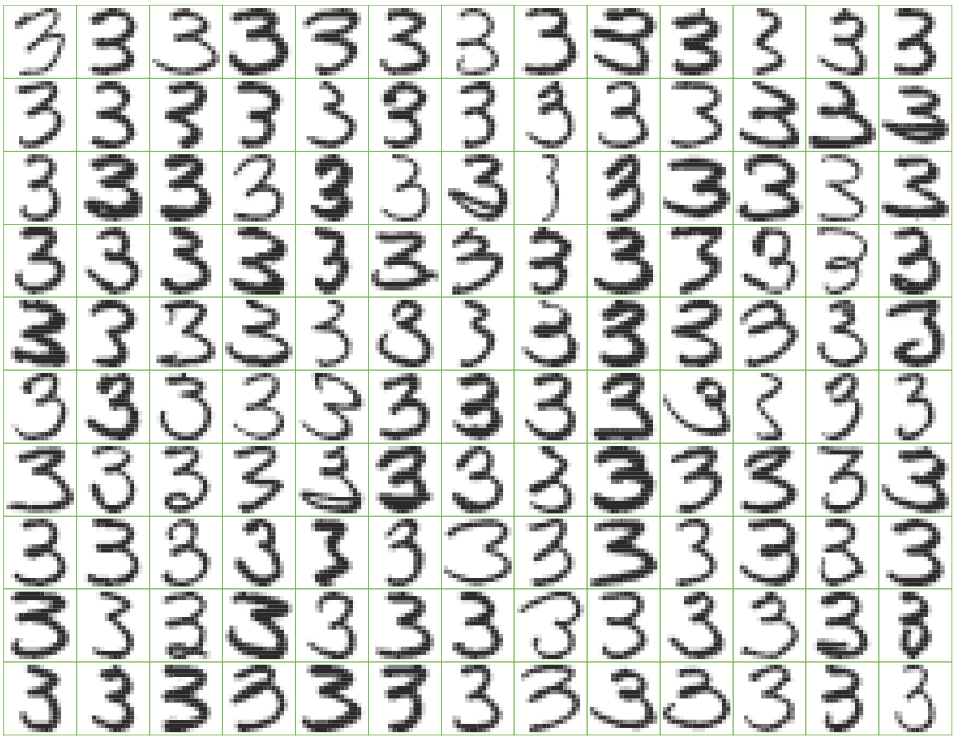
\includegraphics[width = 0.45\textwidth]{Images/1303.png}
    }
    \quad
    \subfloat[\label{fig:principal3}]{
        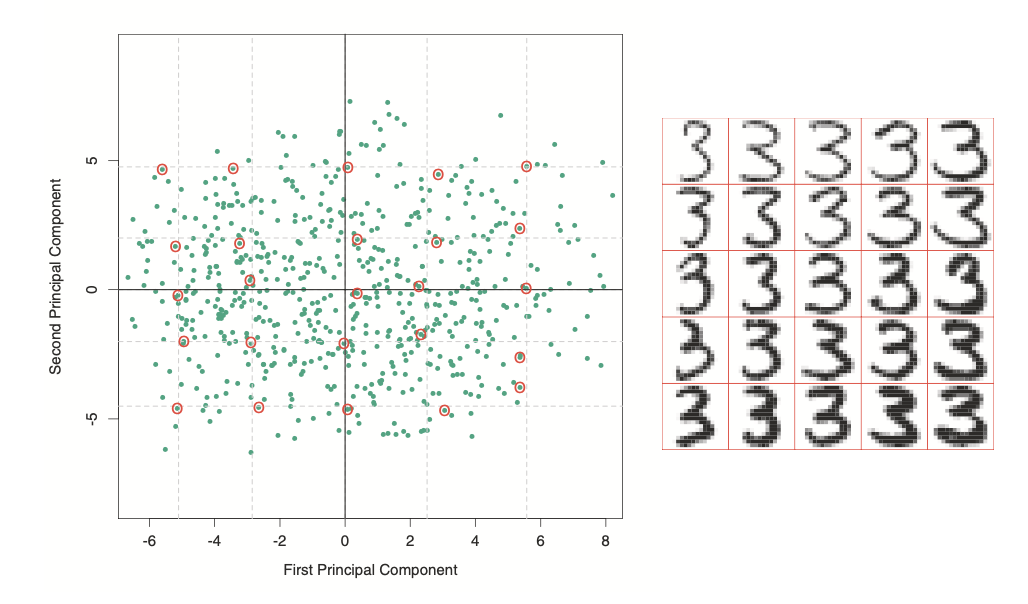
\includegraphics[width = 0.45\textwidth]{Images/pc3.png}
    }
    \caption[Example of PCA of images.]{Example of PCA applaied to images dataset: the random sample of handwritten 3s (a) and the scatterplot of the first two principal components (b) with a superimposed grid in which images match red circles on the scatterplot\cite{tibshirani_elements_2008}.}
\end{figure}
From Fig. \ref{fig:principal3}, we can see that the first PC mainly accounts for the length of the lower tail of the three, while the second PC accounts for character thickness. Then, we can reshape every PC in a matrix and interpret them as images. These images will be the base for the new vectorial space. Using just 50 PCs, we can explain 90\% of the variance of all the 3s, while with 12 PCs, we can account for 63\% of the total variance.


% <<< End of Principal component analysis


%%%%%
%%%%%


% Deep Learning, ANN and CNN >>>
\subsection{Artificial Neural Network and Deep Learnig}
\label{subsec:deepl}
In 1956, there was a summer research project on artificial intelligence at Dartmouth University. A team of professors and an expert from IBM Corporation began to think about the possibility of creating virtual neural networks. These networks would learn and enhance the purpose for which they were designed through a self-improvement process, and they could be based on the mathematical model of the human brain \cite{mccarthy_proposal_1955}. Indeed, the human brain model is especially well-suited for computational purposes. The human brain possesses a massive amount of computing units: the neurons. Approximately \num{e11} neurons in an adult human brain form about 7,000 synaptic connections with other neurons, amounting to nearly \num{e15} total synapses. Moreover, the computational model of the brain is distributed among simple nonlinear units, redundant and fault-tolerant, and capable of performing calculations in parallel \cite{matteo_matteucci_perceptrons_2021}. The mathematical virtual model of a single neuron is called a perceptron, the unitary computational unit of artificial neural networks (ANN). Just like in human neurons, the perceptron has dendrites that "collect" the charge from synapses, and once a certain threshold is exceeded, the accumulated charge is released and sent to other perceptrons. The portion of the schema in Fig. \ref{fig:perceptron} enclosed in the dashed line is called the activation function and is responsible for releasing the perceptron's accumulated charge. There are various activation functions, with some of the most common ones can be seen in Fig. \ref{fig:actfunc}.
\begin{figure}
    \centering
    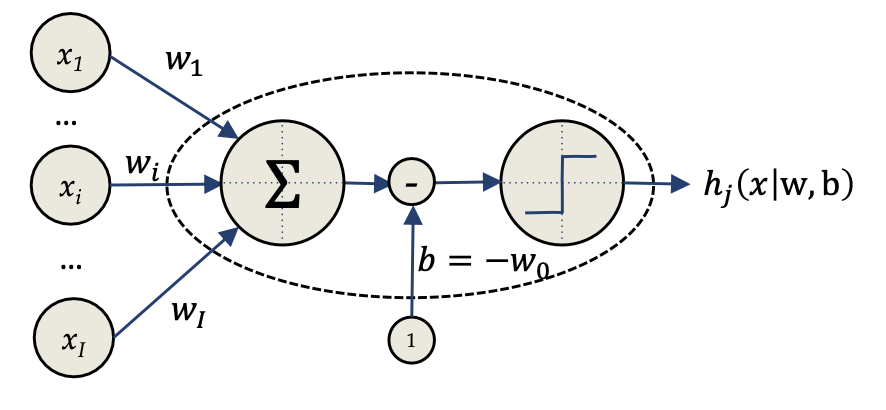
\includegraphics[width=0.6\textwidth]{Images/neurone.png}
    \caption[Perceptron schema]{Perceptron schema \cite{matteo_matteucci_perceptrons_2021}.}
    \label{fig:perceptron}
\end{figure}
Perceptrons can be combined to form networks with a layered architecture. Indeed, every neural network will have an input layer, an output layer, and a varying number of intermediate layers, known as hidden layers. Deep learning is a subfield of artificial intelligence (AI) and machine learning that involves training artificial neural networks on vast amounts of data to perform classification or regression tasks. ANNs can learn from experience $\mathbf{E}$ and understand complex patterns in data. Deep feedforward networks, also called simply feedforward neural networks or multilayer perceptrons (MLPs), are used to approximate some function $f^*$. Let's take as an example a classifier. Given an unknown function $\Lambda_0:E \rightarrow \{1,\dots,L\}$ where $\{1,\dots,L\}$ are label classes, the $f^*$ is the best approximation of the function $\Lambda_0$, defining a mapping $\mathbf{y}=f^*\left(\mathbf{x}, \bm{\theta} \right)$. The ANN learns the value of parameters $\bm{\theta}$ from $\mathbf{E}$, resulting in the best function approximation. These models are called feedforward because information flows through forward all in the network. To understand how neural networks learn from experience $\mathbf{E}$ using the chain rule and the back-propagation mechanism, readers are referred to \citeauthor{goodfellow_deep_2016} (2016).
\begin{figure}
    \centering
    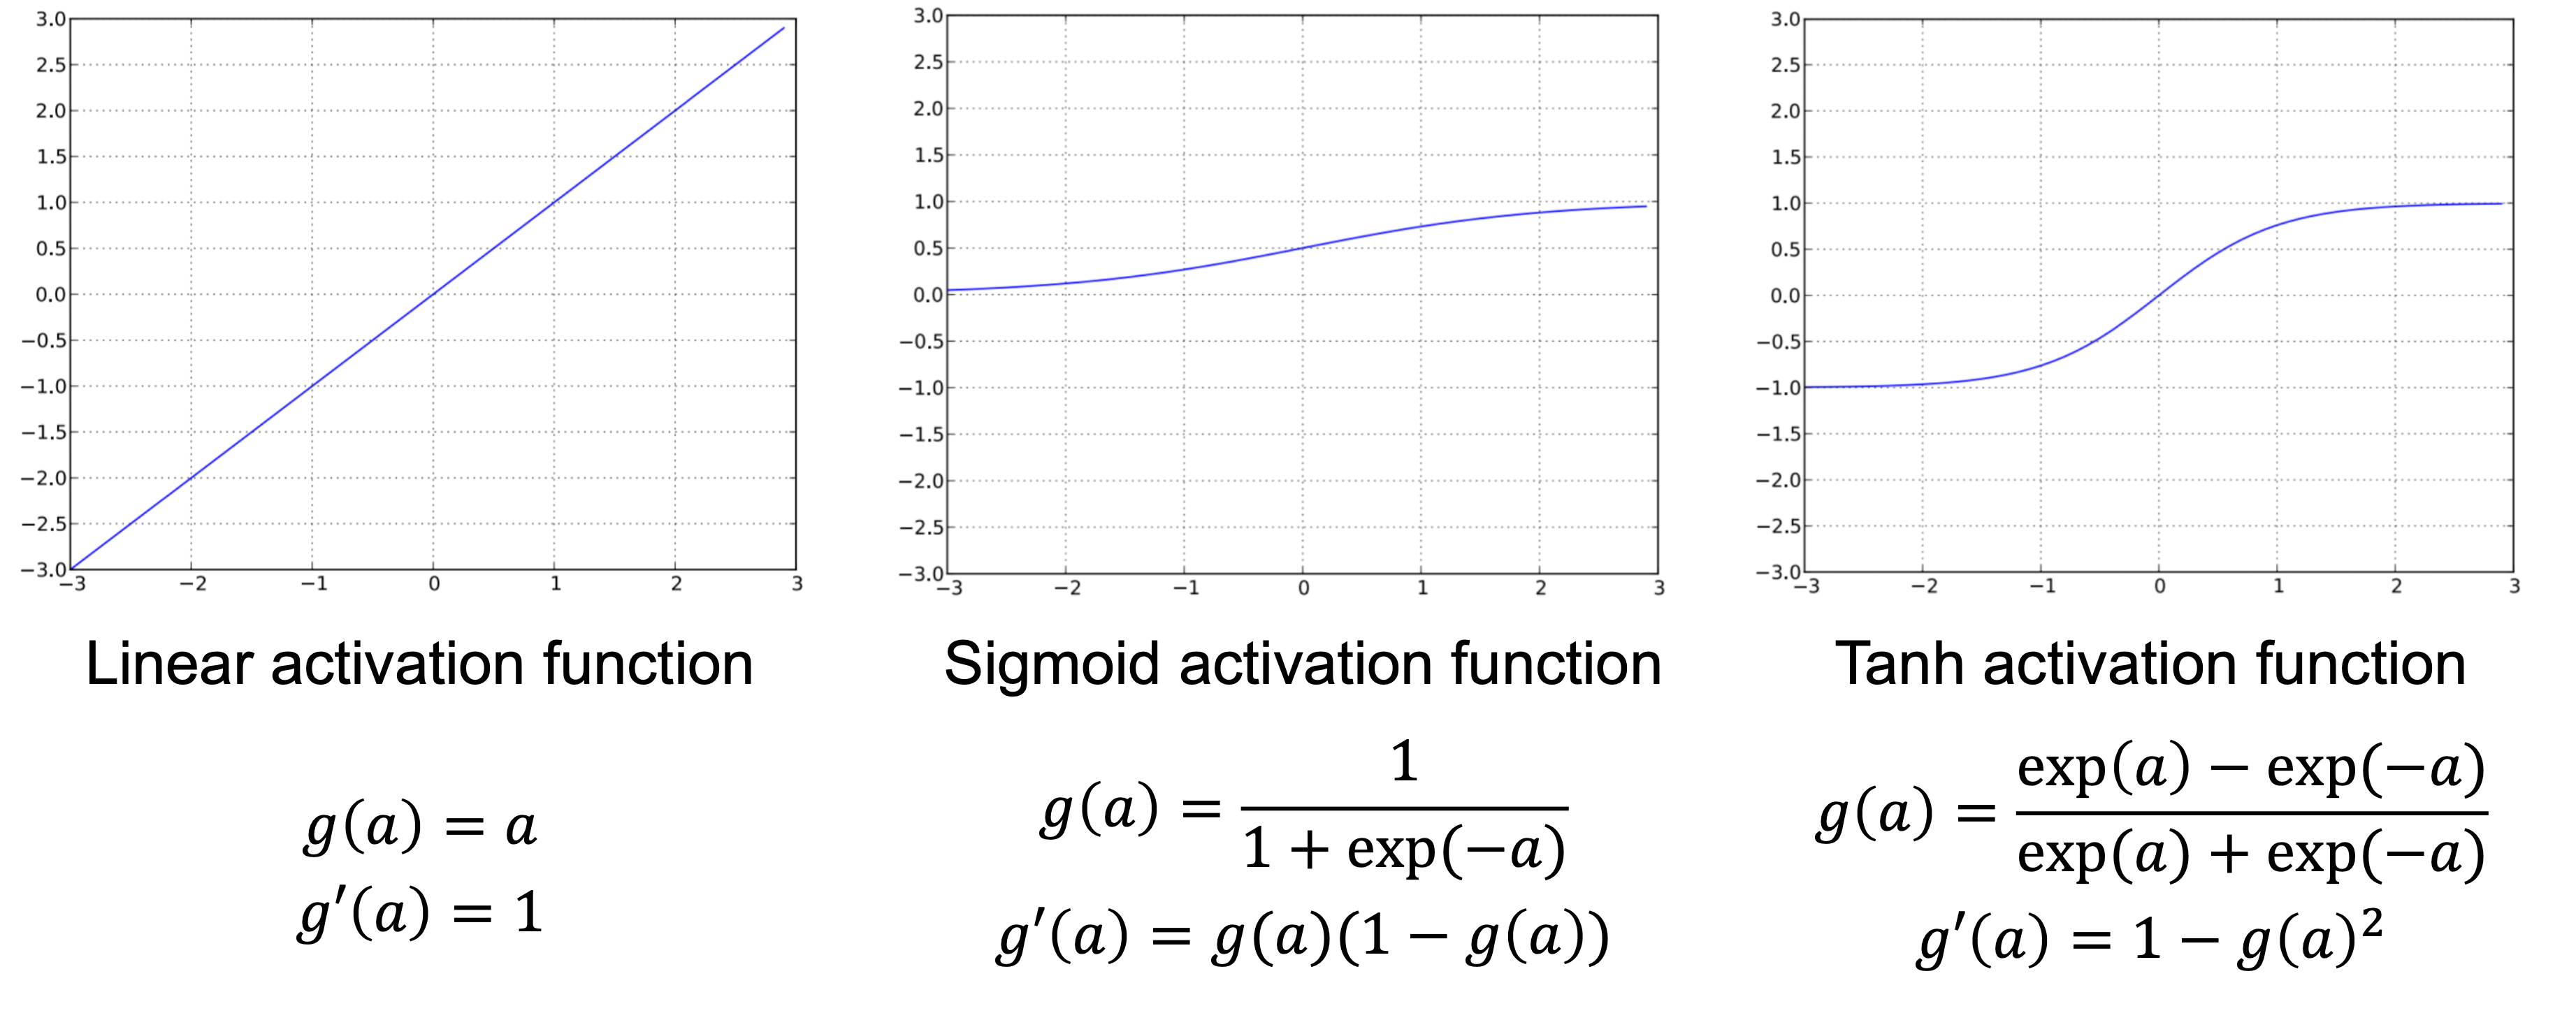
\includegraphics[width=0.8\textwidth]{Images/activationfunction.png}
    \caption[Activation functions.]{Some examples of activation functions with relatives analytical forms \cite{matteo_matteucci_perceptrons_2021}.}
    \label{fig:actfunc}
\end{figure}
Let's examine examples of how networks can address classic machine learning problems such as regression and classification. A best practice is to use tanh or sigmoid as hidden layers activation functions. Indeed, the main difference is the activation function of the output layer: 
\begin{itemize}
    \item \textbf{Regression:} since the output of a regression problem spans all $\mathbb{R}$, the activation function of the output layer will be a linear activation function;
    \item \textbf{Binary Classification:} in binary classification, the output domain is $\Omega=\{0, 1\}$. Thus, the necessary activation function for the output layer is the sigmoid activation function. The value of the function can be interpreted as class posterior probability;
    \item \textbf{Multi-class Classification:} when dealing with multiple classes ($K$), we need to use as many neurons as classes, and each output neuron will use a softmax unit. The unique feature of this activation function is that the sum of the outputs from the $K$ output neurons is equal to 1. Thus, the $k$-th output can be viewed as the probability that the input belongs to the $k$-th class.
\end{itemize}
Another typical application of neural networks is as classification algorithms for images in computer vision. However, images cannot be used directly as input since they carry too much information. We need some intermediate steps to extract useful information and reduce the problem's dimensionality by computing a feature array that summarizes the initial image's information \cite{giacomo_boracchi_convolutional_2021}. The feature array for the input layer of the classification algorithm will have a dimension of $d\ll r_1 \times c_1$ where $r_1$ and $c_1$ are the rows and the columns of the matrix representation of the image. Recall that an image can be represented as a three-dimensional matrix: the first two dimensions are pixel indexes, and the third identifies the pixel's color based on the color profile used. Take, for instance, the image in figure \ref{fig:cazzle}. The image has a width of 472 pixels a height of 376 pixels, and uses an RGB color profile. This means that three values are needed to identify the color of each pixel uniquely: the first for red, the second for green, and the third for blue. This means that we would require \numproduct{472 x 376 x 3} input neurons, one for each value of each color of each pixel of the image (more than 500,000 neurons). Feature extraction algorithms can be categorized as hand-crafted or data-driven features. With hand-crafted algorithms, we can leverage prior knowledge of the phenomenon, and features are interpretable, allowing us to exploit them even with limited data. However, this approach demands significantly more time and design/programming efforts. Moreover, it is very domain-specific and isn't so much "portable". On the other hand, data-driven feature extraction algorithms are less interpretable but offer a more robust mathematical foundation. Convolutional Neural Networks (CNNs) are neural networks that can be used for data-driven feature extraction. Given the matrix representation of the image discussed earlier, while in ANN, we talked about layers, in CNNs, we will have volumes. As the depth of such volumes increases, the height and width of the volume decreases. CNNs enable us to perform some fundamental operations essential for accurate feature extraction.
\paragraph{Convolution.} Convolutional layers "mix" all the input components. Convolution is an operation that allows us to combine all the input values from a specific region into a linear combination. Specifically, the convolution is described by the following equation:
\begin{equation}
    \label{eq:convolution}
    y_j=\sum_iw_{ij}x_i+b_j
\end{equation}
The linear combination operation is also referred to as filtering, and the parameters of this combination are called filters. The same filter is used as a sliding window through the whole spatial extent of the input images. In Fig. \ref{fig:convmatrice}, a typical convolution operation is graphically represented.
\begin{figure}
    \centering
    \subfloat[\label{fig:cazzle}]{
    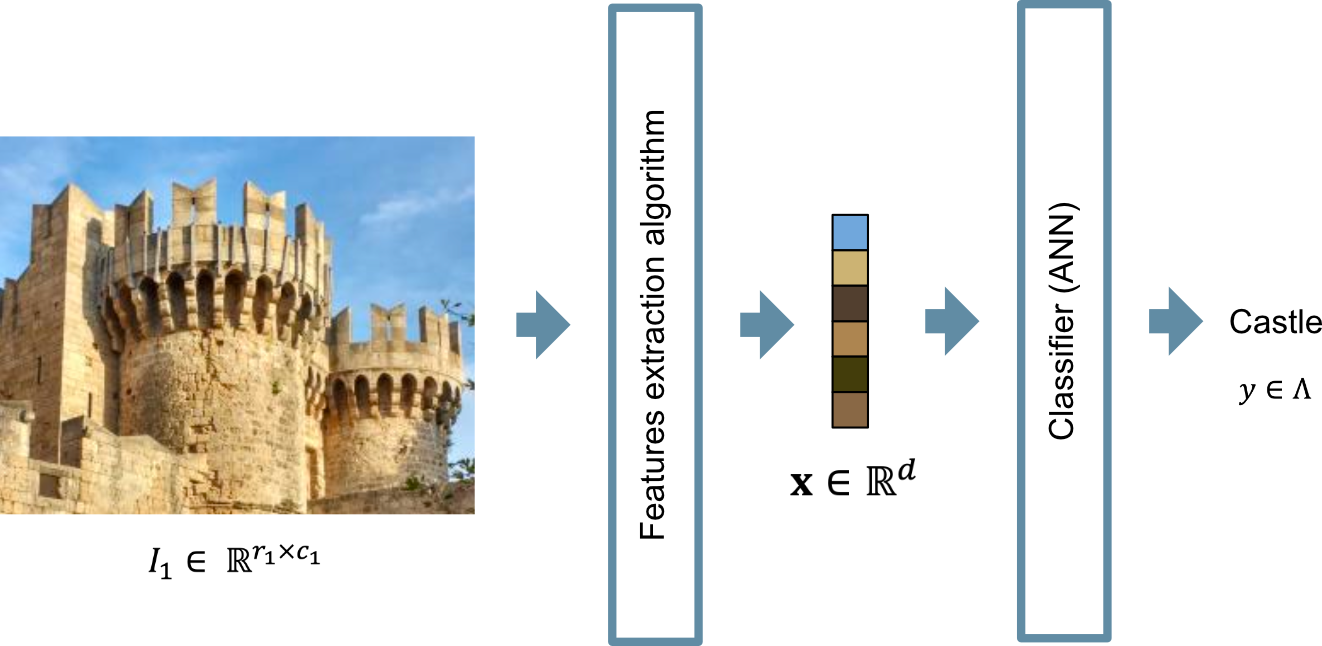
\includegraphics[width=0.7\textwidth]{Images/featureextraction.png}
    }
    \qquad
    \subfloat[\label{fig:convmatrice}]{
    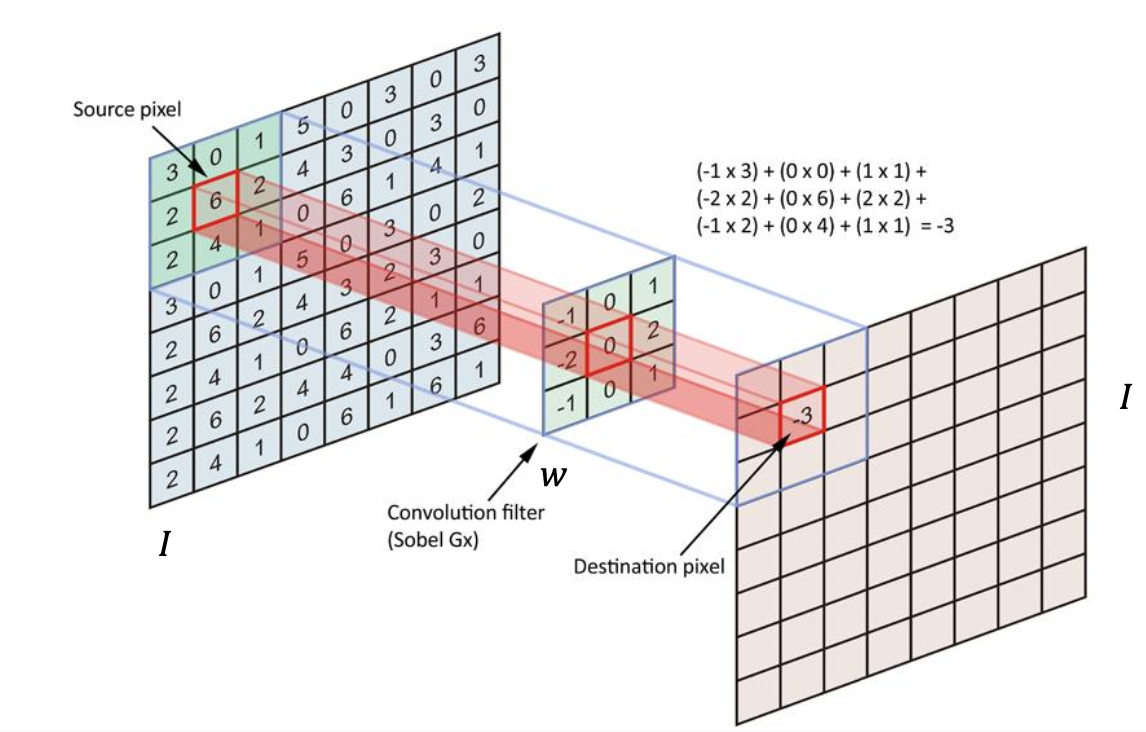
\includegraphics[width=0.5\textwidth]{Images/convolution.png}}
    \caption[Convolution operation.]{Feature extraction operation (a) adapted from \cite{giacomo_boracchi_convolutional_2021}, and convolution operation graphically represented (b)\cite{giacomo_boracchi_convolutional_2021}.}
\end{figure}
In practice, the convolution operation can be viewed as a two-dimensional window that slides across the entire image, producing an output that is a linear combination of the matrix values and their corresponding values.
\paragraph{Pooling layers.} Pooling layers reduce the spatial size of the input volume. Using the logic of a sliding window that traverses the image, a specific function is applied, often the maximum, to spatially resize the input.
\begin{figure}
    \centering
    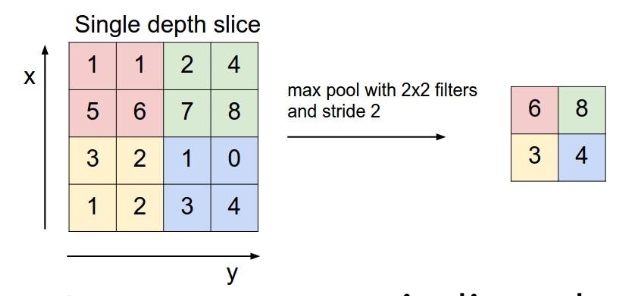
\includegraphics[width=0.5\textwidth]{Images/pooling.png}
    \caption[Pooling layer.]{Example of pooling layer that performs a max operation \cite{giacomo_boracchi_convolutional_2021}.}
    \label{fig:poolingmax}
\end{figure}
The stride parameter specifies how many elements the window shifts at once. In the figure, the window will move by two pixels simultaneously on the y-axis.
\paragraph{Activation layers.} Activation layers are used to introduce non-linearities in the network; otherwise, CNN might be equivalent to a simple linear classifier. In practice, they are layers of neurons characterized by activation functions that introduce non-linearity into the levels, just as in ANNs. We have yet to discuss two commonly used functions in these layers: the RELU (rectified linear units) and LEAKY RELU activation. The former is described as
\begin{equation}
    \label{eq:RELU}
    T(x)=\left\{\begin{array}{rr}
    x, & \text { if } x \geq 0 \\
    0, & \text { if } x<0
\end{array}\right.
\end{equation}
Whereas LEAKY RELU is similar to RELU but incorporates a slight slope for negative values, preventing neurons from dying off and becoming unresponsive after several layers. For a deeper understanding of this topic, one can refer to the vanishing gradient problem as discussed by Goodfellow.
\begin{equation}
    \label{eq:LEAKYRELU}
    T(x)=\left\{\begin{array}{rr}
    x, & \text { if } x \geq 0 \\
    k\cdot x, & \text { if } x<0
\end{array}\right.
\end{equation}
where $k$ is usually in the order of $10^{-2}$.
The convolution output will be a dense feature layer, which implies that this layer can serve as input for an ANN, which will have as many output neurons as classes in the original domain. Fig. \ref{fig:typicalcnn} shows an example of how a general CNN works.
\begin{figure}
    \centering
    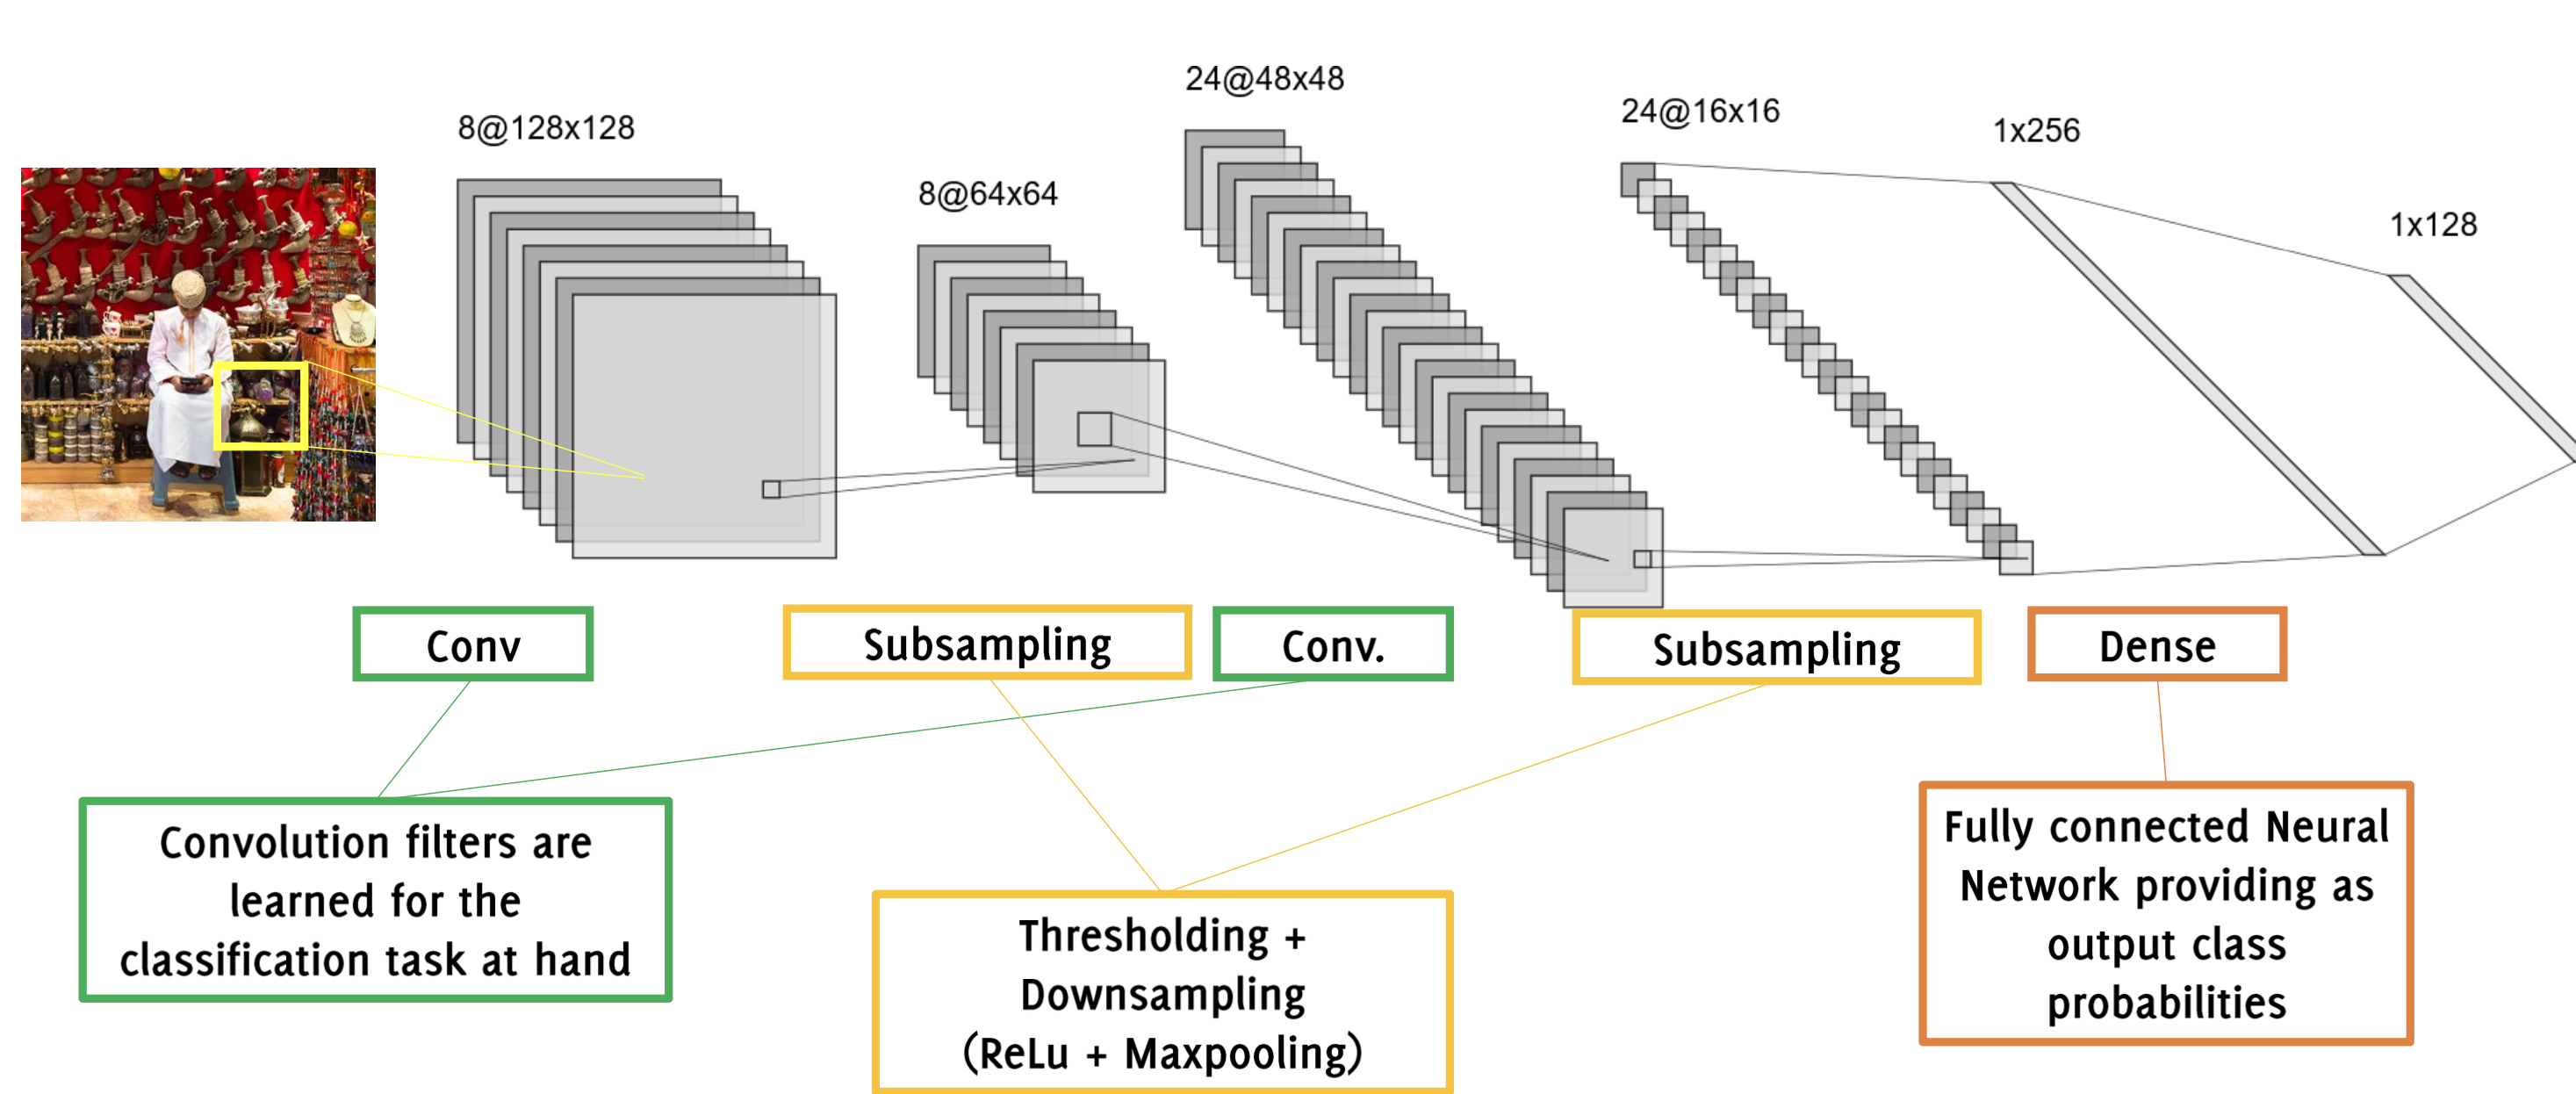
\includegraphics[width=0.8\textwidth]{Images/CNNtypical.png}
    \caption[CNN general structure.]{Graphical representation of a tipical CNN used for image classification \cite{giacomo_boracchi_convolutional_2021}.}
    \label{fig:typicalcnn}
\end{figure}
% End of Deep learning, ANN and CNN


% Deep Belief Network >>>
\subsection{Deep Belief Network}
\label{subsec:dbn}

\begin{figure}
    \centering
    \subfloat[\label{fig:l1}]{
    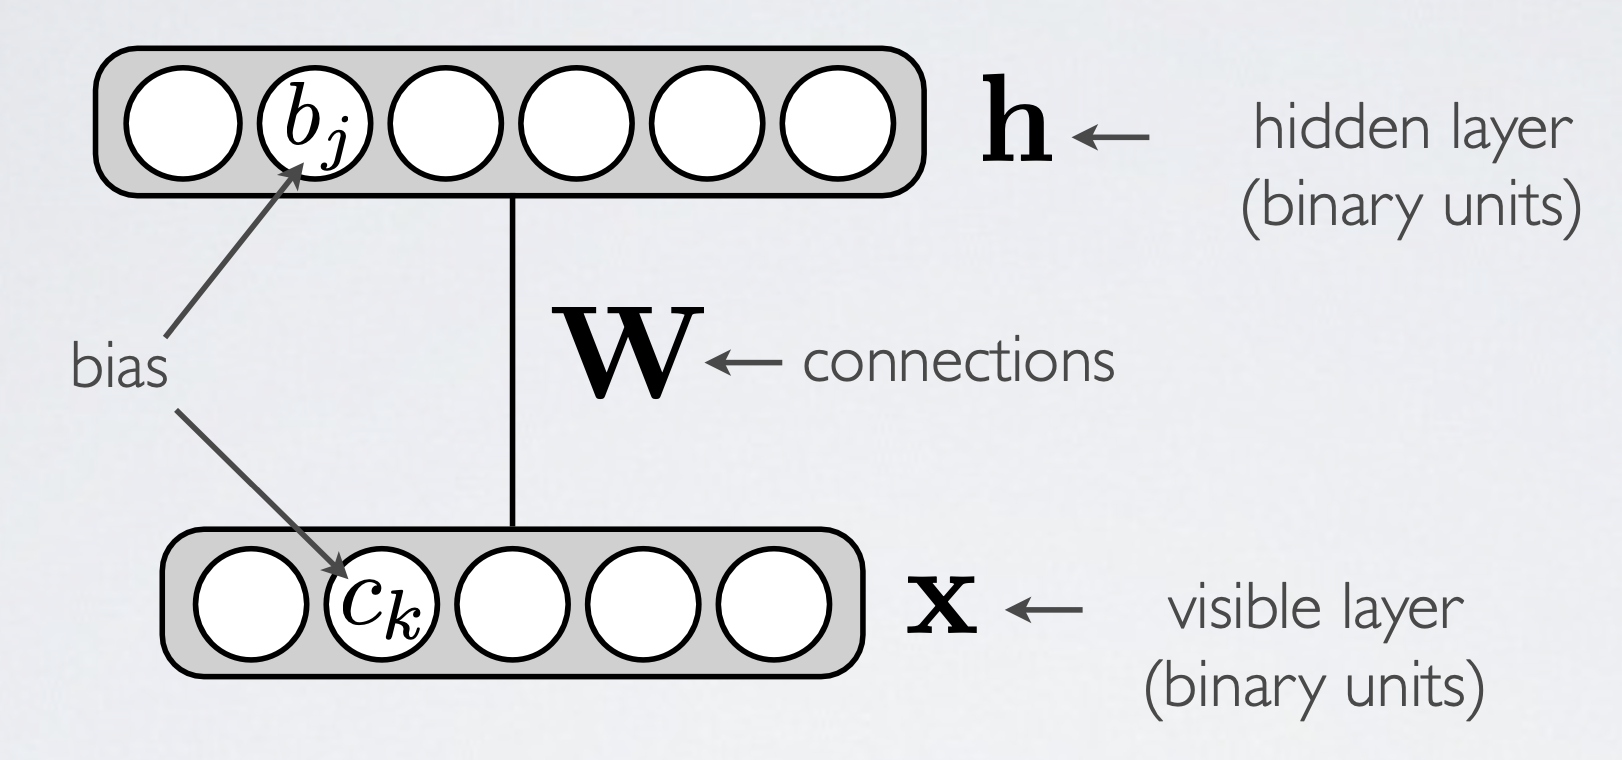
\includegraphics[width=0.4\textwidth]{Images/RBM.png}
    }
    \qquad
    \subfloat[\label{fig:l2}]{
    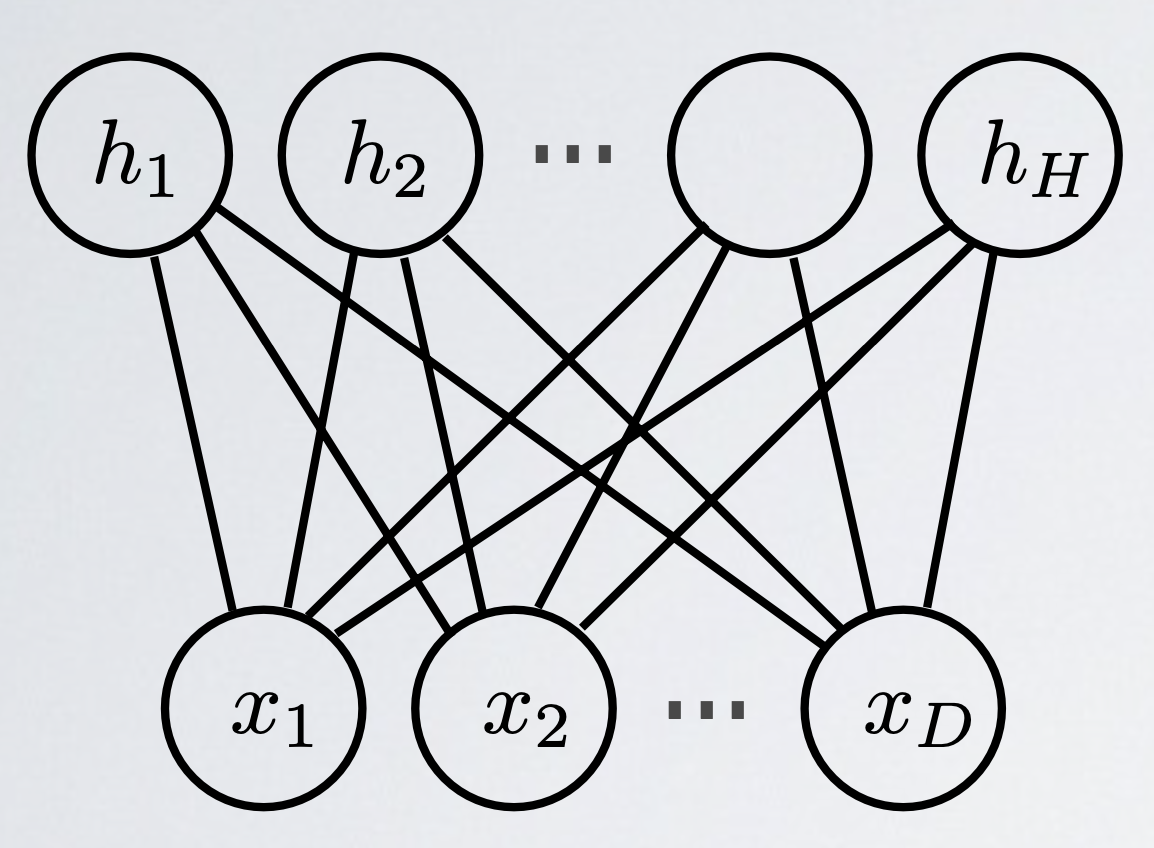
\includegraphics[width=0.3\textwidth]{Images/markovRBM.png}
    }
    \caption[RBM structure.]{Graphical representation of a Restricted Boltzmann Machine (a) and scalar representation of a RBM (b) \cite{hugo_larochelle_neural_2013}.}
\end{figure}
Before explaining what deep belief networks (DBNs) are, it is necessary to explain what Restricted Boltzmann Machines (RBMs) are. RBM can be regarded as a neural network for unsupervised machine learning. This means that they can autonomously extract meaningful features from the data. Mathematically, RBMs are networks made up of symmetrically coupled stochastic binary units. They are determined by a set of visible units $x_k\in[0,1]$, a set of hidden units $x_j\in[0,1]$, and connections between visible and hidden neurons. The RBms will define a distribution over $\mathbf{x}$ involving some latent stochastic variable corresponding to hidden units. Fig. \ref{fig:l1} shows a graphical representation of an RBM. The RBMs are characterized by the presence of an energy function described as
\begin{equation}
\begin{aligned}
E(\mathbf{x}, \mathbf{h}) & =-\mathbf{h}^{\top} \mathbf{W} \mathbf{x}-\mathbf{c}^{\top} \mathbf{x}-\mathbf{b}^{\top} \mathbf{h} \\
& =-\sum_j \sum_k W_{j, k} h_j x_k-\sum_k c_k x_k-\sum_j b_j h_j
\end{aligned}
\end{equation}
In a physical system, the distribution of a particular configuration of a variable of interest can be calculated as 
\begin{equation}
p(\mathbf{x}, \mathbf{h})=\exp (-E(\mathbf{x}, \mathbf{h})) / Z
\end{equation}
and $Z$ is a normalizing factor and is computed as 
\begin{equation}
Z=\sum_{\mathbf{v}, \mathbf{h}} e^{-E(\mathbf{v}, \mathbf{h})}
\end{equation}
The variable set $\theta=(\mathbf{w}, \mathbf{a}, \mathbf{b})$ is parameters to determine the RBM model, and the target of RBM training is to find the optimum $\theta^*$ that represents the training samples.
Suppose the bias $c_k$ is negative and the respective visible neuron $x_k$ equals one. In that case, the energy function will increase, and consequently, the probability of the visible neuron being equal to one will decrease. The network will attribute the zero state to neuron $x_k$. The opposite is also valid; the same applies to the bias $b_j$. The connection matrix $\mathbf{W}$, on the other hand, will help to consider the interaction between neurons. Indeed, if we represent the network in vector form as in Fig. \ref{fig:l2}, we can easily rewrite the probability distribution by highlighting the joint and single effects
\begin{equation}
p\left(\mathbf{x},\mathbf{h}\right) = \overbrace{\frac{1}{Z}\prod_j \prod_k \exp\left(W_{j,k}h_jX_k\right)}^\text{pair-wise factors} \quad \overbrace{\prod_j \exp\left(c_kx_k\right) \prod_k \exp\left(b_jh_j\right)}^\text{unitary factors}
\end{equation}
A typical example of RBMs use is in recommendation engines, where they are used as collaborative filters. Each visible neuron tells us whether a user will like a given content given another that he or she has liked. To better understand the potential of these networks, let us take the dataset of handwritten digits from the previous example as an example. Remember that each image is binary with dimensions \numproduct{16 x 16} pixels. After vectorizing the images, we define 256 visible neurons such that there is one neuron for each image pixel. We then move on to the training phase. Once the training phase is complete, we can take all the connections that join a hidden neuron to the visible neurons. We obtain a vector of connections $\mathbf{w} \in \mathbb{R}^256$ that we can rescale into a matrix $16 \times 16$ and interpret as an image. For each hidden neuron, we obtain an image like those in Fig. \ref{fig:minstbrm}. Let us now consider the matrix highlighted in red. Grey values are connections with weights close to zero, white values are positive, and black values are negative. This means that the hidden neuron has detected that the direction of the line indicated by the red arrow is a relevant feature for maximizing the representation capacity of the training dataset.
\begin{figure}
    \centering
    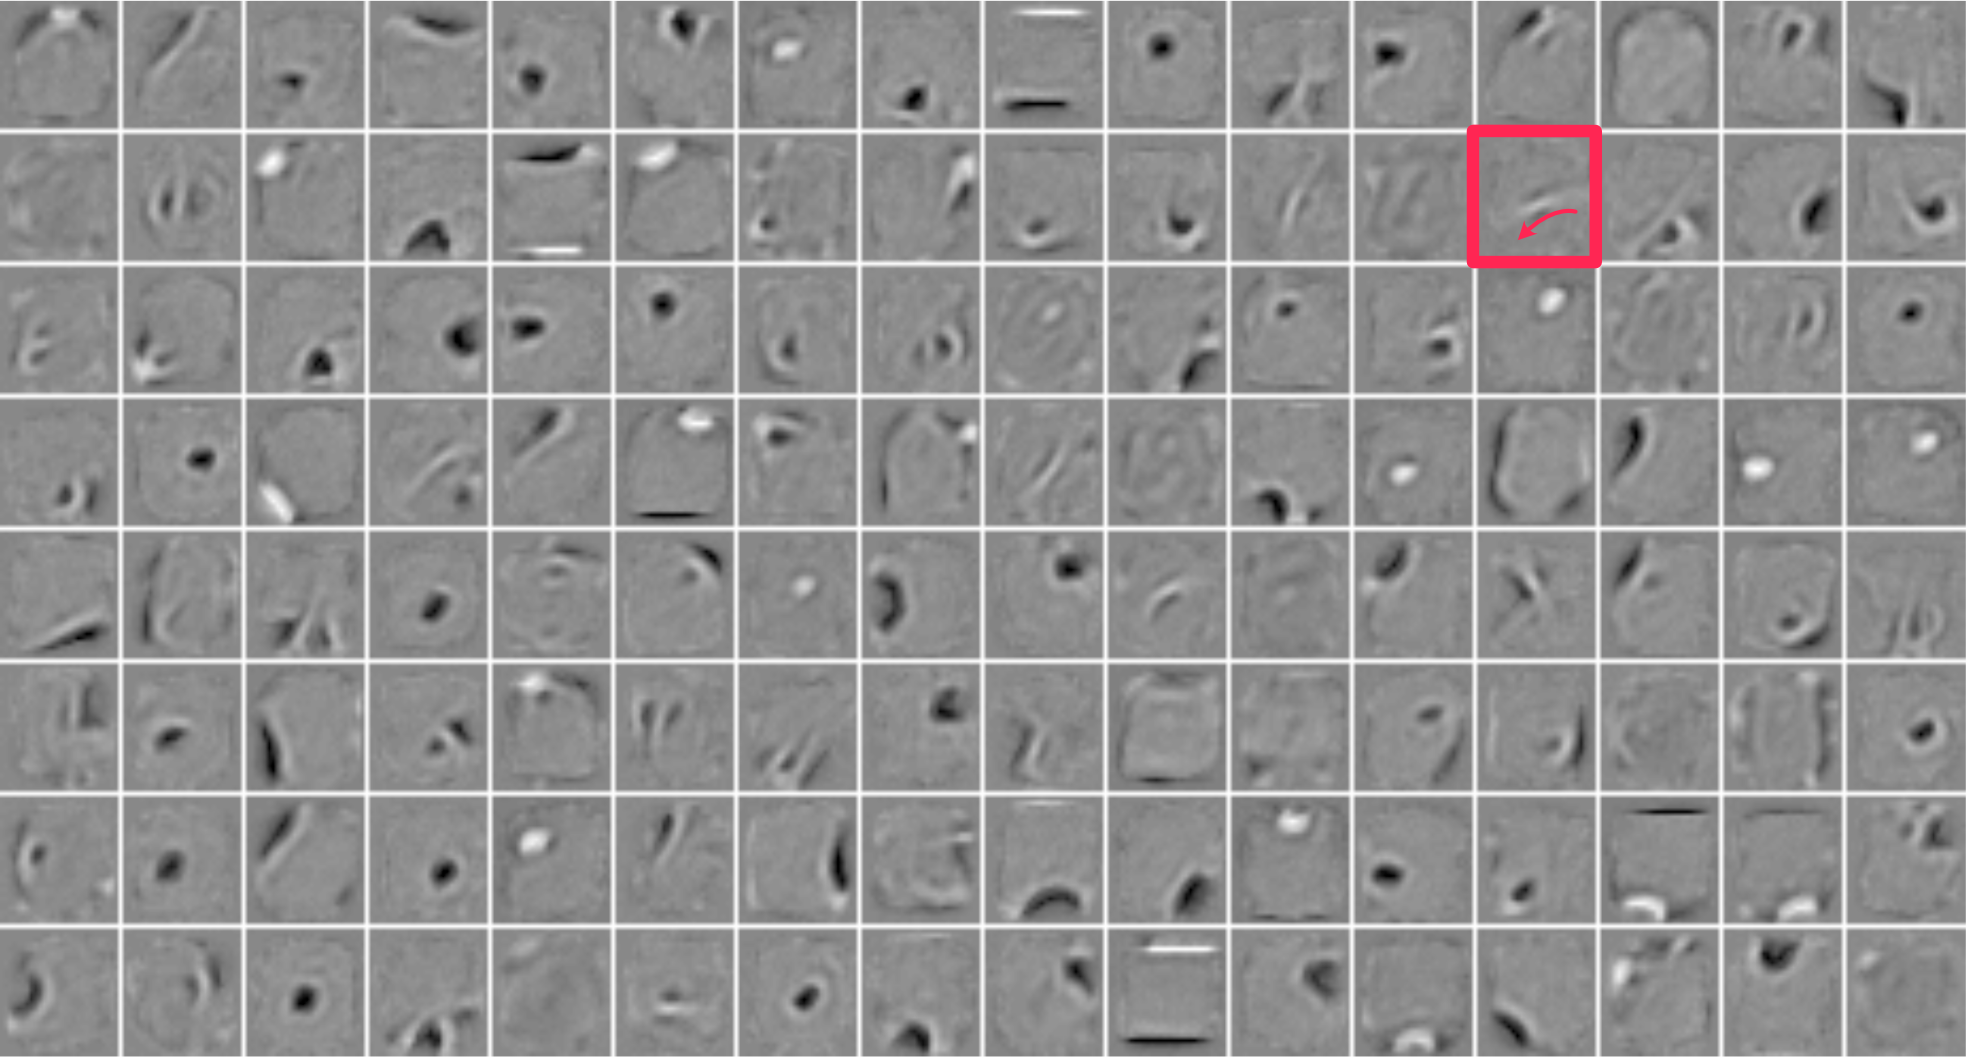
\includegraphics[width=0.7\textwidth]{Images/mnistrbm.png}
    \caption[RBM connection matrixes.]{Example of connections between visible and hidden neurons extracted from the handwritten digits dataset \cite{hugo_larochelle_neural_2013}.}
    \label{fig:minstbrm}
\end{figure}
A Deep Belief Network(DBN) is a powerful generative model that use a deep architecture of multiple stacks of Restricted Boltzmann machines(RBM). In particular, it is a generative model based on directed and undirected connections between nodes. The top 2 layers, in Fig. \ref{fig:dbnhugo}, the $\mathbf{h}^{(3)}$ and $\mathbf{h}^{(2)}$ layers are an RBM, while the other layers are layers of a Bayesian Network. This means that a conditional probability distribution with respect to the previous layer describes them. Indeed, the probabilistic distributions of these layers are
\begin{equation}
\begin{aligned}
p\left(h_j^{(1)}=1 \mid \mathbf{h}^{(2)}\right) & =\operatorname{sigm}\left(\mathbf{b}^{(1)}+\mathbf{W}^{(2)^{\top}} \mathbf{h}^{(2)}\right) \\
p\left(x_i=1 \mid \mathbf{h}^{(1)}\right) & =\operatorname{sigm}\left(\mathbf{b}^{(0)}+\mathbf{W}^{(1)^{\top}} \mathbf{h}^{(1)}\right)
\end{aligned}
\end{equation}
Recall that sigmoid functions $\operatorname{sigm}(z)$ is defined as
\begin{equation}
\operatorname{sigm}(z)=\frac{1}{(1+\exp (-z))}
\end{equation}
Since the distribution is defined by the sigmoid function, these layers are called sigmoid belief networks. The unique feature of DBNs is the ability to learn a hierarchical probabilistic model efficiently due to the level-by-level training that can be repeated several times. During the final phase of DBN training, all parameters found during the first unsupervised training phase are adjusted using a supervised learning technique using initial values obtained from the previous training stage.
\begin{figure}
    \centering
    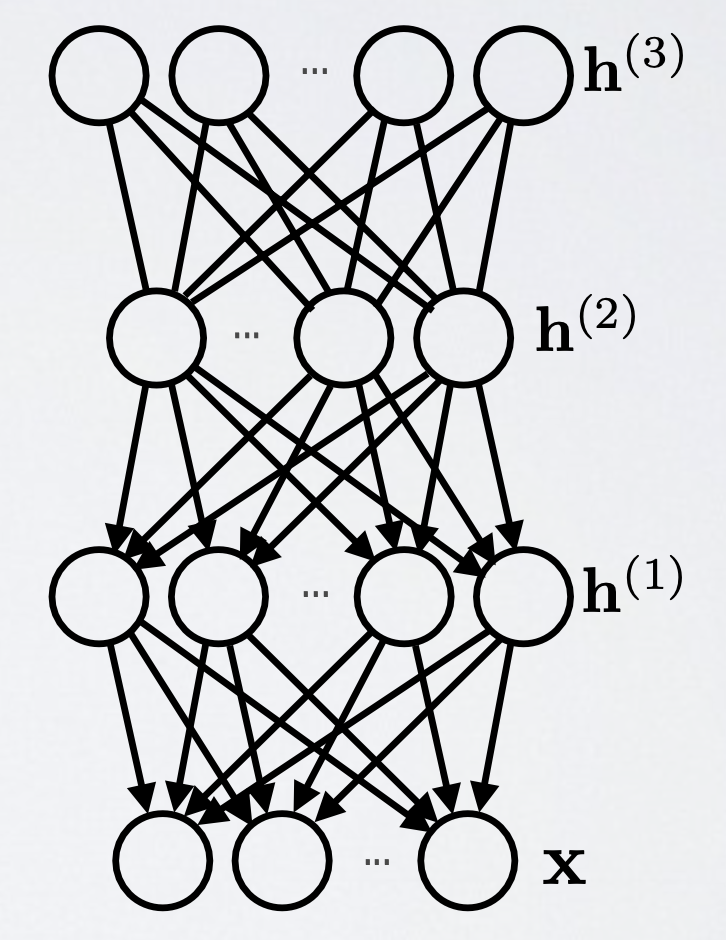
\includegraphics[width=0.25\textwidth]{Images/DBN graphical.png}
    \caption[DBN graphically represented.]{A graphical representation of a deep belief network \cite{hugo_larochelle_neural_2013}.}
    \label{fig:dbnhugo}
\end{figure}
% <<< End of Deep Belief Network

%%%%%
%%%%%

% Hot spot >>>
\section{Hot-Spot Detection Using ML Algorithm}
\label{sec:hotspotstateart}
This section will systematically review the literature on machine learning algorithms used for hot spot detection. The search strategy with the queries used, and the results are explained in detail in Appendix \ref{ap:research}. Table \ref{tab:slr} shows the papers selected for the literature review.
\begin{table}
\centering
\begin{tabular}{llllll}
\hline
\tiny
Author & \tiny
  Year & \tiny
  Process & \tiny
  Sensor & \tiny
  Proposed method & \tiny
  Reference \\ \hline 
  \tiny
\begin{tabular}[c]{@{}l@{}}Bugatti M.,\\ Colosimo B. M.\end{tabular} & \tiny
  2021 &
    \tiny L-PBF & \tiny
  \begin{tabular}[c]{@{}l@{}}High speed camera \\ (CMOS sensor)\end{tabular} &\tiny
  \begin{tabular}[c]{@{}l@{}}k-means FD clustering,\\ SVM, ANN\end{tabular} & \tiny \cite{bugatti_towards_2022}
   \\[0.3cm]
 \tiny \begin{tabular}[c]{@{}l@{}}Colosimo B. M.,\\ Grasso M\end{tabular} & \tiny
  2018 & \tiny
  L-PBF & \tiny
  \begin{tabular}[c]{@{}l@{}}High speed camera \\ (CMOS sensor)\end{tabular} & \tiny
  Weighted PCA & \tiny \cite{colosimo_spatially_2018}
   \\[0.4cm]
\tiny \begin{tabular}[c]{@{}l@{}}Yan H., \\ Grasso M, \\ Paynabar K.,\\ Colosimo B. M.\end{tabular} & \tiny
  2020 & \tiny
  L-PBF & \tiny
  \begin{tabular}[c]{@{}l@{}}High speed camera \\ (CMOS sensor)\end{tabular} & \tiny
  \begin{tabular}[c]{@{}l@{}}Penalized \\ spatio-temporal \\ regression\end{tabular} & \tiny \cite{yan_real-time_2021}
   \\[0.5cm]
\tiny \begin{tabular}[c]{@{}l@{}}Grasso M.,\\ Laguzza V.\\ Semeraro Q.,\\ Colosimo B. M.\end{tabular} &
  \tiny 2017 &
  \tiny L-PBF &
  \tiny \begin{tabular}[c]{@{}l@{}}High speed camera \\ (CMOS sensor)\end{tabular} & \tiny
  K-Means Clustering & \tiny \cite{grasso_-process_2017}
   \\[0.5cm]
\tiny \begin{tabular}[c]{@{}l@{}}Baumgartl H.,\\ Toma J.,\\ Buettner R., \\ Merkel M.\end{tabular} & \tiny
  2020 & \tiny
  L-PBF & \tiny
  Thermographic camera & \tiny
  CNN & \tiny \cite{baumgartl_deep_2020}
   \\[0.6cm]
\tiny \begin{tabular}[c]{@{}l@{}}Mao Y., Lin Hui, \\ Xuan Yu C., Frye R., \\ Beckett D., Anderson K., \\ Jacquemetton L., \\ Carter F., Gao Z., \\ Liao W. , Choudhary A. N., \\ Ehmann K., Agrawal A.\end{tabular} & \tiny
  2022 & \tiny
  L-PBF & \tiny
  Thermographic camera & \tiny
  CNN & \tiny \cite{mao_deep_2023}
   \\[1cm]
\tiny \begin{tabular}[c]{@{}l@{}}Ye D., \\ Soon Hong G., \\ Zhang Y., Zhu K., \\ Ying Hsi Fuh J.\end{tabular} &
  \tiny 2017 &
  \tiny L-PBF &
  \tiny \begin{tabular}[c]{@{}l@{}}Acoustic Sensor \\ (microphone)\end{tabular} &
  \tiny DBN & \tiny \cite{ye_defect_2018}
   \\[0.5cm] \hline
\end{tabular}
\caption{Summary of analyzed papers.}
\label{tab:slr}
\end{table}
Fortunately, many of these papers present methods that have been applied to the same dataset. Thus, we can compare different approaches and see how the different approaches perform on the same data obtained under the same conditions. All the analyzed papers propose approaches to HS detection in L-PBF processes. This is probably because, as mentioned above, collecting data for level 2 and level 3 process signatures is more difficult in EB-PBF processes, mainly due to the fact that external sensors are hard to install. Indeed, in L-PBF processes, it is easier to identify this type of anomaly as a more uniform pixel pitch characterizes the powder bed. Due to the high energy penetration within the metal material in EBM processes, the images show bright areas that interfere with measurement tasks. This causes several pre-processing operations to be required before analysis can take place \cite{grasso_powder_2020}. However, during the snowballing process described in Section \ref{sec:resmetodologies}, I found some examples of HS detection in EBM processes, which did not, however, use ML-based approaches. For example, in \citeauthor{grasso_powder_2020} (2020), the authors were able, using a high spatial resolution camera and a high temporal resolution camera, to calculate a summary index of the image to raise an alarm indicating the presence of a HS. This index exploits the anomalous behavior of the HS of the pixel intensity profiles. The HS presents a profile characterized by a high intensity maintained for a specific time interval and a subsequent slow cooling transitory. The synthetic index was computed as 
\begin{equation}
    \label{eq:sinteticgrassohs}
    S_I(x, y)=\sum_{t=0}^T \mathcal{I}\left( I_t(x, y) > k_1 \text{and} \Delta I(x, y<k_2 \right)
\end{equation}
where $\mathcal{I}(\cdot)$ is the indicator function, $I_t(x, y)$ is the pixel intensity of the $(x, y)$-th pixel in the $t$-th frame, $\Delta I(x, y)$ is the difference of $(x, y)$-th pixel intensities in the $t$-th and $(t-1)$-th frames and $k_1$ and $k_2$ are constants to be defined during a calibration phase. The authors also proposed a method for choosing $k_1$ and $k_2$ values, and for the data collected during the study, these values were set to 90\% and 10\%, respectively. The estimate of $S_I(x, y)$ can be iteratively updated as new video frames are acquired. The proposed algorithm is worthwhile for defect detection only and does not lead to any additional conclusion from temporal and spatial analysis.

We can now move on to the papers analyzed during the research of this thesis topic. In order to give as structured an approach as possible, papers are classified by the proposed method. This section follows the diagram in Fig. \ref{fig:SLRdiagramma}. This section will first illustrate machine learning methods and then deep learning approaches.
\begin{figure}
    \centering
    \subfloat[\label{fig:SLRdiagramma}]{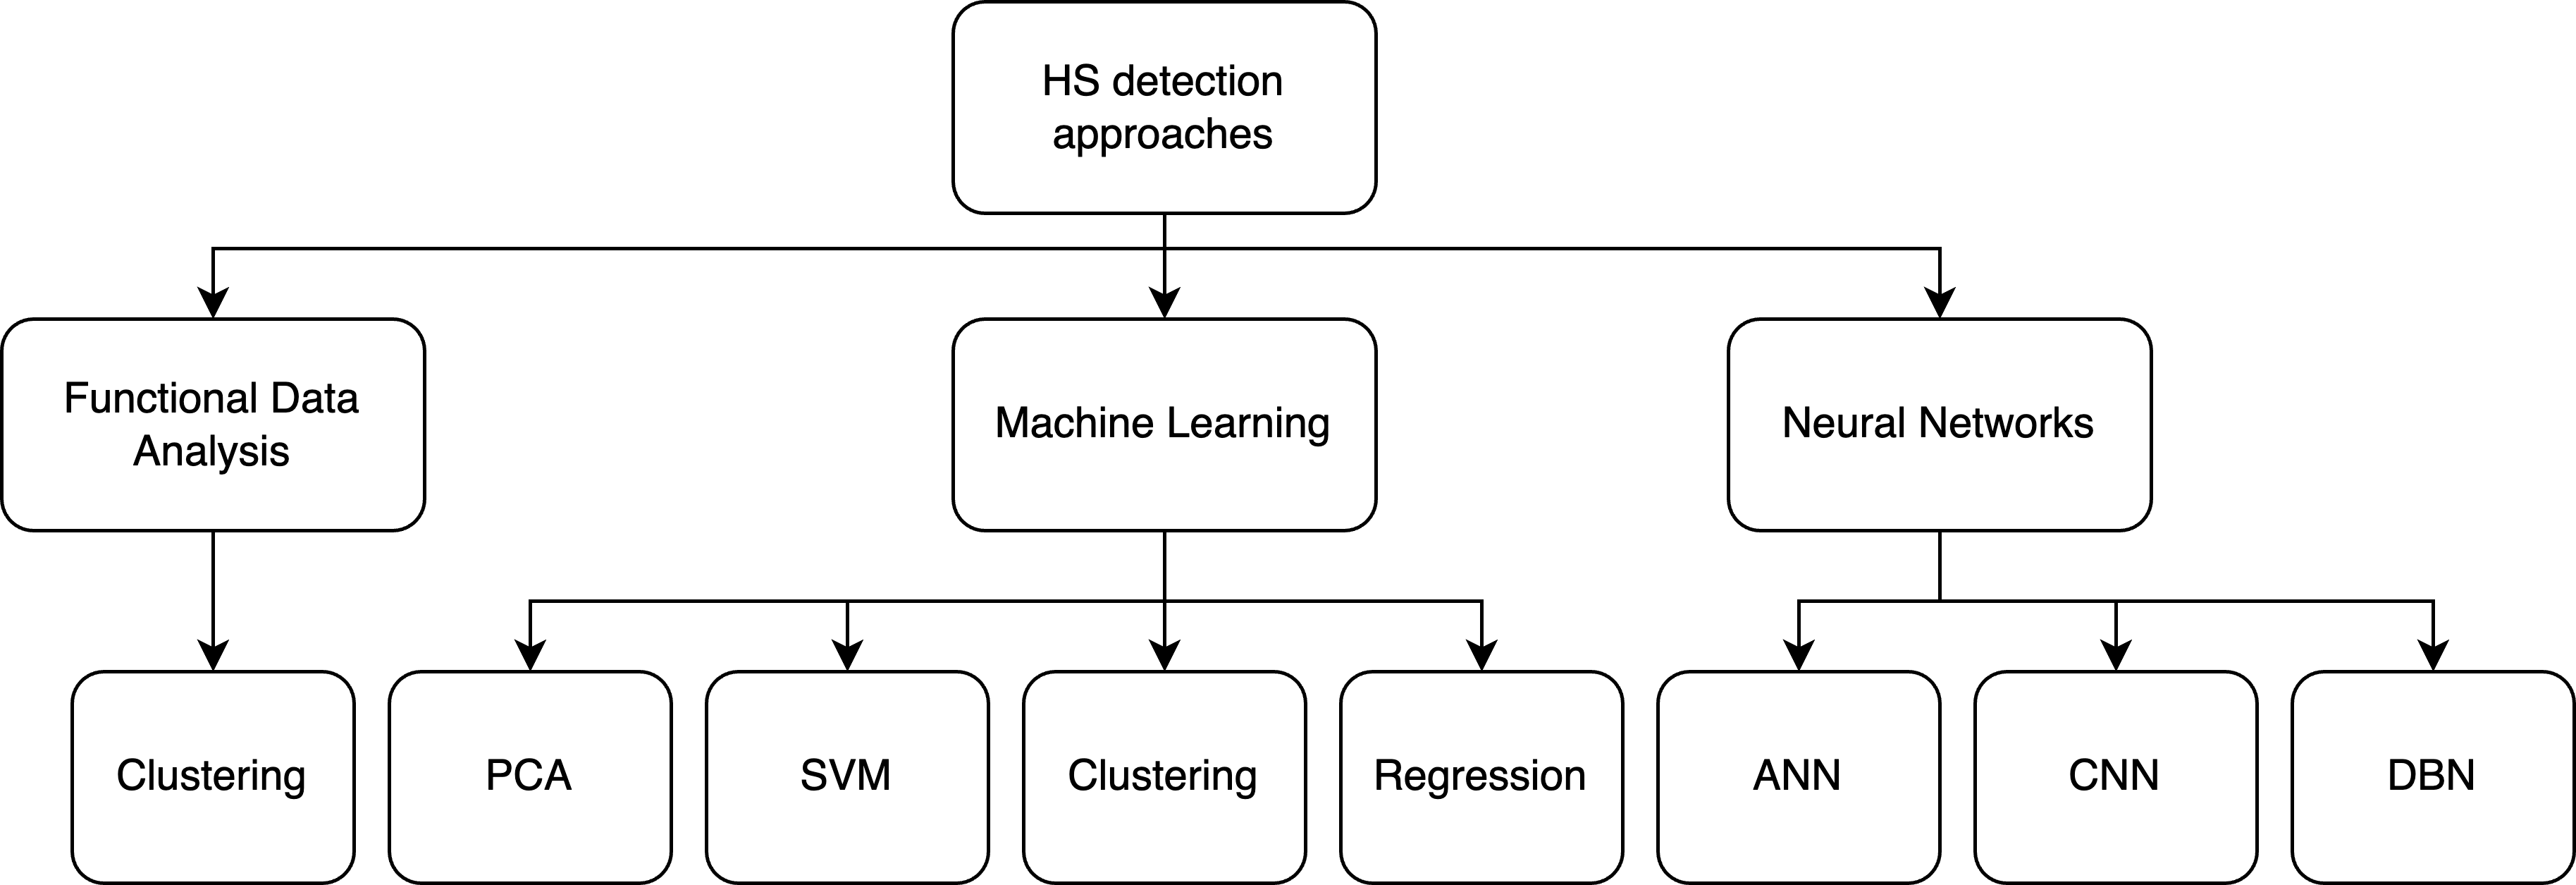
\includegraphics[scale=0.12]{Images/SLR diagram.png}}
    \qquad
    \subfloat[\label{fig:hsgrassoebm}]{
    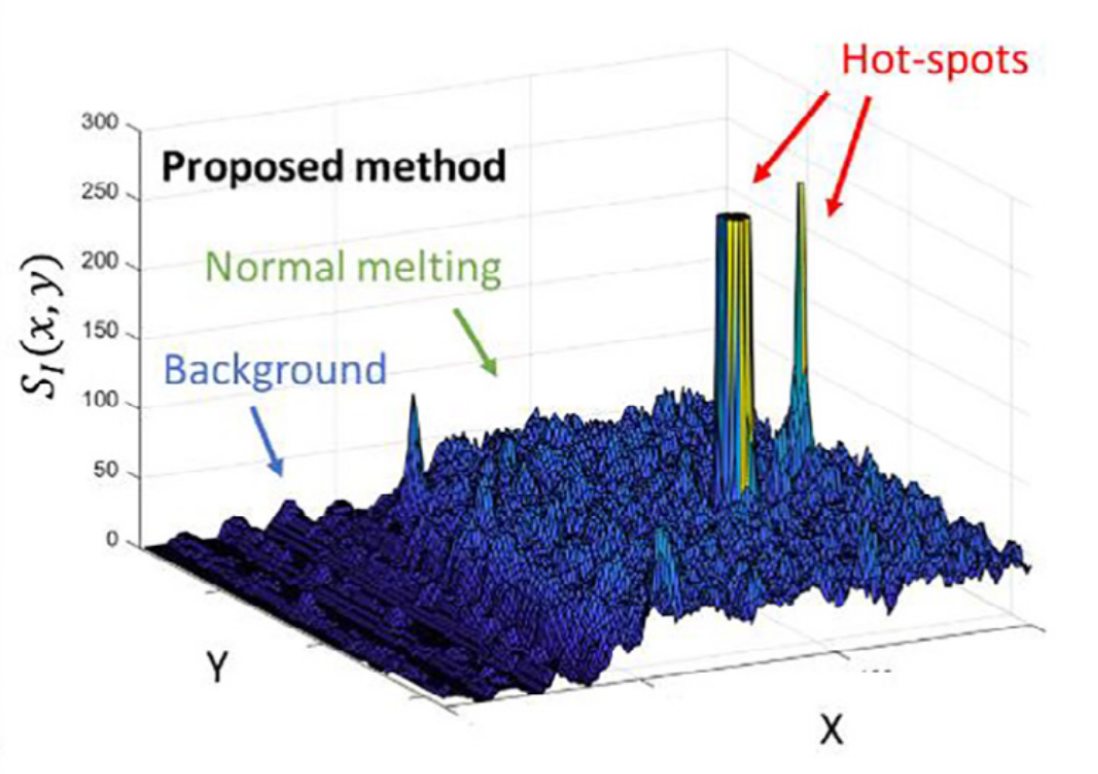
\includegraphics[width=0.4\textwidth]{Images/ebmgrassohs.png}}
    \qquad
    \subfloat[\label{fig:HSframes}]{
    \includegraphics[width=0.4\textwidth]{Images/framesPCAHS.png}
    }
    \caption[Hot spots detection.]{Breakdown of analyzed papers according to the approach used (a), hot-spot detection in EBM with synthetic index (b) \cite{grasso_powder_2020}, frames acquired for spatially weighted PCA (c) \cite{colosimo_spatially_2018}}
\end{figure}

\paragraph{PCA and Hotelling's $T^2$ distance.} In \citeauthor{grasso_-process_2017} (2017), authors proposed a method to perform in-process monitoring of an SLM process using image analysis. With this method, we are able to identify the spatial localization of local defects due to overheating phenomena. The proposed approach relies on PCA and Hotelling's $T^2$ distance in conjunction with an automated defect detection technique based on k-means clustering. Unlike some approaches we will see later, the peculiarity of this method is that it does not require any a priori ad-hoc segmentation, avoiding pre-processing operations such as thresholding. The authors printed the complex shape in Fig. \ref{fig:complexhs} measuring \numproduct{50x50x50} \unit{\milli\metre} using AISI 316 L powder via SLS. During the process, they acquired a video using an OlympusTM I-speed 3 camera (CMOS sensor) placed outside the build chamber viewport with an acquisition rate of 300fps. The acquired stream of gray-scale video images (Fig. \ref{fig:HSframes}) can be described in terms of a 3-dimensional array, $U=\left\{\boldsymbol{U}_1, \boldsymbol{U}_2, \ldots, \boldsymbol{U}_J\right\} \in \mathbb{R}^{J \times M \times N}$, where $M \times N$ is the size (in pixels) of each frame and $J$ is the total number of acquired frames over a time period of duration $T=J / f$, being $f$ the sampling frequency. $\boldsymbol{U}_j \in \mathbb{R}^{M \times N}$ is the $j$-th image, $j=1, \ldots, J$, and $\boldsymbol{u}_{m, n}=\left\{u_1(m,n), u_2(m, n), \ldots, u_J(m,n)\right\}$ is the intensity profile of the pixel at location $(m, n)$ over the $J$ acquired frames, with $n=1, \ldots, N$ and $m=1, \ldots, M$. The pixel intensity $u_j(m,n)$ ranges from 0 to 255, where 0 is black and 255 is white. Subsequently, individual frames were extracted from the video and vectorized in order to obtain a T-PCA. Thus, the three-dimensional array $\mathcal{U} \in \mathbb{R}^{J \times M \times N}$ is transformed into a matrix $\mathbf{X} \in \mathbb{R}^{p \times J}$, where $p=M \times N$. Each row of the matrix consists of a pixel intensity profile, i.e., the $1 \times J$ vector $\boldsymbol{u}(m, n)=\left[u_1(m, n), \ldots, u_J(m, n)\right]^{\mathrm{T}}$. The VPCA generates PCs that associate a weight to each frame. Hence, each PC is a $1 \times J$ vector that weights each time-location of pixel intensity profiles. Using a modified Hotelling distance, we can calculate a summary index for each pixel. The summary index will be calculated on the first $p$ PCs that describe at least 80\% of the total variance to characterize each pixel's behavior and identify single pixels (or spatial clusters of pixels) that exhibit anomalous intensity profiles. $T_l^2$ is computed as
\begin{equation}
T_l^2=\sum_{j=1}^m \frac{z_{l, j}^2}{\lambda_j} \quad(l=1, \ldots, p=M \times N)
\end{equation}
where $\lambda_j$ is the j-th eigenvalue of the PCA, and $z_{l, j}$ is the  projection of the $l$-th pixel on $j$-th frame intensity profile onto the $p$-dimensional PC orthogonal space. Recall that the projection is also called the score vector, and it is computed as
\begin{equation}
\mathbf{z}_l=\mathbf{V}^{\mathrm{T}}\left(\mathbf{x}_l-\overline{\mathbf{x}}\right)=\left[z_{l, 1}, \ldots, z_{l, J}\right]^{\mathrm{T}} \quad(l=1, \ldots, p=M \times N)
\end{equation}
where $\mathbf{V}$ is the orthonormal matrix whose $j$ th column, $\boldsymbol{v}_i$, is the $j$ th eigenvector of $\mathbf{S}^4$.
\begin{figure}
    \centering
    \subfloat[\label{fig:2kpca}]{\includegraphics[width = 0.75 \textwidth]{Images/2kPCA.png}}
    \qquad
    \subfloat[\label{fig:3kpca}]{
    \includegraphics[width = 0.75 \textwidth]{Images/3kPCA.png}}
    \caption[T-PCA approach for HS detection.]{Spatial distribution of $T^2(X,Y)$ (left), clusters identified using the kmeans approach (centre) and corresponding $D(k)$ statistics (right) for an in control layer (a) and for an OCC (b) \cite{grasso_-process_2017}.}
\end{figure}
In the paper mentioned above, the $T_l^2$ is a spatial indicator through the mapping $T_l^2 \in \mathbb{R}_{+}^p \rightarrow T^2(X, Y) \in \mathbb{R}_{+}^{M \times N}$. Hence, it can be represented in the same domain of original images, $T^2(X, Y)$, where $X$ and $Y$ denote the image pixel location. The spatial distribution of $T^2(X, Y)$ is, therefore, suitable to synthesize the information content of a video, represented in terms of a three-dimensional array, into a spatially distributed descriptor. After obtaining the distribution of the summary index over the image domain, we can move on to the automated defect detection technique based on k-means clustering. When applied to images or surface data, the K-means algorithm segments $k$ distinct areas characterized by a maximum within similarity. In this case, the algorithm is not applied directly to the pixels but to the values of the descriptor $T^2(X, Y)$, and each pixel is assigned to the closest centroid in terms of the Euclidean distance between the values of $T^2(X, Y)$. In the defect-free case, we expect to find two clusters in the image, the first corresponding to the background (loose powder) and the second to the trace left by the laser or the spatters emitted during fusion (foreground). If defects are present, we expect a third area to be identified. The proposed method consists of clustering the spatial distribution of $T^2$ with the aim of finding, according to a data-driven approach, the optimal number of clusters $k$. In the case where the optimal number of clusters $k>2$, we can raise an alarm. The most commonly used method for finding the optimal number of clusters is to identify a knee point in the graph of the sum of squared within-distances (SSWs) as a function of $k$. The SSWs are computed as 
\begin{equation}
\begin{aligned}
\operatorname{SSW}(k) & =(1 / k) \sum_{k=1}^K \sum_{i \in c_k}\left\|T_i^2(X, Y)_{c_k}-\overline{T^2}(X, Y)_{c_k}\right\| \\
k & =1,2, \ldots, K
\end{aligned}
\end{equation}
Computationally, to find the elbow of the graph, one calculates the distance $D(k)$ between SSW(k) and the straight line connecting the two extreme points of the graph, SSW(1) and SSW(K), and then selects the estimated optimal $\hat{k}$ corresponding to the maximum distance. Formally
\begin{equation}
\hat{k}=\operatorname{argmax}_k D(k)
\end{equation}
The authors also proposed a method to be able to use T-PCA within-layers. The method described so far has a drawback that could be a bottleneck for it to be applied in real-time. Indeed, we have to wait until the scanning phase is finished since we need all $J$ frames of the image stream. However, adopting a batch processing approach can speed up the computation. This method consists of starting to process frames from the same batch before they are collected. Let $\mathcal{U}_1 \in$ $\mathbb{R}^{J^{\prime} \times M \times N}$ be a first batch of $J^{\prime}$ frames such that $1<J^{\prime} \leq J$ and let $\mathbf{X}_1$ be its unfolded version. We can repeat these steps until the level scanning is complete. By analyzing the variance-covariance structure of these first $J^{\prime}$, we can check whether an alarm has occurred from frame $j=1$ up to frame $J^{\prime}$. The model can be updated when a new batch of frames $J^{\prime}$ is available, such that $2 J^{\prime} \leq J$. The spatial descriptor can also be updated, leading to a new spatial distribution, $T_2^2(X, Y)$, and an update of the clustering analysis. The method for automated defect detection allows alarms to be identified even during the update phase. In Fig. \ref{fig:2kpca}, we can see an example of a frame in control segmented into two clusters (in grey the spatter and the laser and in black the background), while in Fig. \ref{fig:3kpca} an example of a frame segmented into three areas (in red is marked the identified anomaly).

% SPATIALLY WEIGHTED
\paragraph{Spatially weighted PCA.} In \citeauthor{colosimo_spatially_2018} (2018), the authors proposed a method to detect HS by using a spatially weighted T-PCA (ST-PCA). We can consider this approach as an extension of the PCA approach described above. Indeed, if the T-PCA allows us to consider temporal dependence, the ST-PCA also allows us to consider spatial dependence. This is made possible by defining a matrix of spatial weights $\mathbf{W}$ of size $p\times p$ where $p = M \times N$. The $(k,h)$-th element quantifies the spatial dependency between the $k$-th and $h$-th pixels (the higher the value, the higher the dependency). To calculate the $\mathbf{W}$ matrix, three different approaches were proposed in the paper, hereafter called $W_1$, $W_2$ and $W_3$.
\begin{equation}
    \begin{gathered}
\mathrm{W}_1:\left\{w_{i, j}=\frac{1}{d_{i, j}^2}\right\} \\[0.3cm]
\mathrm{W}_2:\left\{w_{i, j}=1 \text { if } d_{i, j} \leq r, w_{i, j}=0 \text { otherwise }\right\} \\[0.3cm]
\mathrm{W}_3:\left\{w_{i, j}=\left(1-d_{i, j} / r^2\right)^2 \text { if } d_{i, j} \leq r, w_{i, j}=0 \text { otherwise }\right\}
\end{gathered}
\end{equation}
where $d_{i, j}$ is the Euclidean distance between the $i$-th \& $j$-th pixels of the image, and $r$ is a reference distance threshold. This threshold is used in calculating the $W_2$ and $W_3$ weights: these methods assign a weight equal to zero to all points with a distance greater than $r$. In the case of the above mentioned study, $r=5$. Then, the spatial weights matrix is used to penalize the spectral decomposition of the sample covariance matrix. Indeed, in the case of ST-PCA the variance-covariance matrix is defined as
\begin{equation}
    \mathbf{S}=  \frac{1}{p-1}(\mathbf{X}-\mathbbm{1} \overline{\mathbf{x}})^T \mathbf{W}(\mathbf{X}-\mathbbm{1} \overline{\mathbf{x}})
\end{equation}
where $\mathbf{X} \in \mathbb{R}^{\boldsymbol{p} \times \boldsymbol{J}}$ is the data matrix of the T-mode PCA formulation, $\overline{\mathbf{x}} \in \mathbb{R}^{1 \times J}$ is the sample mean vector and $\mathbbm{1}$ is a $p \times 1$ vector of ones.
\begin{figure}
    \centering
    \includegraphics[width = 0.8 \textwidth]{Images/ST-PCA vs T-PCA.png}
    \caption[ST-PCA compared to T-PCA]{Results of T-mode (upper panel) and ST-PCA (lower-panel) based methods with recursive updating \cite{colosimo_spatially_2018}.}
    \label{fig:tpcavsstpca}
\end{figure}
As in \citeauthor{grasso_-process_2017} (2017), the authors used the Hotelling's distance $T^2\in\mathbb{R}^{M\times N}$ and the automated rule for the identification of HS based on K-means clustering. Furthermore, they proposed two different methods to perform iterative updating of the ST-PCA so that it can also be used with non-stationary processes: the recursive updating approach (i) and the moving window updating approach (ii). The basic idea using approach (i) is to augment the data matrix by adding each new observed frame unless an OOC state is identified. Thus, given the fact that $\boldsymbol{X}_{1: p, 1: j}$ is the data matrix that includes $j$ frames when a new frame becomes available, it is augmented to $\mathbf{X}_{1: p, 1: j+1}$. Then, we can compute the new ST-PCA model. If the pattern of the resulting synthetic statistic, $T^2(m, n)$, is judged in control, the procedure is repeated for the following frame. Otherwise, an alarm is signaled. Approach (ii), however, involves keeping the temporal dimension $L$ of the data matrix fixed. Thus, once the first $L$ frames have been acquired, the oldest frame is discarded each time a new one is acquired. If the pattern of the resulting synthetic statistic, $T^2(m, n)$, is judged in control, the procedure is repeated for the following frame. Otherwise, an alarm is signaled. We can use this approach by applying it to individual frames or batches of frames. The last approach is a great way to make the algorithm more computationally efficient. However, the larger the batch size, the longer the delay with which an alarm is detected. The authors compared this new method with the method used in \citeauthor{grasso_-process_2017} (2017). From Fig. \ref{fig:tpcavsstpca}, we can see how this new one identifies areas previously classified as in control.
\begin{figure}
    \centering
    \includegraphics[width = \textwidth]{Images/firstcomp.png}
    \caption[ST-PCA simulation analysis results.]{Summary of simulation analysis results for three levels of simulated hot-spot size of $n=9$ (small), $n=20$ (medium) and $n=45$ (large) \cite{colosimo_spatially_2018}.}
    \label{fig:primocomparison}
\end{figure}
In Fig. \ref{fig:primocomparison}, we can see the different performances of the two proposed approaches as the size of the simulated defect, the method used to calculate the weights $w_{i, j}$, and the percentage of explained variance by the retained PCs vary. The simulation study was done by artificially altering the intensity of selected cross-shaped pixels of different sizes. From Fig. \ref{fig:primocomparison}, we can see how the ST-PCA outperforms the T-PCA in terms of ARL in all scenarios, sometimes even identifying defects that the previously proposed approach had not been able to detect. Recall that the ARL is the average run length, i.e., the number of frames before the defect is detected. Furthermore, we can appreciate how, in general, the approach for updating the ST-PCA based on the moving window of $L=50$ frames tends to outperform the recursive approach. This happens because the model's "memory" in terms of frames in the case of the moving window is shorter than the recursive updating approach. Therefore, it is more sensitive to OOC observations. Finally, we can see that the choice of methodology for calculating the weights $w_{i,j}$ is almost irrelevant in the case of the moving window. At the same time, the $W_2$ and $W_3$ methods are dominant with the recursive updating approach.

% REGRESSION
\paragraph{Spatio-temporal regression.} In \citeauthor{yan_real-time_2021} (2021), the authors proposed a penalized non-parametric regression model and recursive estimation algorithm so that the spatial and temporal correlation of defects could be taken into account. It is a highly-scalable spatio-temporal decomposition methodology to detect structured anomalies in real-time. The method is based on two common assumptions regarding HS events: natural events (in-control), such as the emission of plumes and spatters, are random in both the space and time domains, while HS events are localized in areas and consistent in space and time. Let $x_{s,t}$ be the pixel intensity at location $s$ and time $t$ we can then decompose it into the background $\mu_{s, t}$, a natural foreground event $u_{s, t}$, an anomaly foreground event $a_{s, t}$, and noise $e_{s, t}$ as
\begin{equation}
\label{eq:decreg}
x_{s, t}=\mu_{s, t}+u_{s, t}+a_{s, t}+e_{s, t}, \quad s=1, \ldots, S, \quad t=1, \ldots, T \text {, }
\end{equation}
where we assume that the background $\mu_{s, t}$ is known and $e_{s, t}$ follows an i.i.d normal distribution. However, $u_{s, t}$ and $a_{s, t}$ are unknown and should be estimated. We can model the anomaly as a first-order model with parameter $a_{s,t}=\theta_sx_{s,t-1}$. Substituting the relation just defined into Equation \ref{eq:decreg}, we obtain that
\begin{equation}
x_{s, t}=\theta_s x_{s, t-1}+\mu_{s, t}+u_{s, t}+e_{s, t}
\end{equation}
where $u_{s, t}$ and  $\theta_s$ are the parameters to be estimated. 
This parametric model was chosen after analyzing data from an observed HS phenomenon. As mentioned, in the presence of HS, the pixels show a higher and sustained intensity over time, characterized by a slow cooling phase. If we model the anomaly with an autoregressive model, we can capture the time dependence of the pixel with sustained intensity. Indeed, the cooling rate in normal conditions is so fast that the pixel intensity drops down to the background level from one frame to another, presenting as individual spikes. In the presence of HS, then, the parameter will be able to capture temporal autocorrelation, i.e., $\Theta_s \neq 0$ 
For the algorithm to be applicable in real-time, the estimation of these parameters must be data-driven. We can then estimate them with the penalized likelihood loss function:
\begin{equation}
\label{eq:likelihood}
\begin{aligned}
l_t\left(\boldsymbol{\theta},\left\{u_{s, t}\right\}_{s=1, \ldots, S}\right) & \\
= & \left(\sum_{s, t}\left\|x_{s, t}-\mu_{s, t}-u_{s, t}-\theta_s x_{s, t-1}\right\|^2+\gamma_1\left\|u_{s, t}\right\|_1\right)+ \\
& \quad+\gamma_2\|\boldsymbol{\theta}\|_1+\gamma_3\|\boldsymbol{\theta}\|_{T V}+\lambda_0\|\boldsymbol{\theta}\|^2
\end{aligned}
\end{equation}
where $\sum_{s, t}\left\|x_{s, t}-\mu_{s, t}-u_{s, t}-\theta_s x_{s, t-1}\right\|^2$ is the sum of squared errors and $\bm{\theta}=\left[\theta_1, \ldots, \theta_S\right]^{\prime}$. The penalties $\left\|u_{s, t}\right\|_1$ and $\|\boldsymbol{\theta}\|_1$ lead to the sparse estimation of natural and anomaly events, respectively. In order to be able to capture the spatial dependence as well, in Equation \ref{eq:likelihood} the term $||boldsymbol{\theta}||_{T V}=||\boldsymbol{D} \boldsymbol{\theta}\|_1$ was added, where $\boldsymbol{D}$ is defined as
\begin{equation*}
    \boldsymbol{D}=\left[\begin{array}{cccc}
1 & -1 & & \\
& \ddots & \ddots & \\
& & 1 & -1
\end{array}\right]
\end{equation*}
Finally, also in Equation \ref{eq:likelihood}, the term $\lambda_0\|boldsymbol{\theta}|^2$ was also added to make the stoma more robust and ensure that large background areas are characterized by the same pixel intensity even in different frames. At each instant of time, it will be necessary to solve the equation
\begin{equation}
\label{eq:casinominimal}
\begin{gathered}
\min _{\left\{u_{s, t}\right\}} L\left(\boldsymbol{\theta},\left\{u_{s, t}\right\}_{s=1, \ldots,} s, t=1, \ldots, T\right) \\
=\sum_{t=1}^T \lambda^{T-t} l_t\left(\boldsymbol{\theta},\left\{u_{s, t}\right\}_{s=1, \ldots,} s\right)
\end{gathered}
\end{equation}
to identify the anomalies $\bm{\theta}$. Parameter $\lambda \in (0,1)$ is used to give more importance to the most recent data. Since Equation \ref{eq:casinominimal} must be computed recurrently, the authors proposed an algorithm called ADMM to update it computationally efficiently. As explained earlier, in the case where two pixels are not autocorrelated, we will have $\theta_s=0$, so to identify the presence of anomalous pixels, we must at each instant of time perform the following hypothesis test:
\begin{equation}
H_0: \boldsymbol{\theta}=0 \qquad H_1: \boldsymbol{\theta}=\delta \hat{\boldsymbol{\theta}}_{\gamma_2, \gamma_3}(t)
\end{equation}
We can compute the test statistics as 
\begin{equation}
\tilde{T}_{\gamma_2, \gamma_3}(t)=\frac{\left(\left(\hat{\boldsymbol{\theta}}_{\gamma_2, \gamma_3}(t)\right)^{\top} \boldsymbol{\theta}_{0,0}(t)\right)^2}{\left\|\hat{\boldsymbol{\theta}}_{\gamma_2, \gamma_3}(t)\right\|^2} 
\end{equation}
Before $\tilde{\boldsymbol{T}}_{\gamma_2, \gamma_3}$ can be used for process monitoring, the regularization $\gamma_2, \gamma_3$ should be chosen carefully, as it plays an important role in controlling the sparsity and smoothness of $\hat{\boldsymbol{\theta}}_{\gamma_2, \gamma_3}$. To make the testing statistics robust to tuning parameter selection authors proposed a modified statistic:
\begin{equation}
\tilde{T}(t)=\max _{\left(\gamma_1, \gamma_2, \gamma_3\right) \in \Gamma} \frac{\tilde{T}_{\gamma_2, \gamma_3}(t)-E\left(\tilde{T}_{\gamma_2, \gamma_3}\right)}{\sqrt{\operatorname{Var}\left(\tilde{T}_{\gamma_2, \gamma_3}\right)}}
\end{equation}
Here, the mean and variance of the $\tilde{T}_{\gamma_2, \gamma_3}$ can be estimated by the sample mean and sample variance of $\tilde{T}_{\gamma_2, \gamma_3}$ from the In-Control (IC) data. By defininig control limit $L>0$ to reach a desired ARL. If $\tilde{T}(t)>L$, the monitoring scheme would trigger an alarm. Finally, by looking at the non-zero $\boldsymbol{\theta}$ components, we can identify the area where the defect occurred. The proposed method has a computational time of about $1/30$ compared with the computational time of ST-PCA, and also has a much lower ARL, as can be seen from the table \ref{tab:last}.
\begin{table}
\small
\centering
\begin{tabular}{llllll}
\hline
\rowcolor{bluepoli!40}
Hot-spot size & \multicolumn{1}{c}{Method} & \multicolumn{1}{c}{ARL} & \multicolumn{1}{c}{Precision} & \multicolumn{1}{c}{Recall} & F-score\\
\hline \hline
\\
Small & Regression & 3.39(1.57) & 0.88(0.27) & 0.98(0.14) & 0.90(0.24) \\
$(n=4)$ & PCA & 87.66(49.48) & 0.00(0.01) & 0.30(0.43) & 0.01(0.01) \\
& ST-PCA & 73.19(1.57) & 1.00(0) & 1.00(0) & 1.00(0) \\[0.5 cm]
Medium & Regression & 2.29(0.78)& 0.97(0.11)& 0.99(0.10)& 0.98(0.10) \\
$(n=20)$& PCA& 84.81(47.61)& 0.02(0.03)& 0.31(0.43)& 0.04(0.06) \\
& ST-PCA& 65.76(2.07)& 0.83(0.01)& 0.96(0.01)& 0.89(0.01) \\[0.5 cm]
Large& Regression& 1.20(0.58)& 0.87(0.16)& 0.99(0.10)& 0.92(0.13) \\
$(n=80)$& PCA& 74.50(53.21)& 0.12(0.14)& 0.46(0.47)& 0.19(0.21) \\
& ST-PCA& 65.76(2.07)& 0.83(0.01)& 0.96(0.01)& 0.89(0.01) \\[0.5 cm]
\end{tabular}
\caption{Performances of spatio-temporal regression compared to PCA and ST-PCA. For different simulated HS sizes, are reported ARL, precision, recal and F-score, both the mean value and the standard deviation between parenthesis on multiple simulations \cite{yan_real-time_2021}.}
\label{tab:last}
\end{table}
\textcolor{red}{Manca ancora le considerazioni e le comparazione di tutti gli altri metodi. Manca anche la definizione di precision recall e F-score.}




% FUNCTIONAL DATA CLUSTERING
\paragraph{Clustering of Functional Data.} In \citeauthor{bugatti_towards_2022} (2022), the authors systematically proposed and compared different methods to identify hot spots in L-PBF processes. The dataset used is the same as in previous papers, based on ST-PCA and T-PCA conjuncted with Hotelling's distance. Please recall that Section \ref{sec:hotspot} shows an example of the complex shape. The authors systematically proposed and compared different methods to identify hot spots in L-PBF processes. In particular, all the algorithms presented in the report use the same algorithm for data extraction based on three simple steps:
\begin{enumerate}
    \item Apply a threshold to video frames to identify bright areas. The threshold was an arbitrary value of 200;
    \item Pixels within each bright region are isolated;
    \item The average brightness of the pixels in each isolated region is extracted for the subsequent $L$ frames. In this way, a time series is obtained. In the study, the authors set the parameter for the "memory" of the average to $L=10$.
\end{enumerate} the author proposed an approach based on k-means clustering of functional data, a version of the much more popular k-means clustering algorithm we saw earlier. In this case, however, we are not interested in finding simple centroids but functional centroids. Section \ref{sec:fda} will provide an in-depth description of functional data. For now, it is enough to know that functional data are data that, despite being discrete, we can assume some unknown function generated the observations. Therefore, Functional data are not stochastic variables but observations of an unknown mathematical function perturbed by a random error. Thus, let $X=\left\{x_1, x_2, \ldots, x_n\right\}$ be a given functional dataset of size $n$ to be analyzed, where $x_i$ belongs to $\mathbb{R}^m$, and $V=\left\{v_1, v_2, \ldots, v_c\right\}$ be the functional set of cluster centers, where $c$ is the number of clusters and $v_i$ belongs to $\mathbb{R}^m$. To implement this technique, although it is not common practice for this type of clustering algorithm, only two clusters were superimposed, i.e., normal and anomalous regions. The result of this algorithm is two functional data centroids, one associated with in-control and one associated with the presence of an HS. In this case, a further pre-processing step was performed to improve classification: to prevent the brightness of the pixels from starting to increase after the decay phase (perhaps due to consecutive scans), authors applied the transformation $b_{a d j}(t+1)=\min (b(t), b(t+1))$, where $b(t)$ is the brightness of the pixel at time $t$.

\begin{figure}
    \centering
    \subfloat[\label{fig:SVMHS}]{
        \includegraphics[width=0.4\textwidth]{Images/SVMHS.png}
    }
    \qquad
    \subfloat[\label{fig:NNHS}]{
        \includegraphics[width=0.35\textwidth]{Images/NNHS.png}
    }
    \caption[HS detection methods.]{Result of the K-mean functional data clustering algorithm (a), the optimal separating hyperplane in SVM (b), fully connected NN used to perform binary classification (c)\cite{bugatti_towards_2022}.}
\end{figure}


% SUPPORT VECTOR MACHINE
\paragraph{Support Vector Machine} Also, in \citeauthor{bugatti_towards_2022} (2022),
authors proposed a method to defect classification based on the use of a supervised machine learning technique called support vector machine (SVM). SVM is a machine learning technique that identifies the hyperplane between the two classes to optimize their separation. The most significant advantage of this technique is that it does not require any assumptions about the distribution of the data used as input, so it is a method that can also be applied to datasets with large dimensionality but few observations. However, this technique has a significant drawback due to its very nature: it requires labeled data for the training phase. For this reason, to avoid excessive human bias, all bright regions whose centroid lay in the acute corner area were found defective after final inspection and labeled hot-spots. Another drawback of SVM is the need to have multivariate data as input. Some SVM approaches applied to functional data have been proposed, but they are still at an 'experimental' stage, and there is no ready-to-use code routine. Hence, the authors decided to perform some feature extraction in order to be able to process multivariate data. In particular, the authors proposed to extract for each functional dataset two features:
\begin{itemize}
    \item Mean gradient
    \begin{equation}
        \overline{\Delta_1 b}=\frac{1}{L-1} \sum_{t=1}^{L-1} \Delta_1 b(t)=\frac{1}{L-1} \sum_{t=1}^{L-1}(b(t+1)-b(t))
    \end{equation}
    \item Maximum mean brightness drop between consecutive frames
\begin{equation}
    \Delta_{1, \text { max }} b=\max _{1 \leq t<L} \Delta_1 b(t)
\end{equation}
\end{itemize}
In addition, the shape and size of the bright area were also added as input data. In Fig. \ref{fig:SVMHS}, there is a graphical representation of the optimal separating hyperplane.




% DEEP LEARNING METHODs.
\paragraph{Deep learning methods.} HS detection methods using neural networks are much easier to understand and require less explanation, especially those using CNNs. Also, in \citeauthor{bugatti_towards_2022} (2022), authors proposed a method based on an NN to implement a supervised classification algorithm that finds the optimal non-linear combination of input variables to distinguish between two classes. A fully connected NN is a NN in which all neutrals are connected. In this case, since it is a binary classification problem, the output neuron will have a sigmoid activation function, and the numerical output can be seen as the probability of belonging to the success class. Like the SVM, the NN does not require any a priori assumptions about the input data distribution but requires labeled data for the training phase. For this reason, the clustered dataset using k-means clustering of functional data was used as input. The main advantage of NNs over SVM is that it does not require extracting features a priori, but NNs learn autonomously which features are significant. It will have as input the functional data extracted from the video. By doing so, we are sure to introduce no human bias and have no loss of information due to choosing the wrong feature. However, in this way, we cannot control the features extracted from the neural network. We will see in a few that by using CNNs it is possible to obtain a heat map of feature importance. For the NN-based approach to be comparable with the SVM approach, additional information about the shape and size of the identified bright regions was also given as input. The number of hidden layers and their size were treated as hyper-parameters during the choice of the network structure. Fig. \ref{fig:NNHS} presents the structure of the final NN. In \citeauthor{baumgartl_deep_2020} (2020), the authors monitored an L-PBF process with H13 material using a thermographic camera to acquire data. The camera was a PYROVIEW 640G/50 Hz/\ang{25} $\times$ \ang{19}/compact + (DIAS Infrared GmbH, Dresden, Germany), with a spectral range of \SIrange{4.8}{5.2}{\micro\metre} and an optical resolution of \numproduct{640 x 480} pixels. The acquisition frequency was set at \SI{50}{fps}. This measurement setup is a standard procedure for material analysis and process optimization. It is important to notice that this method was used for large hot spots, more similar to the so-called 'residual heat' effect that we have seen in Section \ref{sec:hotspot}. CNN has been used to classify defects from a large area characterized by prolonged overheating. The output classes used by the authors are 3: delamination, splatters, and OK (in-control). However, considering the excellent results obtained (accuracy of 97.87\% with an STD of 0.93\%), it is interesting to show the neural network structure used. In Fig. \ref{fig:cnnresidual}, there is the architecture of the final model.
\begin{figure}
    \centering
    \includegraphics[scale=0.5]{Images/CNN residual heat.png}
    \caption[CNN for residual heat.]{Model architecture of the CNN for thermal data \cite{baumgartl_deep_2020}.}
    \label{fig:cnnresidual}
\end{figure}
We can also see that there are some layers we still need to discuss: the depthwise-separable convolutions. Unlike classical convolutional networks, these layers are used to learn one feature at a time. In fact, in classical CNNs, the kernel must learn spatial features and cross-channel features simultaneously. For example, with depthwise separable convolutions, we can use a 1x1 convolution layer for summarising the red-green-blue channels in a single mixed color channel and only then use a 3x3 or 5x5 convolution layer to extract the spatial features. This approach is mainly used to reduce the computational cost. Finally, with this CNN, the authors could calculate activation heatmaps. These heat maps indicate the importance of spatial features for each class. Thus, although it is a black-box model, it is somewhat interpretable. However, we cannot capture time behavior with this approach since it is based on single video frames.

% DEEP BELIEF NETWORK
\paragraph{Deep belief network.}
\begin{figure}
    \centering
    \subfloat[\label{fig:acoustic_dbn_ok}]{\includegraphics[width=0.65 \textwidth]{Images/dbnacoustic.png}}
    \quad
    \subfloat[\label{fig:acoustic_dbn_ooc}]{\includegraphics[width=0.65 \textwidth]{Images/defectacoustic.png}}
    \caption[Acoustics process signatures.]{Example of an acoustic signature of an in-control process (in red environmental acoustic profile) (a) and two defective acoustic signatures, one for a overheating defect (left) and one for an extreme overheating (right) (b) \cite{ye_defect_2018}.}    
\end{figure}
In \citeauthor{ye_defect_2018} (2018), authors used the acoustic signatures of the process to identify and classify five different fault categories: balling (A), slight balling (B), normal (C), slight overheating (D), and overheating (E). The air-borne acoustic signatures collected for the experiment result from plasma fluctuation during the SLS process. Underheating or overheating over metal powder by laser processing is characterized by dynamic plasma variation, leading to different acoustic profiles. In SLS, plasma is generated when highly concentrated energy irradiates the vapors that develop during printing. The air density is collected near the melting area since it is determined by the dynamics of the plasma density $N_P$. Furthermore, variations in the plasma density cause the atmospheric pressure value around the printing area to fluctuate. The acoustic intensity captured by the microphone can be calculated as
\begin{equation}
I = \frac{P^2}{f(N_P)\nu}
\end{equation}
where $P$ is the pressure, $f(N_P)$ is the air density as a function of the plasma density, and $\nu$ is the speed of sound. To acquire the acoustic signals, the authors used a microphone fixed at an angle of 30° over the platform, characterized by a frequency response from 0 Hz to 100 kHz. The sampling frequency used was 200kHz. In Fig. \ref{fig:acoustic_dbn_ok}, we can see an example of an acoustic signature of the process during the printing process (blue) and without the melting, represented both in the time domain and the frequency domain. The acoustic signature collected without melting is mainly from the machine operating and environmental noise. In Fig. \ref{fig:acoustic_dbn_ooc}, two acoustic signatures for class E and D defects can be seen. For the classification of acoustic profiles, the authors proposed using a DBN like the one in Fig. \ref{fig:dbnhsgrafica}. The training consists of five successive stages:
\begin{enumerate}
\item Train the first layer as an RBM that models the raw (frequency domain) input $\mathbf{v}=x(f)$ as its visible layer. 
\item Use that first layer to obtain a representation of the input that will be used as data for the second layer. In this case, it is the mean activations $P(\mathbf{h}^1 =1\mid\mathbf{v})$.
\item Train the second layer as an RBM, taking the transformed data as the visible layer of that RBM. 
\item Iterate 2 and 3 for the desired number of layers, each time propagating upward either samples or mean values. 
\item Fine-tune all the parameters of this deep architecture using a supervised machine learning approach for DBN.
\end{enumerate}
Overall, they achieved a classification rate of 93\%, which increased to 93.63\% after data noise reduction. It is important to note that if the data used represents the acoustic signature in the frequency domain obtained by fast Fourier transform, the classification rate increases by more than 20 percentage points. The classification rate of acoustic profiles in the time domain is about 70\%. The authors demonstrated that the proposed approach can outperform the SVM algorithm and the classical NNs. Furthermore, the advantage of this approach is that it does not require any preprocessing or feature extraction of the acquired signals, and by analyzing the connections of the RBM part, fundamental features in the classification can be understood (ed.), which could also be used in other methods.

\begin{figure}
    \centering
    \includegraphics[scale=0.5]{Images/DBN paper.png}
    \caption[DBN used to detect HS.]{A graphical representation of the DBN used by the authors in \cite{ye_defect_2018}.}
    \label{fig:dbnhsgrafica}
\end{figure}


% Other methods
\paragraph{Other methods.} Furthermore, although it is beyond the scope of this thesis, it is worth mentioning that digital twins have been used in recent years in the scope of quality control. A digital twin is a model built using data streams to create a digital representation of a real-world asset to improve collaboration, information access, and decision-making. In other words, it combines simulation technology and real-time data. Using this technology, we can see when the printing process deviates from the simulated process and identify which process parameters to change to return to a normal condition.
% <<< End of Hot spot 
% <<< end of PBF Hot Spot State of the Art


% Proposed method Bagging Voronoi >>>
\chapter{Bagging Voronoi Clustering Algorithm}
\label{ch:baggingvoronoi}
As discussed in the previous chapter, most of the solutions found in the literature rely on deep learning models. However, these models have a significant drawback: they are very complex and with a lot of parameters, meaning they excel at predicting the model's output, but are not equally suitable for explaining the phenomenon. Indeed, deep learning model can be seen as black-box model. We can use packages such as Shap, shown in Fig. \ref{fig:shap}, available as a Python package. SHAP (SHapley Additive exPlanations) utilizes game theory principles to explain the outputs of any machine learning model. It bridges the gap between optimal contribution distribution and localized explanations by employing the traditional Shapley values from game theory, along with their associated extensions as described by \citeauthor{lundberg_unified_2017} (2017).
\begin{figure}
    \centering
    \includegraphics[width=0.7\textwidth]{Images/shap.png}
    \caption[SHAP python package.]{Example of the SHAP python package \cite{scott_lundberg_shap_2023}.}
    \label{fig:shap}
\end{figure}

In this section, I will propose an approach for clustering areas within the printing plate with anomalous behaviours. With this approach, we should be able to clustering temperature profiles that exhibit a similar behaviour considering also the distance in the printing plane. This analysis can be done pixel-wise, window-wise or, in the case of a lattice structure, cell-wise. "In general, it can be applied to any functional data referenced by a lattice in $\mathbb{R}$, $\mathbb{R}^2$ or $\mathbb{R}^3$. This algorithm is based on functional data. The analysis of functional data allows us to gain a comprehensive and detailed understanding of the anomalies, which would enable us to discern if there are specific zones on the print plane behaving irregularly and to understand how hot spots might influence the mechanical properties of the printed part, given the fact that we have a functional knowledge of those phenomena. In Section \ref{sec:fda}, I will provide a brief introduction to functional data analysis, in Section \ref{sec:bvc}, I will provide a detailed explanation of the Bagging Voronoi algorithm proposed by \citeauthor{secchi_bagging_2013} for functional data clustering and, in Section \ref{sec:bcv-cases} I will present three successful case studies of algorithm application.

% Functional Data Analysis >>>
\section{Functional Data Analysis}
\label{sec:fda}
\textbf{\textcolor{red}{To be completed.}}
\\
%In the Indeed, functional data analysis (FDA) is a branch of statistics that deals with data represented as functions. Instead of observing data at a set of fixed points, as is common in traditional statistics, FDA focuses on data that comes in the form of curves, surfaces, or even more general objects. Common examples include temperature or financial data over time. FDA provides tools and techniques to analyze and understand the intrinsic nature of such functional data. It allows for the examination of variability and dynamics within the data and can be particularly useful when understanding patterns or trends in the data is of importance. In our case, the 
In this section, I will discuss Functional Data Analysis (FDA) and Functional Principal Component Analysis (FPCA). I will provide just a brief overview to give readers the foundational knowledge needed to understand the algorithm described in Section \ref{sec:bvc}. 

\textit{Piccola introduzione sulla FDA from \cite{ramsay_functional_2009} e sulle basi in generale}

\subsection{Functional Principal Component Analysis}
\textit{Piccola introduzione sulla FPCA from \cite{ramsay_functional_2009}.}
% <<< End of Functional Data Analysis


% Bagging Voronoi Clustering Algorithm >>>
\section{Bagging Voronoi Classifier}
\label{sec:bvc}
Bagging Voronoi Clustering Algorithm is an algorithm presented in \citeauthor{secchi_bagging_2013} (2013) and it is an algorithm for unsupervised classification of functional data that exploits spatial dependence by repeatedly generating random connectivity maps and by clustering, at each replicate, local representatives of neighboring functional data. The algorithm is completely non-parametric, thus we don't need any a priori hypothesis on data distributions, which makes it more robust. With this algorithm, we should be able to spot regions in the printing plate with anomalous behaviour. Before detailing the steps of the algorithm, I believe it's useful to introduce a fundamental concepts: Voronoi tessellation. Voronoi diagram is a partition of a plane into regions close to each object of a given set. In our case, these objects are just the sites of the lattice. We call these objects nuclei. For each nucleus, there is a corresponding region, called a Voronoi cell, consisting of all points of the plane closer to that nucleus than to any other. Let's then provide a formal definition of a Voronoi cell. Let $X$ be a metric space and let $d(\cdot, \cdot)$ be a distance function, in our case Euclidean distance. Let $\Phi_n$ be the set of $n$ selected nuclei and let each nucleus be a tuple of coordinates $\left(P_k\right)_{k\in \Phi_n}$. The Voronoi cell $R_k$ associated with the site $P_k$ is defined as
\begin{equation}
    \label{eq:voronoicell}
    R_k=\{x\in X \mid d(x, P_k)\leq d(x, P_j),\forall j\neq k\}
\end{equation}
The Voronoi tessellation is simply the collection of all the cells in the space.
An example of a Voronoi tessellation can be seen in Fig. \ref{fig:voronoi}.
\begin{figure}[H]
    \centering
    \includegraphics[width=0.4\textwidth]{Images/A-set-of-atoms-the-associated-Voronoi-tessellation-solid-lines-and-the-Delaunay.png}
    \caption[Voronoi tessellation.]{Example of Voronoi tessellation with highlighted nuclei.}
    \label{fig:voronoi}
\end{figure}


\subsection{Algorithm Steps}
\label{subsec:algsteps}
In this section, I will provide a detailed description of algorithm steps.
Suppose a latent field of labels $\Lambda_0:\mathcal{S}_0 \rightarrow \{1,\dots,L\}$ which is defined on the lattice $\mathcal{S}_0$. $\Lambda_0(\mathbf{x})$ is the true unknown label associated to the site $\mathbf{x}\in\mathcal{S}_0$, where $\mathcal{S}_0 \subset \mathcal{S}$ and $\mathcal{S}$ is a measurable subset of $\mathbb{R}^d$. In addition, suppose that a functional datum is observed in each site $\mathbf{x}\in\mathcal{S_0}$. In Algorithm \ref{alg:bvc} there is the pseudo code of the Bagging~-~Voronoi algorithm.

\begin{algorithm}
\scriptsize
    \caption{\footnotesize{Bagging Voronoi Classifiers}}
    \label{alg:bvc}
    \begin{algorithmic}
    \STATE \textbf{Bootstrap:}
    \STATE Initialize $B, n, p, K$. Choose a metric $d(\cdot,\cdot).$
    \FOR{$b:=1$ to $B$}
    \STATE{Randomly generate a set of nuclei $\Phi^b_n=\{\mathbf{Z}_1^b, \dots, \mathbf{Z}_n^b\}$ among the sites in $\mathcal{S}_0$}
    \FOR{$i=1$ to $n$}
    \STATE $\mathbf{Z}_i^b\sim\mathcal{U}(\mathcal{S}_0)$, where $\mathcal{U}$ is the uniform distribution on the lattice. Obtain a random Voronoi tessellation of $\mathcal{S}_0, \{V(\mathbf{Z}_i^b|\Phi_n^b\}^n_{i=1}$ by assigning each site $\mathbf{x}\in \mathcal{S}_0$ to the nearest nucleus $\mathbf{Z}_i^b$, according to the specified distance $d(\cdot,\cdot).$
    \ENDFOR
    \FOR {$i:=1$ to $n$}
    \STATE Compute the function $g_i^b$, acting as local representative, by summarizing information carried by the functional data associated to sites belonging to the $i$-th element of the tessellation $V(\mathbf{Z}_i^b|\Phi_n^b)$.
    \ENDFOR
    \STATE Perform dimensional reduction of the local representatives $\{g_1^b,\dots, g_n^b\}$ by projecting them on the space spanned by a proper $p$-dimensional scores vectors $\{\mathbf{g}_1^b,\dots, \mathbf{g}_n^b\}$, which are then clustered in $K$ groups according to suitable unsupervised method.
    \ENDFOR
    \STATE \textbf{Aggregation:} perform cluster matching
    \FOR {$k:=1$ to $K$}
    \FOR {$b:=1$ to $B$}
    \STATE indicate with $C_k^b$ the set of $\mathbf{x} \in \mathcal{S}_0$ whose label is equal to $k$, and match the cluster labels across bootstrap replicates, to ensure identifiability.
    \ENDFOR
    \ENDFOR
    \FOR {$\mathbf{x} \in \mathcal{S}_0$}
    \STATE Calculate the frequencies of assignment of the site to each of the $K$ clusters along iterations, \textit{i.e.}, $\pi_{\mathbf{x}}^k=\#\{b\in\{1,\dots,B\}:\mathbf{x}\in C_k^b\}/B, \forall k=1,\dots,K$
    \ENDFOR
    \end{algorithmic}
\end{algorithm} 


\paragraph{Step 1: Voronoi Tessellation} Select a set of points $\mathbf{x}\in\mathcal{S}$ as nuclei for the Voronoi tessellation. Thus, let $\Phi_n=\{\mathbf{Z}_1, \dots, \mathbf{Z}_n\}$ be a set of $n$ points in $\mathcal{S}$ sampled from a proper distribution $F$ defined on S: this will be the set of nuclei of the Voronoi tessellation. For each $\mathbf{Z}_i\in\Phi_n$ define the polyhedron
\begin{equation}
    \label{eq:polyedron}
    V\left(\mathbf{Z}_i \mid \Phi_n\right)=\{\mathbf{x}\in\mathcal{S} : d\left(\mathbf{x},\mathbf{Z}_i\right) \leq d\left(\mathbf{x}, \mathbf{Z}_j\right), \quad \text{for all}\quad \mathbf{Z}_j \in \Phi_n, i\neq j\}
\end{equation}
to be the closest Voronoi cell with nuclues $Z_j$ for the Voronoi tessellation induced by $\Phi_n$.
\paragraph{Step 2: Functional Local Representatives} Consider T, a bounded interval of $\mathbb{R}$ and a realization $f_{\mathbf{x}}:T\rightarrow \mathbb{R}$ of a functional random variable is observed in each site $\mathbf{x}$ of the lattice $S_0$. From the previous step, we got a Voronoi tessellation of the lattice $S_0$ which define random neighborhoods. For each element $V_i$ of the Voronoi tessellation, we sum up the information contained in the sub-sample $\{f_{\mathbf{x}}\}_{\mathbf{x} \in V_i}$ by estimating a functional local representative through a method that exploits spatial dependence of neighboring data. As example, the authors suggest to use weighted mean with a Gaussian kernel, but we can use any functional local representative we prefer, depending also on our needs and problem domain. For $i=1, \dots, n$ the functional local representative $g_i$ aforementioned is defined as
\begin{equation}
    \label{eq:gaussianmean}
    g_i(t)=\frac{\sum_{\mathbf{x}\in V_i}w^i_{\mathbf{x}}\cdot f_{\mathbf{x}}(t)}{\sum_{\mathbf{x}\in V_i}w^i_{\mathbf{x}}}
\end{equation}
where $w_{\mathbf{x}}^i$ is a Gaussian weight centered in $Z_i$ and decreasing with respect to $d\left(\mathbf{x}, \mathbf{Z}_i\right)$. Intuitively, we assume that spatial dependence between two sites decreases when the distance between them increases. The kernel covariance matrix is $\sigma^2\mathbb{I}_2$, where $\sigma=d_{max}/d_{min}$, being $d_{max}$ and $d_{min}$ the maximum and minimum distance between two nuclei of the tessellation, respectively. This choice connects $\sigma$ to the mean dimension of the tessellation element via an estimator of the elements mean diameter. The choice of $n$, which sets the tessellation dimension and thus the number of local representatives to be computed, has great influence on the algorithm behavior: in general, we have to find an optimal $n$ such that finds a good compromise between variance and bias. We will see two possible approaches for choose the optimal $n$ value in Section \ref{sec:bcv-cases}.

\paragraph{Step 3: Dimensional Reduction and Clustering} The third step of the algorithm aims at performing data dimensional reduction and at clustering the dimensionally reduced data. The most common tools used for dimensionality reduction of functional data is FPCA. For dimensional reduction of functional data, we need to find the best projection local representatives $\{g_1, \dots, g_n \}$ onto the space generated by a proper functional basis of finite dimension $p$. To choose the right dimension $p$, we can use the amount of variance explained by each functional principal component. "For instance, we could set a threshold, say 95\%, and keep the first $p$ principal components that account for a variance greater than or equal to 95\% of the total variance of the initial functional data. Alternatively, we could use the scree plot of the absolute amount of variance explained by each principal component and retain the $p$ components before the knee. This latter approach offers more freedom of choice to the analyst, thus a deep understanding of the problem domain becomes essential. We can repeat steps 1-3 $B$ times using a bootstrapping approach, where $B$ is arbitrary chosen. 

\paragraph{Step 4: Cluster Matching} The output of the $b$-th replicate of the bootstrap phase of the algorithm is a label assignment for each local representative estimated during the $b$-th run. All sites $\mathbf{x} \in V_i^b$ get the same label associated to the function local representative $g_i^b(t)$. To obtain a classification map of the lattice $\mathcal{S}_0$, we consider the frequency distribution of assignment of each site to each of the $K$ clusters along the $B$ replicates. To compute this frequency distribution we need in turn to assume that cluster labels $\{C_1^b, \dots, C_K^b\}$ are coherent along the $B$ replicates. More specifically, we want cluster labels $\{C_1^b, \dots, C_K^b\}$ to be coherent with $\{C_1^m\, \dots, C_K^m\}$, for all $m<b$ and $b\geq2$. This is obtained through cluster matching. Cluster matching is a set of techniques that allow us to keep different clustering algorithm outputs coherent. I will discuss a simple approach based on the use of contingency table. The algorithm looks for the label permutation that minimizes the total sum of the off-diagonal frequencies in the contingency table describing the joint distribution of sites along the classifications at two subsequent replicates. At the end of clustering matching, for each site $\mathbf{x}$ we will have a vector $\pi_{\mathbf{x}}^K=\left(P_1, \dots, P_K\right)$ where each $P_i, \quad i=1,\dots,k$ is the frequency the label $k$ was assigned to the site $\mathbf{x}$. The final label will be the label associated to maximum $P_k$. In other words, it is a majority voting process among the different replicates $b$.

\paragraph{Step 5: Evaluate Output} To have an overview of the statistical validity of the clustering just performed, we can use \textit{spatial entropy}. This concept is directly derived from the classical notion of entropy. Considering the frequency distribution vector $\boldsymbol{\pi}=(\pi_{\mathbf{x}}^1,\dots,\pi_{\mathbf{x}})^K$ of each site $\mathbf{x} \in \mathcal{S}_0$ to each of the $K$ clusters obtained after the bootstrapping step of the algorithm. The entropy associated site $\mathbf{x}$ classification in the site $\mathbf{x}\in\mathcal{S}_0$ is defined as
\begin{equation}
\mathbf{\eta}_{\mathbf{x}}=-\sum_{k=1}^K\pi_{\mathbf{x}^k}\cdot \log(\pi_{\mathbf{x}^k})
\end{equation}
which assumes the minimum value 0 when there is an $r$ such that $\pi_{\mathbf{x}}^r=1$ while $\pi_{\mathbf{x}}^k=0$ for all $k\neq r$ and maximum value $\log(K)$ when $\pi_{\mathbf{x}}^k=\frac{1}{K}$ for $k\in\{1,\dots,K\}$. We can see spatial entropy as a measure of the disorder of the frequency of assignment the site $\mathbf{x}\in\mathcal{S}_0$ to cluster $k$. Moreover, we can compute the \textit{average normalized entropy} to have a global evaluation index of the clustering performed. Average normalized entropy is defined as
\begin{equation}
\label{eq:avgentropy}
    \eta^K=\frac{\sum_{\textbf{x}\in\mathcal{S}_0}\eta_{\mathbf{x}}^K}{\log(K)\cdot |\mathcal{S}_0|}
\end{equation}
From \ref{eq:avgentropy} we can appreciate how the index has been normalized to maximum value $\log(K)$ in order to allow comparison over different choices of $K$. An other possible index for evaluating a classification in the ratio
\begin{equation}
    \label{eq:theta}
    \theta=\frac{tr(B)}{tr(B)+tr(W)}
\end{equation}
where $B$ and $W$ are the final between and within cluster sum of squares matrix, respectively. This index can be seen as the percentage of variance explained by splitting the observations in clusters.



% <<< End of Bagging Voronoi Clustering Algorithm

% Succesful case of the algorithm >>>
\section{Successful Case Studies in Clustering Algorithm Application}
\label{sec:bcv-cases}
In this section, we will discuss two examples of how the algorithm outlined in the previous section has been successfully applied in two completely different domains: the clustering of irradiance data performed in \citeauthor{secchi_bagging_2013} \citeyear{secchi_bagging_2013} and the analysis of spatio-temporal mobile phone data performed in \citeauthor{secchi_analysis_2015} \citeyear{secchi_analysis_2015}. In the first case, the goal is to cluster irradiance data, while in the second case is to find some surfaces in order to explain human activity in space and time. The purpose of this section is to address any potential questions or uncertainties the reader may still have regarding the use of Algorithm \ref{alg:bvc} and show some possible ways to approached this analysis.
\subsection{Clustering of Irradiance Data}
\label{subsec:irradiance}
Insolation refers to the amount of solar radiation energy captured on a specific surface area over a set time period. Typically, it is computed as average irradiance in kilowatt-hours per square meter per day (\unit{\kilo\watt.h/\metre^2.day}). Authors focused on direct insolation, which pertains to the solar irradiance measured at a particular location on Earth with a surface facing directly towards the sun's rays, omitting diffuse insolation. Diffuse insolation refers to the solar energy scattered or reflected by atmospheric components overhead. The value of direct insolation is derived from the solar constant minus the atmospheric reductions from absorption and scattering. While the solar constant is influenced by factors like Earth's distance from the sun and solar cycles, the losses are contingent on factors such as the time of day (which affects the light's path through the atmosphere based on the sun's elevation angle), cloud coverage, atmospheric moisture, and other contaminants. Author's goal was to identify areas of the planet which are optimal with respect to the positioning of solar power collectors by considering parameters, which depend on direct insolation. The data available for the analysis consists of vectors in $\mathbb{R}^{12}$ indexed by each site of the lattice. Sites are located on a non-uniform lattice $\mathcal{S}_0=\bigcup_{\lambda \in Z_{\mathbf{1}};\theta \in Z_{\mathbf{2}}}A_{\lambda\theta}$ where $Z_{\mathbf{1}} = \{ -180, -179, \dots, 178, 179\}$ and $Z_{\mathbf{2}} = \{ -66, -65, \dots, 65\}$: each element $A_{\lambda\theta}$ is the portion of the earth surface which is included between the meridians at longitude $\lambda$ and $\lambda + 1$ in degrees, and between the parallels at latitude $\theta$ and $\theta + 1$ in degrees. This lattice is of course non-uniform, and includes 47,520 worldwide non-polar districts. In each site, the 12 measures correspond to the values of the monthly maximum energy deficit with respect to the monthly average. Both the maximum and the average values are computed over the 22 years time period from July 1983 to June 2005. For each site, authors obtained a functional datum $Y_{\lambda,\theta}(t)$ by smoothing $\{Y_{\lambda\theta}^1, \dots, Y_{\lambda\theta}^12\}$ with a Gaussian kernel with bandwidth equal to 1.5, where $Y_{\lambda\theta}^\nu$ is the irradiance data for each month. The authors chose to use a Gaussian isotropic kernel to compute the weighted average local representatives. They selected the first $p=3$ functional principal components since that with only these 3 components the proportion of explained variance was greater than 95\%. For classifying the scores of the $n$ representatives, they employed the K-Means algorithm with the $L^2$ semi-metric induced by the principal components.
\begin{figure}
    \centering
    \includegraphics[scale=0.5]{Images/baggingscreeplot.png}
    \caption[Result on irradiance data.]{Algorithm performances with irradiance data. On the left, average normalized entropy, on the right the index $\theta$ \cite{secchi_bagging_2013}.}
    \label{fig:baggingscreeplot}
\end{figure}
Subsequently, as with all classical clustering problems, they performed the clustering multiple times in order to obtain the scree plot shown in Fig. \ref{fig:baggingscreeplot} and to select the optimal number of clusters, $K$. Additionally, with this specific algorithm, it was also necessary to determine the optimal number of nuclei, $n$, for the initial Voronoi tessellation. To find the scree-plots shown in the above figure, the number of bootstrap replications was set at $B=100$, and the parameters $n$ and $K$ were varied. The optimal choice for these two parameters was made by using average normalized spatial entropy, the index $\theta$, and the normalized spatial entropy map in conjunction. Starting from the scree-plot of average normalized entropy in Fig. \ref{fig:baggingscreeplot}, we can see that for $n=500$, we have two local minima, specifically for $K=3$ and $K=5$. From the same figure, we can observe that the graph of $\theta$ suggests that the number of clusters $K=6$ appears to be the most reasonable. Indeed, using $K=7$ would not be a good choice, as it would not enhance the classification obtained. Consequently, the classification should yield good results for $K=5$ and $K=6$. This was also confirmed by the maps of the normalized entropy, shown in Fig. \ref{fig:irrentropy}.
\begin{figure}[H]
    \centering
    \includegraphics[scale=0.5]{Images/irrentropy.png}
    \caption[Spatial entropy for irradiance data.]{Normalized spatial entropy maps associated to the classification with K = 5 (left) and K = 6 (right). Colors from red to white correspond to values from 0 to 1; higher values identify areas where classification is more uncertain. \cite{secchi_bagging_2013}.}
    \label{fig:irrentropy}
\end{figure}
The final choice $K=5$ was made looking at maps in Fig. \ref{fig:irrentropy}, which tell us that for $K=5$ the classification is more robust, and from the fact that with $K=5$, the algorithm identified different homogeneous macro-areas which seem interpretable in terms of observed phenomenon.  In Fig. \ref{fig:resbagging} there are the final cassifications for irradiance data. The two classifications are not in contrast, but somehow support each other. Now, as mentioned earlier, we can take advantage of the functional nature of the data to derive additional insights that wouldn't be possible with traditional clustering algorithms. For instance, the fact that the red cluster exhibits a non-seasonal pattern that remains consistent throughout the year, or how the green and yellow clusters have opposite seasonal patterns. The advantage of using $K=6$ is the fact that with orange cluster, we can identify some sites characterized by a very high seasonality. To conclude, it's noteworthy to observe that spatial entropy is systematically higher near the boundary between two different clusters. This is due to the fact that the functional data is actually spatially dependent, and hence data near the boundaries are more challenging to cluster.
\begin{figure}
    \centering
    \includegraphics[scale=0.4]{Images/resbagging.png}
    \caption[Classification of irradiance data.]{In the top panels, final classification maps obtained via a majority vote on frequencies of assignment, and by setting $K = 5$ (left) or $K = 6$ (right).In the bottom panels, a set of functional local representatives obtained with $n = 500$ in one of the iterations of the algorithm and clustered with $K = 5$ (left) and with $K=6$ (right). From \citeauthor{secchi_bagging_2013} \citeyear{secchi_bagging_2013}.}
    \label{fig:resbagging}
\end{figure}
I think that the parallelism between irradiance ~data~-~planet and temperature ~profiles~-~print ~plate seems straightforward and fairly clear. So, it's reasonable to believe that an application in additive manufacturing could lead to significant advancements..
\subsection{Analysis of Spatio-Temporal Mobile Phone Data in Milan}
\label{subsec:mobilephonemilan}
I have chosen to present this example to illustrate to the reader the flexibility of the previously discussed algorithm. It demonstrates how the method can adapt with different data dimensionality reduction techniques and how a Fourier basis can be employed to represent functional data exhibiting certain seasonality, as is the case with lattice structures in Section. \ref{subsec:devcell}.
In \citeauthor{secchi_analysis_2015} \citeyear{secchi_analysis_2015}, authors examined high-dimensional, geo-referenced mobile-phone usage data from Milan's urban area to discern patterns of activity within the city over time. The goal was to identify specific urban zones with similar temporal patterns, which could indicate specific activities or events in those areas. To achieve the goal, they decided to use the algorithm explained in Section \ref{sec:bvc} coupled with treelet analysis (I'll explain what it is in just a moment). 
The data available for analysis are from Telecom Italia. In this dataset, the metropolitan city of Milan is divided into a uniform lattice $\mathcal{S}_0$ consisting of 97x109 sites. In each site, the average number of mobile phones simultaneously using the network for calling is provided every 15 minutes over a span of 14 days. This quantity is called Erlang and it is defined as
\begin{equation}
    \label{eq:erlang}
    E_{\mathbf{x}j}=\frac{1}{15}\sum_{q=1}^Q \left| T_{\mathbf{x}j}^q \right|
\end{equation}
where $T_{\mathbf{x}j}^q$ indicates the time interval in which the $q$-th mobile phone is using the network for calling while moving within site $\mathbf{x}$ and during the $j$-th quarter of an hour. The Erlang data was recorded every quarter of an hour, from March 18th, 2009, 00:15, till March 31st, 2009, 23:45. Fig. \ref{fig:secchino} there is an example of an Erlang profile.
\begin{figure}[H]
    \centering
    \includegraphics[scale=0.43]{Images/secchierlang.png}
    \caption[Erlang profile.]{Erlang profile for a site in the lattice $\mathcal{S}_0$ \cite{secchi_analysis_2015}.}
    \label{fig:secchino}
\end{figure}
However, for some sites of the lattice, Erlang profiles had some missing values, and in some instances, they were entirely missing. Therefore, after the data cleaning phase, the authors decided to focus only on a non-uniform time grid of $p = 1,308$ elements, each element of the time grid being relative to a quarter of an hour for which an Erlang measurement has been observed in at least one site of the lattice. In Algorithm \ref{alg:bvc} for dimensional reduction of functional data, FPCA was suggested. While FPCA stands as an effective technique for identifying optimal subspaces to represent data, it has a limitation in its global approach, making it less appropriate for multi-resolution analysis. This is primarily because its basis elements typically involve a linear combination of all foundational variables. So, authors decided to use a treelet basis, introduced in \citeauthor{lee_treelets--adaptive_2008} (2008). For this specific case, since the data exhibits an evident seasonality, authors decided to use a Fourier basis with a period equal to 1 week. Thus, the reconstructed functional form of the Erlang profile for site $\textbf{x} \in \mathcal{S}_0$ is a function $E_{\textbf{x}(t)}$ such that:
\begin{equation}
    E_{\textbf{x}}(t)=\frac{c_0^{\textbf{x}}}{2} + \sum_{h=1}^H \left[a_h^{\textbf{x}}\cos \left( h\omega t\right) + b_h^{\textbf{x}}\cos \left( h\omega t\right) \right]
\end{equation}
where $t \in \left[ 0; T\right]$, $\omega = 2\pi/T$ and $T=60 \times 24 \times 7$ is the period expressed in minutes. To choose the optimal basis dimension $H$, we can use the power spectrum associated to the site~-~wise smoothing of the Erlang data with a Fourier basis of large dimension $H = 200$. The power spectrum of the Fourier expansion of a signal represents the amplitude of the signal as a function of the frequency, and at the $h$-th frequency it is related to the amplitude of the $h$-th harmonic

\begin{equation}
    \label{eq:spectrum}
    P_{\mathbf{x}}(h)=\sqrt{(a^{\mathbf{x}}_h)^2 + (a^{\mathbf{x}}_h)^2}
\end{equation}

Thus, the more the $h$-th harmonic is relevant in the explanation of features occurring in the data, the more $P_{\mathbf{x}}(h)$ will be large. From the spectrum in Fig. \ref{fig:fantasmino}, we can see that local maximum happening at multiple of 7 (the dotted lines), while for $H >100\omega$, power spectre becomes almost negligible.

\begin{figure}[H]
    \centering
    \includegraphics[scale=0.6]{Images/fantasmino.png}
    \caption[Spectrum of Erlang data.]{Average power spectrum $P(h)$ obtained via site-wise smoothing of the Erlang measures with a Fourier basis of dimension $H = 200$. Only the values of $P(h)$ for$ h = 1, \dots, 100$ are shown in the plot. Dotted vertical lines are drawn for multiples of 7 \cite{secchi_analysis_2015}.}
    \label{fig:fantasmino}
\end{figure}

As did in Section \ref{subsec:irradiance}, the metric $d(\cdot, \cdot)$ used is Euclidean distance, the total number of bootstrap $B=50$, and the dimension $n$ of the Voronoi tessellation ranging from 50 to 1250. As we already know, the optimal $n$ will be found by using the scree plot.


\subsection{Deviation Index in Lattice Structure Cells}
\label{subsec:devcell}
In previous section, I have chosen to provide an example of how functional data and clustering algorithms can be used to conduct a layer-wise temperature profile analysis. However, these concepts can be readily adapted to other scenarios, including, for instance, particular application in three dimensions. In this section, I want to go beyond the primary domain of the thesis. I want to suggest how the algorithm could also be leveraged for the classification of functional data in three dimensions. A possible application in three dimensions could be the clustering of functional data regarding the deviation of cell profiles in lattice structures. Recall that in 3 dimension, Voronoi regions are represented as polyhedra, like in Fig. \ref{fig:3dvoronoi}.

\begin{figure}[H]
    \centering
    \includegraphics[scale=0.43]{Images/3D-Voronoi-tessellation-with-1000-grains-unit-cell-with-its-internal-grains-not.png}
    \caption[3d Voronoi tessellation.]{An example of a Voronoi tesselation in 3d.}
    \label{fig:3dvoronoi}
\end{figure}

In \citeauthor{colosimo_complex_2022} (2022), the authors aim to compare the nominal slices with the actual slices measured through x-ray computed tomography of a lattice structure composed of 64 dodecahedron unit cells of size \SI{10}{\milli\metre} within a specimen of $40 \times 40 \times 40$ \unit{\milli\metre}. Subsequntely, the 2D image of the as-built single cell and as-designed one were compared, slice by slice, in order to compute the deviation index. Given a pair of images that correspond to the $z-$th slice of the as-designed cell and the $z-$th slice of the as-built cell, let $i_{u,v,z}(\text{as.designed}$ and let $i_{u,v,z}(\text{as.build}$ be the intensities of $(u,v)^{th}$ pixel in the as-designed slice and in the as-built slice, respectively. In Fig. \ref{fig:slices} there are some examples of the procedure. A superimposition of these two images leads to four possible cases:
\begin{itemize}
    \item Region 1: pixels in which both $i_{u,v,z}(\text{as.designed})=0$ and $i_{u,v,z}(\text{as.build})=0$, i.e., pixels where material is present in both the images.
    \item Region 2: pixels in which both $i_{u,v,z}(\text{as.designed})=1$ and $i_{u,v,z}(\text{as.build})=1$, i.e., pixels that correspond to the background in both the images.
    \item Region 3: pixels in which both $i_{u,v,z}(\text{as.designed})=0$ and $i_{u,v,z}(\text{as.build})=1$, i.e., pixels where material is present in the as-designed slice but not in the as-built slice (i.e., less material has been produced than indicated in the CAD model)
    \item Region 4: pixels in which both $i_{u,v,z}(\text{as.designed})=1$ and $i_{u,v,z}(\text{as.build})=0$, i.e. pixels where material is present in the as-built slice but not in the as-designed slice (i.e., more material has been produced than indicated in to the CAD model).
\end{itemize}


\begin{figure}
    \centering
    \includegraphics[scale=0.5]{Images/slicescolosimo.png}
    \caption[Deviation index.]{Example of as-built (top row) and as-designed (central row) slice images at different z heights with the corresponding deviation (bottom row) \cite{colosimo_complex_2022}. }
    \label{fig:slices}
\end{figure}


The overall number of pixels that belong to the union of region 3 or region 4 is the number of pixels for which $i_{u,v,z}(\text{as.build}) - i_{u,v,z}(\text{as.designed}) \neq 0$. So the \emph{deviation index} for the cell $(i,j,k)$ is defined as
\begin{equation}
\label{eq:deviationindex}
\delta_{i, j, k}(z)= \sum_{u=1}^p \sum_{v=1}^p \mathcal{I}\left(i_{u, v, z}(\text { as.built })\right. -i_{u, v, z}(\text { as.designed })\neq 0)_{i, j, k},
\end{equation}
where $\mathcal{I}$ is the indicator function, that is 1 if the condition in brackets is true and 0 otherwise.
After calculating the deviation index for each cell, the authors suggest using a cubic B-splines basis to fit a functional profile on the deviation index as a function of the slice position along cell z-axis. The position of the knots was chosen to eliminate the first and second discontinuity present in the deviation profiles, resulting from the typical trabecular structure of lattice designs. Fixed knots were then placed at the discontinuities of the as-designed geometry. Subsequently, intermediate knots were added iteratively, until a knee in the mean squared error (MSE) scree plot of the B-spline model residuals was identified.
At the conclusion of step 5 in Fig. \ref{fig:colosimofunctional}, as outlined in the article, we will have 64 functional profiles, one for each cell. These profiles and the centroid of each cell in a lattice in $\mathbb{R}^3$ and will be the input for the classification algorithm described in Section \ref{sec:bvc}. In doing so, we could identify if there are critical areas within the lattice where cells exhibit similar anomalous behavior. Coupled with the ability to quantify the magnitude of the defect using the functional profiles, this could lead to a deeper understanding of the lattice structure's behavior and determine whether, despite its imperfections, it remains fit for its intended use. Indeed, localized geometric and dimensional deviations of the unit cells might adversely affect the structure's elastic modulus and compressive strength \cite{colosimo_complex_2022}.

\begin{figure}
    \centering
    \includegraphics[scale=0.5]{Images/colosimosplines.png}
    \caption[Functional control chart in complex geometries.]{Schema of the proposed methodology in \cite{colosimo_complex_2022}. The output of step 5 would be the input for the classification algorithm.}
    \label{fig:colosimofunctional}
\end{figure}
% <<< End of Succesful case of the algorithm


%>>> Simulation Study
%\section{Simulation Study}
%\label{sec:simstudy}
%\textcolor{red}{Se riesco a fare una simulazione con esito positivo la inserisco.} I dati che mi servono per fare la simulazione posso prenderli da qua \cite{anandan_kumar_faster_2021, burkhardt_thermo-mechanical_2022}.
% <<< End of Simulation Study

%As we will see in Section \ref{sec:bvc}, the number $K$ of clusters is an input of the algorithm, making hierarchical clustering not suitable for our purposes. But before delving into the algorithm's description, I also want to explain the concept of \textit{bagging} for clustering. It is based on the concept of bootstrapping. Bootstrapping is a resampling technique that helps in finding more reliable results from a clustering algorithm. In the algorithm, we will perform multiple clustering "rounds" in order to find a frequency distribution of the belongings of the observation to a specific cluster. The final cluster label for each observation will be the "most probable correct result" by majority voting.
% <<< End of proposed method Bagging Voronoi


% Conclusion and future development
\chapter{Conclusions and future developments}
\label{ch:conclusions}%
\begin{minipage}{0.6\textwidth}
\small
			\textit{We can imagine that this complicated array of moving things which constitutes “the world” is something like a great chess game being played by the gods, and we are observers of the game. We do not know what the rules of the game are; all we are allowed to do is to watch the playing. Of course, if we watch long enough, we may eventually catch on to a few of the rules.
            \\[1.5ex]-~Richard Feynman}
   \\[1ex]
   \end{minipage}

\textcolor{red}{\textbf{To be completed.}}
This chapter is the end of our journey into additive manufacturing for metallic components and functional data world. In \emph{Chapter ~\ref{ch:baggingvoronoi}} were just some demonstrations of how the classification algorithm could be employed with functional data to detect hot and cold spot. Fundamentally, the strength of the algorithm lies in its ability to identify spatial dependencies and evolution in time or space, since in additive manufacturing time and space along z-axis are strongly linked. Such functional data afford us a deep understanding of the events unfolding in space/time, also allowing us to understand how the printing process evolve in time. Finally, the algorithm is highly versatile, allowing us to select the size of the lattice site and, consequently, the "magnification lens" through which we wish to approach the analysis. Indeed, we can use given its bootstrapping approach, it also fully leverages the capabilities of today's multi-core processors. But not just temperature profiles: functional data benefits from all the properties functions dos. Other examples of functional data could include electrons emitted during fusion in EBM processes over time, or the concentration of inert gas flowing through the printing chamber.
The purpose of this thesis, in addition to providing an overview of AM processes for metals, was to reflect on how a relatively young branch of mathematics (late 90s) can contribute to the understanding of physical phenomena in AM.
% <<< End of conclusion

%-------------------------------------------------------------------------
%	BIBLIOGRAPHY
%-------------------------------------------------------------------------

\addtocontents{toc}{\vspace{2em}} % Add a gap in the Contents, for aesthetics
\bibliography{references}

%-------------------------------------------------------------------------
%	APPENDICES
%-------------------------------------------------------------------------

\cleardoublepage
\addtocontents{toc}{\vspace{2em}} % Add a gap in the Contents, for aesthetics
\appendix

% Appendix A: Research Methodology >>>
\chapter{Appendix A}
\label{ap:research}
This thesis explains in detail the process undertaken to collect references for the systematic review of literature (SRL), highlighting the search queries, the outcomes of those queries, and the relative data sources. 

\section{Research Methodology}
\label{sec:resmetodologies}
The research methodology adopted in this thesis is the \emph{comprehensive systematic literature review} a research methodology because it offers a structured and meticulous process for identifying, assessing, and examining existing resources to explore a specific research topic or question. The procedure is meticulously described in \citeauthor{budgen_performing_2006} (2006). In addition, the snowballing approach proposed by \citeauthor{wohlin_guidelines_2014} (2014) was used to integrate papers resulting from search queries.
\begin{figure}
\begin{center}
\begin{tikzpicture}[scale=0.5]
	\begin{scope} [fill opacity = .4]
    \draw (-7,6) rectangle (6.5,-6);
    \draw[fill=green, draw = black] (-1.5,1) circle (3);
    \draw[fill=blue, draw = black] (1.5,1) circle (3);
    \draw[fill=red, draw = black] (0,-2) circle (3);
    \node at (-4.8,6.5) {\scriptsize{Research Domain}};
    \node at (-3.8,4.5) {\scriptsize{Technology Domain}};
    \node at (3.5,4.5) {\scriptsize{Material Domain}};
    \node at (-3,-5.3) {\scriptsize{Problem Domain}};
    \end{scope}
\end{tikzpicture}
\end{center}
\caption{Research domain.} \label{fig:resdomains}
\end{figure}

\paragraph{Research terms.}
To identify the relevant keywords and terms for the research, I defined the research domain, identifying the most commonly used words and their synonyms. Then, using the snowballing approach \cite{wohlin_guidelines_2014}, I found other related terms, leveraging the references from papers discovered with the initial queries. The schema of the abovementioned method is described in Fig. \ref{fig:snowballing}. Three domains were identified: the technological domain, outlined by the PBF processes discussed throughout the thesis; the materials domain associated with the PBF processes; and the problem domain, focusing on detecting hot spots using ML-based methods. Search queries were structured using terms in the intersection of these three domains (Fig. \ref{fig:resdomains}). Below are the terms found during this first phase
\begin{itemize}
    \item \textbf{Technological domain:} powder bed fusion, L-PBF, PBF, electron beam melting, selective laser sintering, SLS, EBM, EB-PBF.
    \item \textbf{Material domain:} metal, alloy, metal powder.
    \item \textbf{Problem domain:} hot spot, detection, machine learning, ML.
\end{itemize}

\paragraph{Research sources} In an SLR, selecting appropriate resources to search for material is vital. All available literature relevant to the scope of the thesis was searched using the following online data banks:
\begin{itemize}
    \item Google Scholar (\href{https://scholar.google.com}{https://scholar.google.com})
    \item IEEE Xplore digital library (\href{https://ieeexplore.ieee.org}{https://ieeexplore.ieee.org})
    \item Scopus (\href{https://www.scopus.com/}{https://www.scopus.com/})
\end{itemize}

\paragraph{Performed queries.} This paragraph reports all the queries used on the different sources for the research. \\[1.5ex]
Query performed on Scopus:
\begin{tcolorbox}
\footnotesize
((Powder AND bed AND fusion) OR PBF OR L-PBF OR (electron AND beam AND melting) OR (selective AND laser AND sintering) OR SLS OR EBM OR EB-PBF) AND (metal OR alloy OR (metal AND powder)) AND  (hot AND spot*) AND (ML OR (machine AND learning)) AND ((defect* OR anomal*) AND detection) AND ((additive AND manufacturing) OR AM)
\end{tcolorbox}
Since IEEE Xplore digital does not have the structured query Scopus does, multiple queries were performed.
\begin{tcolorbox}
\footnotesize
"All Metadata":"powder bed fusion" AND "metal" AND "hot spot*" AND "detection"
\end{tcolorbox}
\begin{tcolorbox}
\footnotesize
"All Metadata":"electron beam melting" AND "metal" AND "hot spot*" AND "detection"
\end{tcolorbox}
\begin{tcolorbox}
\footnotesize
"All Metadata":"selective laser sintering" AND "metal" AND "hot spot*" AND "detection"
\end{tcolorbox}
The same queries were also used on Google Scholar.

\section{Research Result and Selection Process.}
\label{sec:resresults}
\begin{figure}
    \centering
    \includegraphics[scale=0.1]{Images/selection.png}
    \caption[Papers selection procedure.] {Papers selection procedure.}
    \label{fig:selection}
\end{figure}
During the SLR, exclusion, and inclusion criteria were used to select the final papers for the research. An article has to meet the following criteria to be useful in answering our research questions.
\paragraph{Inclusion criteria.} Below are the inclusion criteria used during the SLR:
\begin{itemize}
    \item All the articles, written in English, report machine learning or deep learning techniques for  hot spot detection;
    \item All papers, journals, conferences, workshops, and short papers but books.
    \item All articles about the systematic review of possible defects in PBF.
\end{itemize}
\paragraph{Exclusion criteria.} On the other hand, the following exclusion criteria were also used in the SLR:
\begin{itemize}
    \item Papers about defect detection methods other than machine learning or deep learning;
    \item Papers that are not available in their whole;
    \item Papers written in a language besides English;
    \item Papers in a state besides "Final Release".
\end{itemize}

For the last point, these papers are used to write \emph{Chapter ~\ref{ch:defects}} and perform the snowballing procedure explained before.

\begin{figure}
    \centering
    \includegraphics[scale=0.25]{Images/snowballing.png}
    \caption[Snowballing procedure.] {The schema of the snowballing procedure \cite{wohlin_guidelines_2014}.}
    \label{fig:snowballing}
\end{figure}
% <<< End of Appendix A

% Appendix B: Python Code >>>
\chapter{Appendix B}
\label{ap:Python}%
\definecolor{codegreen}{rgb}{0,0.6,0}
\definecolor{codegray}{rgb}{0.5,0.5,0.5}
\definecolor{codepurple}{rgb}{0.58,0,0.82}
\definecolor{backcolour}{rgb}{0.95,0.95,0.92}

\lstdefinestyle{mystyle}{
    backgroundcolor=\color{backcolour},   
    commentstyle=\color{codegreen},
    keywordstyle=\color{magenta},
    numberstyle=\tiny\color{codegray},
    stringstyle=\color{codepurple},
    basicstyle=\ttfamily\footnotesize,
    breakatwhitespace=false,         
    breaklines=true,                 
    captionpos=b,                    
    keepspaces=true,                 
    numbers=left,                    
    numbersep=5pt,                  
    showspaces=false,                
    showstringspaces=false,
    showtabs=false,                  
    tabsize=2
}

\lstset{style=mystyle}

In this appendix, I want to suggest a potential implementation of the Bagging Voronoi clustering algorithm discussed in \ref{ch:baggingvoronoi}. I decided to implement the algorithm in Python due to its straightforward nature and the ability to execute code concurrently, leveraging on the parallel computing capacities that today's computers offer. If there is the need to implement the algorithm for real-time in-situ monitoring, it would be essential to rewrite the algorithm in C, as it offers significantly greater computational speed compared to Python. However, there isn't any existing library for functional data analysis already implemented in C, but in C++, which has comparable performances to C. The provided code represents an initial implementation of the function: it operates correctly, but it doesn't fully exploit the parallelization potential inherent in the bootstrapping approach. I chose to construct a class structure to allow for easy integration into a Python package. The development of a package for this analysis in Python could be a subsequent step. Moreover, concurrent Python programming can be seamlessly integrated into cloud environments (such as Google Cloud Platform, Amazon AWS, or Microsoft Azure), leveraging also containerization. With proper economic consideration and a well-thought-out business plan, this could potentially be marketed as a Software as a Service (SaaS) to companies that use PBF to print parts using the technologies detailed in this thesis. To perform clustering I used k-means clustering, to compute the distance i used the 
\\ [0.2in]
\lstinputlisting[language=Python]{analysis-to-latex.py}
% <<< End of Appendix B




\cleardoublepage

\end{document}
